% ****** Start of file apssamp.tex ******
%
%   This file is part of the APS files in the REVTeX 4.1 distribution.
%   Version 4.1r of REVTeX, August 2010
%
%   Copyright (c) 2009, 2010 The American Physical Society.
%
%   See the REVTeX 4 README file for restrictions and more information.
%
% TeX'ing this file requires that you have AMS-LaTeX 2.0 installed
% as well as the rest of the prerequisites for REVTeX 4.1
%
% See the REVTeX 4 README file
% It also requires running BibTeX. The commands are as follows:
%
%  1)  latex apssamp.tex
%  2)  bibtex apssamp
%  3)  latex apssamp.tex
%  4)  latex apssamp.tex
%
\documentclass[%
 reprint,
%superscriptaddress,
%groupedaddress,
%unsortedaddress,
%runinaddress,
%frontmatterverbose, 
%preprint,
%showpacs,preprintnumbers,
nofootinbib,
%nobibnotes,
%bibnotes,
 amsmath,amssymb,
 aps,
%pra,
%prb,
%rmp,
%prstab,
%prstper,
%floatfix,
]{revtex4-1}

\usepackage{tabularx}                                 % tables with automatic width calculation
\usepackage{graphicx}% Include figure files
\usepackage{xcolor}
\usepackage{hepunits}
\usepackage{dcolumn}% Align table columns on decimal point
\usepackage{wasysym}
\usepackage{bm}% bold math
\usepackage{subfigure}
\usepackage{eurosym}
%\usepackage{hyperref}% add hypertext capabilities
%\usepackage[mathlines]{lineno}% Enable numbering of text and display math
%\linenumbers\relax % Commence numbering lines

%\usepackage[showframe,%Uncomment any one of the following lines to test 
%%scale=0.7, marginratio={1:1, 2:3}, ignoreall,% default settings
%%text={7in,10in},centering,
%%margin=1.5in,
%%total={6.5in,8.75in}, top=1.2in, left=0.9in, includefoot,
%%height=10in,a5paper,hmargin={3cm,0.8in},
%]{geometry}

\input{chapters/mymacros.tex}
% this is a very convenient small macropackage, which was used for previous Physics WG documents.  Please use it here rather than inputing your own larger package --  MEP
\def\matheuro{{ \mbox{\euro}}}

% define macros for SiD Section indetector
\def\sid{SiD}
\def\gamgam{\ensuremath{\mathrm{e}^+\mathrm{e}^-}}
\def\micron{\ensuremath{\mu\mathrm{m}}}
\def\xo{\ensuremath{\mathrm{X}_\mathrm{0}}}
\def\toprule{\hline}
\def\midrule{\hline}
\def\bottomrule{\hline}
\def\pT{\ensuremath{p_T}}
\newcommand {\sub}[1]{\ensuremath{_{\mathrm{#1}}}}
\newcommand {\siunit}[2]{\ensuremath{#1\,{\mathrm{#2}}}}
\newcommand {\num}[1]{\ensuremath{#1}}

\def\ALR{\ensuremath{A_{\mathrm{LR}}}}
\def\Leff{\ensuremath{\mathcal{L}_{\mathrm{eff}}}}
\def\Peff{\ensuremath{P_{\mathrm{eff}}}}
\def\Pem{\ensuremath{P_{e^-}}}
\def\Pep{\ensuremath{P_{e^+}}}
\def\Pmp{\ensuremath{P(e^-,e^+)}}
\def\sigmaLL{\ensuremath{\sigma_{\mathrm{LL}}}}
\def\sigmaLR{\ensuremath{\sigma_{\mathrm{LR}}}}
\def\sigmaRL{\ensuremath{\sigma_{\mathrm{RL}}}}
\def\sigmaRR{\ensuremath{\sigma_{\mathrm{RR}}}}


\begin{document}

\preprint{LCCPEB---}

\title{The International Linear Collider \\ A Global Project}% Force line breaks with \\
\thanks{Version 1.3}%

\author{\textbf{Prepared by:}
Hiroaki Aihara$^1$, Jonathan Bagger$^2$, Philip Bambade$^3$, Barry Barish$^4$,  Ties Behnke$^5$, Alain Bellerive$^6$, Mikael Berggren$^5$, James Brau$^7$, Martin Breidenbach$^8$, 
Ivanka Bozovic-Jelisavcic$^9$,
Philip Burrows$^{10}$, Massimo Caccia$^{11}$, Paul Colas$^{12}$, Dmitri Denisov$^{13}$, Gerald Eigen$^{14}$, Lyn Evans$^{15}$, Angeles Faus-Golfe$^{3}$, Brian Foster$^{5,10}$, Keisuke Fujii$^{16}$, Juan Fuster$^{17}$, Frank Gaede$^{5}$, Jie Gao$^{18}$, Paul Grannis$^{19}$, Christophe Grojean$^{5}$, Andrew Hutton$^{20}$, Marek Idzik$^{21}$, Andrea Jeremie$^{22}$, Kiyotomo Kawagoe$^{23}$, Sachio Komamiya$^{1,24}$, Tadeusz Lesiak$^{25}$, Aharon Levy$^{26}$, Benno List$^{5}$, Jenny List$^{5}$, Shinichiro Michizono$^{16}$, Akiya Miyamoto$^{16}$, Joachim Mnich$^{5}$, Hugh Montgomery$^{20}$, Hitoshi Murayama$^{27}$, Olivier Napoly$^{12}$, Yasuhiro Okada$^{16}$, Carlo Pagani$^{28}$, Michael Peskin$^{8}$, Roman Poeschl$^{3}$, Francois Richard$^{3}$, Aidan Robson$^{29}$, Thomas Schoerner-Sadenius$^{5}$, Marcel Stanitzki$^5$, Steinar Stapnes$^{15}$, Jan Strube$^{7,30}$, Atsuto Suzuki$^{31}$, Junping Tian$^{1}$, Maksym Titov$^{12}$, Marcel Vos$^{17}$, Nicholas Walker$^{5}$, Hans Weise$^{5}$, Andrew White$^{32}$, Graham Wilson$^{33}$, Marc Winter$^{34}$, Sakue Yamada$^{1,16}$, Akira Yamamoto$^{16}$, Hitoshi Yamamoto$^{35}$ and Satoru Yamashita$^{1}$. }
% \altaffiliation[Also at ]{Physics Department, XYZ University.}%Lines break automatically or can be forced with \\
%\author{et.al.}%
% \email{Second.Author@institution.edu}
\affiliation{\vspace{.2 cm}$^1$U. Tokyo, $^2$TRIUMF, $^3$LAL-Orsay/CNRS, $^4$Caltech, $^5$DESY, $^6$Carleton U., $^7$U. Oregon, $^8$SLAC, $^9$INN VINCA, Belgrade, $^{10}$Oxford U., $^{11}$U. Insubria, $^{12}$CEA/Irfu, U. Paris-Saclay, $^{13}$Fermilab, $^{14}$U. Bergen, $^{15}$CERN, $^{16}$KEK, $^{17}$IFIC, U. Valencia-CSIC, $^{18}$IHEP, $^{19}$Stony Brook U., $^{20}$Jefferson Lab, $^{21}$AGH, Krak\'ow, $^{22}$LAPP/CNRS, $^{23}$Kyushu U., $^{24}$Waseda U., $^{25}$IFJPAN, Krak\'ow, $^{26}$Tel Aviv U., $^{27}$U. California, Berkeley, $^{28}$INFN, $^{29}$U. Glasgow, $^{30}$PNNL, $^{31}$Iwate Prefecture U., $^{32}$U. Texas, Arlington, $^{33}$U. Kansas, $^{34}$IPHC/CNRS, $^{35}$U. Tohoku }

 % Authors' institution and/or address\\
% This line break forced with \textbackslash\textbackslash
%

\collaboration{Linear Collider Collaboration}%\noaffiliation

\date{\today}% It is always \today, today,
             %  but any date may be explicitly specified

\begin{abstract}
Input from the International Linear Collider community for the European Strategy Update: supplementary material

\end{abstract}

\pacs{Valid PACS appear here}% PACS, the Physics and Astronomy
                             % Classification Scheme.
%\keywords{Suggested keywords}%Use showkeys class option if keyword
                              %display desired
\maketitle

\tableofcontents

\clearpage
\newpage
\mbox{~}


\section{\label{sec:intro}Introduction}
   5 pages Brau + Peskin
   
   %  Introduction to the document

While the Standard Model (SM) is a highly successful theory of
the fundamental interactions, it has serious shortcomings. New
fundamental interactions are 
required to address them.   A central focus of particle physics
now involves
searching for these new interactions and associated new particles.  
The SM is theoretically
 self-consistent, but it does not answer many obvious questions about
 particle physics.  It has no explanation for the 
dark matter or dark energy
that is observed in the cosmos,
or for  the cosmic excess of matter over antimatter.   It does
not address the mass scale of quarks, leptons, and gauge 
bosons, which is significantly lower than the Planck scale.   
It does not explain
the large mass ratios among the SM particles.   
These and other considerations provide a compelling motivation
for new interactions beyond the SM.   On the other hand,
the current success of the SM indicates  that furthere search will be
very challenging and, most likely, requires new approaches and new methods.

The SM was completed in 2012 with the discovery of the Higgs boson.
The Higgs boson is the agent for  electroweak symmetry breaking
and the generation of the masses of all known elementary
particles.  Thus, it occupies a central role in the SM and,
specifically, in the unresolved issues that we have listed above. 
 The properties of the Higgs boson are precisely specified
in the SM, while models of new interactions that address these issues
lead to
significant corrections to those predictions.  Thus, high-precision
measurement of the Higgs boson offers a new and promising 
 avenue for searches for
new physics beyond the Standard Model.   The discovery of deviations
of the Higgs boson properties from the SM predictions could well
provide the first evidence for new physics beyond the SM. 
 
This study of the Higgs boson properties is the most prominent goal of
the International Linear Collider (ILC).   The ILC has been designed
with this goal in mind, to provide a complete, high-precision picture
of the Higgs boson and its interactions.  Though the properties of the
Higgs boson are already being studied at the LHC, the ILC offers
significant advantages.  It will bring the measurements
to a new, qualitatively superior, level of precision, and it will
remove the many model-dependent assumptions required for the analysis
of the Higgs boson measurements at hadron colliders.   The ILC will be highly
sensitive to Higgs boson decays that yield invisible or
other exotic final states, giving unique tests of models of new weakly
interacting particles and dark matter. The ILC can also probe for
direct pair-production of particles with very weak interactions.  Since direct searches
at high-energy hadron colliders have not discovered new particles, it
is urgent and compelling to open this new path to the search for
physics beyond the SM.

As an $\ee$ linear  collider, the ILC brings a number of very powerful
experimental tools to bear on the challenge of producing a precise,
model-independent accounting of the Higgs boson properties.
The ILC has a well-defined, adjustable centre-of-mass energy.   It
produces conventional SM events at a level that is comparable to,
rather than overwhelmingly larger than, Higgs signal processes,
allowing easy selection of Higgs boson events.   At its initial stage
of 250~GeV, Higgs boson events are explicitly tagged by a recoil $Z$
boson.    At a linear collider, both the electron and positron beams
can be polarized, introducing additional observables.  Because all
electroweak  reactions at energies above the $Z$ resonance have
order-1  parity violation, beam polarization effects are large  and
provide access to critical physics information. 

After operation of a linear collider at the starting energy, it is
straightforward to upgrade the centre-of-mass energy.  This is the
natural path of evolution  for a new high-energy physics laboratory.
An upgrade in energy
systematically expands the list of physics processes that can be
studied with high precision and polarized beams.   An upgrade to
500~GeV
accesses the Higgs boson coupling to the top quark and the Higgs boson
self-coupling.  Together with the 250~GeV results, this  will give
 a complete accounting of the Higgs boson
profile.
An energy upgrade to 350~GeV begins the use of the ILC as a top quark
factory,
offering precision measurements of the top quark mass and electroweak
couplings.  At the same time, the ILC will study the reactions $\ee\to
f\bar f$ and $\ee\to W^+W^-$ with high precision.   Here also,
deviations from the SM predictions can indicate new physics.  In the
case of fermion pair production, this capabilities includes searches
for $Z'$ resonances up to 10~TeV in mass.   Finally, the ILC will
search directly for pair production of  weakly coupled particles  with
masses up to half
the centre-of-mass energy, without the requirement of special
signatures needed for searches at hadron colliders. 
Because of its upgrade capability and the unique access that $\ee$ beams give
to many important reactions, the ILC will 
continue to be a leading discovery machine in the 
world of particle physics for decades.


The ILC technology is mature and construction-ready.   The technology
of the ILC has been advanced through a global program coordinated by
the International Committee for Future Accelerators
(ICFA).
In the mid-1990's, various technology options to
realise a high-energy linear collider were emerging. 
ICFA asked the 
Linear Collider Technical Review Committee to develop a standardised
way to  compare  these  technologies based on their parameters, such as
power consumption and luminosity. A second
review panel was organised by ICFA in 2002;
it concluded that both warm and cold technologies had
developed to the point where either could be the basis for a
high energy linear
collider. In 2004, the  International Technology Review Panel
(ITRP) was charged by ICFA to recommend an option that could focus the
worldwide R\&D effort.  This panel chose the  superconducting
radiofrequency technology (SCRF), in a large part due to its
energy efficiency and potential for broader applications. 

Today's design of the ILC accelerator is the result of 
nearly twenty years of
R\&D that has involved a broad, global community. 
The heart of the ILC, the SCRF cavities, is based on
pioneering work of the TESLA Technology Collaboration. Other aspects of the 
technology
emerged from the R\&D carried out for the JLC/GLC and NLC projects,
which were based on room-temperature accelerating structures. 
The ILC proposal
is supported by extensive R\&D and prototyping. The successful construction and
operation 
of the European XFEL at DESY provides
confidence both in the high reliability of the basic
technology and in the reliability of its performance and cost in 
industrial realisation.  Other communities acknowledge this; the SCRF 
 technology has also been chosen for new
free electron laser projects now under construction in the US and China.
Some specific optimisations and technological choices remain.
But the ILC is now ready to move forward to construction. 

The effort to design and
establish the technology for the linear collider culminated in the
publication of the Technical Design Report (TDR) for the International
Linear Collider (ILC) in 2013~\cite{Behnke:2013xla}. 
Twenty-four hundred (2400) scientists, from 48 countries and 
392 institutes and university
groups,
 signed the TDR.  This document
presented optimised collider and detector designs, and associated 
physics analyses based on their  expected performance.
From
2005 to the publication of the TDR, the
design of the ILC accelerator was conducted under the mandate of ICFA
as a worldwide
international collaboration, the Global Design Effort (GDE). 
Since 2013, ICFA has placed the  international activities for both the ILC and CLIC
projects under a single organisation, 
the Linear Collider Collaboration (LCC).


With knowledge of the mass of the Higgs boson, it became clear that
the 
linear collider could start its ambitious physics program
 with an initial centre-of-mass energy of 250~GeV at a cost
reduced from the TDR. A revised design of the ILC, the ILC250, was
thus  presented~\cite{Evans:2017rvt}.  This design  retains the final-focus and
beam-dump capability to extend the centre-of-mass energy to energies
as high as 1~TeV. Advances in the theoretical understanding of the impact of precision
measurements at the 
 ILC250 have justified that the 250~GeV operating point already gives
 substantial 
sensitivity to physics beyond the SM~\cite{Barklow:2017suo,Fujii:2017vwa}. 
 The cost estimate for ILC250 
  is similar in scale to that of the LHC.


In its current
form, the ILC250 is a $250\,{\mathrm{GeV}}$ centre-of-mass energy
(extendable up to a 1~TeV) linear $e^+e^-$ collider, based
on $1.3\,{\mathrm{GHz}}$ SCRF
cavities. It is designed to achieve a luminosity of $1.35\cdot
10^{34}~{\mathrm{cm}}^{-2}{\mathrm{s}}^{-1}$ and provide an integrated
luminosity of $400\,{\mathrm{fb}}^{-1}$ in the first four years of
running.  The scenario described in Section III gives a complete
program of $2\,{\mathrm{ab}}^{-1}$  of data at 250~GeV over 12 years.
The electron beam will be polarised to $80\,\%$, and the baseline plan includes an 
undulator-based
positron source which will  deliver
$30\,\%$ positron  polarisation. 


The experimental community has developed
designs for two complementary detectors, ILD and SiD.  These detectors
are described in 
 \cite{Behnke:2013lya}. They are designed to 
optimally address the
ILC physics goals, with complementary approaches. One detector is based on
TPC tracking (ILD) and one on silicon tracking (SiD).
Both employ particle flow calorimetry based on
calorimeters with unprecedented fine segmentation.
As with the collider technology, 
extensive R\&D and prototyping gives confidence that the
unprecedented levels of performance in calorimetry, tracking, and
heavy particle identification 
required to achieve the 
physics programme can be realised.
The  extensive course of
prototyping justifies our estimates of full-detector performance 
and cost.  
The detector R\&D program leading to these designs
has  contributed a number of advances in 
detector capabilities with applications well beyond the linear
collider program.    Similarly to the situation for the collider, some 
final optimizations and technology choices 
will need to be completed in the next few years. 

There is broad interest in Japan to host the
international effort to realise the ILC project.  
This interest has been growing over many years.
Political entities promoting the plan to host the ILC in Japan include 
the Federation of Diet Members for ILC and the Advanced Accelerator
Association, a consortium of industrial representatives that includes
most of the large high-tech companies in Japan.   The ILC has been
endorsed by the community of Japanese particle physicists (JAHEP)~\cite{Asai:2017pwp}. 
Detailed review in Japan of the many aspects of the
project is nearing a conclusion.
Since 2013 the MEXT ministry has been examining the ILC project in
great detail, including the aspect of risk minimisation.
This review concluded when
MEXT's ILC Advisory Panel released 
its report~\cite{AdvPanel} on July 4, 2018, summarising the
studies of the several working groups (WG) that
reviewed 
a broad range of aspects of the ILC.  The most recent studies include
a specific review of the scientific merit and the technical design for the ILC250. 
The  Physics WG scrutinised the scientific merit of the ILC250,
leading to their strong and positive statement on the importance of
the ILC250 to 
measure precisely the couplings of the Higgs boson \cite{AdvPanel}.
The TDR WG reviewed issues addressed in the Technical Design Report
and the ILC250 design, including the  cost estimate and technical feasibility.  
Other working groups of the MEXT review commented on manpower needs, 
organisational aspects, and the experience of previous large projects.
The report of the ILC Advisory Panel was followed by the beginning of
deliberations in a committee and technical working group 
established by the Science Council of Japan (SCJ),
the second stage of the review process.   The SCJ released its review
on December 19, 2018~\cite{SJCreport}.   The review concluded that ``the research topic
of precise measurement of Higgs couplings is extremely important'' but
expressed doubts about the cost of the project, which is well beyond
the costs of proposals brought forward by chemists and biologists.
The financing of the project will depend on negotiations with
international partners, led by the Japanese government after a clear
statement of interest.   The Japanese government is new preparing for
this step, 
a decision on hosting the collider, which can be followed by a move to the next phase of international
negotiations.  A new  independent committee (LDP Coordination Council
for the Realization of ILC),
led by high-ranking members of the Liberal Democratic 
Party, the majority party in the Diet,  has now 
convened to encourage the national government along this path.

Given a positive signal by the Japanese government, the ILC could move 
forward rapidly.
The potential timeline would have an initial state of 
about 4 years to obtain
 international agreements, prepare for the  construction, and form 
 the requisite international
collaboration.  The construction phase would then need 9 years.


It is an important aspect of the discussions of the ILC in Japan that the
ILC is seen as global project that will foster exchange between Japan
and other nations.   Thus, the  
scientific interest and political engagement of partner countries is of
major importance
for the Japanese authorities.  

The purpose of this report is to set out in detail the current status
of the ILC project.  We discuss the 
the physics reach of the ILC, the technological maturity of the accelerator,
detector, and software/computing designs,
and the further steps 
 needed to concretely realise the project.  Section~\ref{sec:ilc}
 describes the accelerator design and technology, reviewing both 
 current status of SCRF development and the general layout of the
 machine.  This section also presents luminosity and energy upgrade
 options,  as well as civil engineering plans, including site
 specific details, and cost and schedule estimates.
 Section \ref{sec:runscenarios}  presents the current
 thinking about the operations of the ILC, with estimates of the plan
 and schedule for the 
 collection of integrated luminosity.
 Section \ref{sec:physics} gives an overview of the physics case for
 the ILC as a 250~GeV collider.
 This includes a more detailed discussion of the significance of the Higgs boson 
 as a tool for searching for physics beyond the SM, the qualitative
 comparison of the ILC to the LHC as a facility for precision Higgs
 studies, and the theoretical approach for extracting Higgs boson
 couplings from $\ee$ data.  This section also discusses the physics
 opportunities of searches for exotic Higgs decays and studies of
 other processes of interest including SM fermion pair-production and
 searches for
 new particle pair production. Section~\ref{sec:highenergy} described
 the additional opportunities that the energy extension to 500~GeV
 will make available. 
 
 Section \ref{sec:detectors}
 provides detailed descriptions of the ILC detector designs
 that have been developed by the community,
 through detector R\&D and prototyping, and used as detector
 models to show the simulated performance on the various
 physics channels. Section \ref{sec:software}
 summarises the computing needs of the ILC program,
 including software.  These two sections provide the basis for a
 discussion of the experimental measurements of reactions crucial to
 the ILC program. All of the projections of experimental
 uncertainties given in this paper are based on full-simulation
 studies using the model detectors described in
 Sec.~\ref{sec:detectors},
 with capabilities justified by
 extensive R\&D programs. 

Building on this discussion, 
Sec.~\ref{sec:higgs}
 gives a description of physics simulations involving Higgs
 boson  reactions.  Section~\ref{sec:ew} describes physics simulations
 carried out for the reactions $\ee\to W^+W^-$ and $\ee\to f\bar f$.
 Section~\ref{sec:top} discusses simulations of measurements of top
 quark properties at the energy-upgraded ILC.
 Section~\ref{sec:gigaz} described the possible program of the ILC at
 the $Z$ boson pole, to improve the results of LEP precision
 electroweak measurements. These studies lead to  concrete
 quantitative estimates for the expected uncertainties in Higgs boson
 coupling determinations.   Based on the results of these studies, we
present in Sec.~\ref{sec:global}  what we feel are conservative
estimates for the precision that the ILC will attain in a highly
model-independent analsys for the determination of the Higgs boson
width and absolutely normalized couplings.   We compare these
estimates to those presented in the CDRs for other  $\ee$ Higgs
factories in those expected from the high-luminosity phase of the LHC.

Section~\ref{sec:searches} describes the capability of the ILC for
direct searches for pair-production of new particles, covering  a number of scenarios
that are difficult for the LHC but which can be investigated in detail
at $\ee$ colliders.  Section~\ref{sec:conclusion} gives our conclusions.




   
\section{\label{sec:ilc}ILC Machine Design}

  15 pages B. List + Michizono
  
% CHAPTER ON ILC MACHINE

{\it PLEASE DO NOT EDIT THIS PART IN OVERLEAF! This is work in progress! }

% CHAPTER ON ILC MACHINE

{\it Some introduction here- 1 page. 

Includes general design principle (low power consumption) and some history.}

%===============================================================================


\subsection{Superconducting RF Technology}


{\it Description of the TESLA SCRF technology - 4 pages

Stresses long experience - FLASH, STF, XFEL, broad industrial base - LCLS-II, SCLF:
addresses concerns mentioned in Nomura report and others (yield / gradient, MARX modulator)

Nomura issue: MARX modulator

Figures: Cavity, Cryomodule (Rey Hory) 

}


The heart of the ILC accelerator are the two superconducting Main Linacs that accelerate both beams from \num{5} to \siunit{125}{GeV}.
These linacs are based on the TELAS technology:
beams are accelerated in \siunit{1.3}{GHz} nine-cell superconducting cavities made of Niobium and operated at \siunit{2}{K} (Fig.~\ref{fig:tesla-cavity}), 
which are assembled into cryo modules comprising eight to nine cavities, an optional quadrupole / corrector / beam position monitor unit, and all necessary cryogenic supply lines (Fig.~\ref{fig:crymodule}). 
Pulsed klystrons supply the necessary radio frequency power (High-Level RF HLRF) to the cavities by means of a waveguid power distribution system and input couplers, one per cavity.

This technology was primarily developed at DESY for the TESLA accelerator project that was proposed in 2001.
Since then, the TESLA technology collaboration~\cite{bib:ttc} has been improving this technology, which is now being used in several accelerators in operation (FLASH at DESY~\cite{bib:flash}, European XFEL in Hamburg~\cite{bib:xfel}), under construction (LCLS-II at SLAC, Stanford, CA~\cite{bib:lcls-ii}) or planned (SCLF in Shanghai~\cite{Zhao:2018lcl}).

\subsubsection{The Quest for High Gradients}

The single most important parameter for the cost and performance of the ILC is the accelerating gradient $g$.
The TDR baseline value is an average gradient $g = \siunit{31.5}{MV/m}$ for beam operation, with a $\pm 20\,\%$ gradient spread between individual cavities.
Recent progress in R\&D for high gradient cavities raises the hope to raise the gradient by  $10\,\%$  to  $g = \siunit{35}{MV/m}$, which would reduce the total cost of the \siunit{250}{GeV} accelerator by about  $6\,\%$.
%% 6% = 50BY / 803BY
% Copied from TDR Vol 3.II p. 23
To achieve the desired gradient in beam operation, the gradient achieved in the low-power vertical test (mass production acceptance test) is specified $10\,\%$ higher to allow for operational gradient overhead for low-level
RF (LLRF) controls, as well as some degradation during cryomodule installation (few ${\mathrm{MV/m}}$).

\paragraph{Gradient impact on costs}
To the extent that the cost of cavities, cryomodules and tunnel infrastructure is independent of the achievable gradient, the investment cost per GeV of beam energy is inversely proportional to the average gradient achieved, which is the reason for the enormous cost saving potential from higher gradients.
This effect is partially offset for two reasons: both, the energy stored in the electromagnetic field of the cavity, and the dynamic heat load to the cavity from the electromagnetic field, grow quadratically with the gradient, and thus linearly for a given beam energy.
The electromagnetic energy stored in the cavity must be replenished by the RF source during the filling time that precedes the time when the RF is used to accelerate the beam passing through the cavity; this energy is lost after each pulse and thus reduces the overall efficiency and requires more or more powerful modulators and klystrons.
The overall cryogenic load is dominated by the dynamic heat load from the cavities, and thus operation at higher gradient requires larger cryogenic capacity.
Cost models that parametrise these effects indicate that the minimum of the investment cost per GeV beam energy lies at \num{50} or more GeV, depending on the relative costs of tunnel, SCRF infrastructure and cryo plants, and depending on the achievable $Q_0$. 
\remark{CHECK THIS; reference?}
At any rate, the optimal gradient is significantly higher than the value of approximately \siunit{35}{MV/m} that is currently realistic, underpinning the relevance of achieving higher gradients.

However, it should be noted that in contrast to the initial invest, the operating costs invariably rise when the gradient is increased.

\paragraph{Gradient limitations}

The gradient at which a SC cavity can be operated is limited by three factors:
\begin{itemize}
\item the breakdown of superconductivity (quench), when the magnetic field at the cavity walls surpasses the critical field of the superconductor,
\item the decrease of the quality factor $Q_0$ at high gradients that leads to increased power dissipation,
\item and the onset of field emission that causes the breakdown of the field in the cavity.
\end{itemize}

\paragraph{XFEL data on gradients, yield curves}

\paragraph{High-gradient R\&D}

Infusion, cavity shapes


\subsubsection{Basic Parameters}

% Copied from TDR Vol 3.II p. 23
The choice of operating frequency is a balance between the higher cost of larger, lower-frequency cavities and the increased cost at higher frequency associated with the lower sustainable gradient from the increased surface resistivity. 
The optimum frequency is in the region of \siunit{1.5}{GHz}, but during the early R\&D on the technology, \siunit{1.3}{GHz} was chosen due to the commercial availability of high-power klystrons at that frequency.

\subsubsection{Cavities}

The superconducting accelerating cavities for the ILC are nine-cell structures made out of high-purity niobium (Fig.~\ref{fig:tesla-cavity}), with an overall length of \siunit{1.25}{m}.
Cavity production starts from niobium ingots which are forged and rolled into \siunit{2.8}{mm} thick niobium sheets that are individually checked for defects by an eddy current scan and optical inspection~\cite{Adolphsen:2013jya}.
Cavity cells are produced by deep-drawing the sheets into half cells, \num{18} of which are joined by electron beam welding with two end groups to form the whole structure.
The welding process is one of the critical and cost-intensive steps of the cavity manufacturing procedure. 
Utmost care must be taken to avoid irregularities, impurities and inclusions in the weld itself, and deposition of molten material at the inner surface of the cavity that can lead to field emission.

\begin{figure}[htbp]
   \includegraphics[width=\hsize]{figures/tesla9cell-cavity-2}
\caption{A $1.3\,{\mathrm{GHz}}$ superconducting niobium nine-cell cavity.
}
% Figure from TDR Executive Summary
% https://svnsrv.desy.de/k5websvn/wsvn/General.ilctdr/tags/FormOne-Print-Release/tdres/accel/figs/tesla9cell-cavity-2.jpg
\label{fig:tesla-cavity}
\end{figure}

After welding, the inner surface of the cavity must be prepared.
The process is designed to remove material damage incurred by chemical procedures during the fabrication process, remove chemical residues from earlier production steps, remove hydrogen in the bulk niobium from earlier chemical processing, and remove and particulate contamination.
in a last step, the cavity is closed to form a hermetically sealed structure ready for transport.
The treatment steps involve a series of rinses with ethanol or high pressure water, annealing in a high purity vacuum furnace at \siunit{800^\circ}{C} and \siunit{120^\circ}{C}, and electro polishing or buffered chemical polishing.
The recipe for the surface preparation has been developed over a long time and still subject to optimisation, as it is a major cost driver for the cavity production and largely determines the overall performance and yield of the cavities.
In particular the electro polishing steps are complicated and costly, as they require complex infrastructure and highly toxic chemicals.

{\it 
ADD SOMETHING ABOUT QA AND RETREATMENT HERE.

EXPLAIN INTEGRATION WITH MAGNETIC SHIELD AND TUNER}
 


\subsubsection{Power Coupler}


\subsubsection{Cryomodules}

\begin{figure}[htbp]
   \includegraphics[width=\hsize]{figures/10_ILC_cryomodule}
\caption{An ILC type cryomodule. \copyright Rey.Hori/KEK.}
% Figure from Rey.Hori - check copyright!
% http://www.linearcollider.org/images/pid/1000890/gallery/10_ILC_cryomodule.jpg
\label{fig:crymodule}
\end{figure}



\subsubsection{High-Level Radiofrequency}


\subsubsection{Cryogenics}


\subsubsection{Existing and Future Facilities}

\subsubsection{Series Production and Industrialisation, Worldwide and in Europe}

Due to the construction of the European XFEL, the industrial basis for the key SCRF components is broad and mature, in particular in Europe.
Europe has a leading supplier for raw material. 
In all three regions (Europe, America, Asia), several vendors for cavities have been qualified for ILC type cavities, and provided cost estimates in the past.
Two leading cavity vendors are European companies that have profited from large scale production of cavities for XFEL; 
both have won contracts for LCLS-II as a consequence, which illustrates the potential to create revenue from outside Europe should the ILC be built.
RF couplers have also been successfully produced by European and  American vendors for the XFEL and LCLS-II projects.

ILC/TESLA type cryo modules have been built in laboratories around the world (DESY, CEA in Europe, FNAL and JLAB in America, KEK in Asia).
Series production has been established in America at Fermilab and JLAB for LCLS-II,.
The largest series production was conducted by CEA in France, again for the XFEL, with the assembly of \num{103} cryo modules in total by an industrial partner under the supervision of CEA personnel, with a final throughput of one cryo module produced every four working days.

ILC type, pulsed \siunit{10}{MW} klystrons are commercially available from two vendors in Japan and Europe.

For XFEL, China has been a supplier for niobium raw material and cryomodule cold masses (the cryostat with internal insulation and tubing).
For the planned SCLF project in Shanghai, China has started to develop cavity and cryo module production capabilities, which will further broaden the worldwide production capabilities for SCRF components.
This reduces the risk that prices are pushed up by a monopoly of manufacturers for a large scale order of components as required for the iLC.

Overall, European industry is well prepared to produce the high-tech, high-value SCRF components needed for the ILC, which would likely constitute largest fraction of any European in-kind contribution (IKC) to the ILC, at very competitive prices.
Thus, expenditure for the European IKC will likely stay in Europe, with an excellent chance to stay within the price range assumed in the value estimate.
Moreover, European companies are well poised to win additional contracts from other regions, increasing the economic benefit for Europe from an ILC project.

\subsubsection{Cost Reduction R\&D}

The niobium raw material and preparation of sheets  are a significant cost driver; R\&D is underway to re-evaluate the stringent limits on impurities, especially of tantalum, and the demand for a high residual resistivity ratio $RRR > 300$, to reduce the raw material cost. 
Together with direct slicing of discs from large niobium ingots, without rolling, forging and grinding or polishing steps, the cost for niobium sheets has the potential to be reduced by $50\,\%$~\cite{Evans:2017rvt}.



%===============================================================================

\subsection{Accelerator Design}

{\it 
Description of accelerator design - 5 pages 

Table: Accelerator parameters (250 GeV initial stage, energy and luminosity upgrades
}



\subsubsection{Electron and Positron Sources}

The electron and positron sources are designed to produce \siunit{5}{GeV} beam pulses with the a bunch charge that is $50\,\%$ higher than the design bunch charge of \siunit{3.2}{nC} ($\siunit{2\cdot 10^{10}}{e}$), in order to have sufficient reserve to compensate  any unforeseen inefficiencies in the beam transport.
in the baseline design, both sources produce polarized beams with the same time structure as the main beam, i.e. $1312$ bunches in a $\siunit{727}{\mu s}$ long pulse.

The electron source design~\cite{Adolphsen:2013kya} is based on the SLC polarized electron source, which has demonstarted that the bunch charge, polarisation and cathode lifetime parameters are feasible.
Only the long bunch trains of the ILC require a newly developed laser system and powerful preaccelerator structures, for which preliminary designs are available.
The design foresees a Ti:sapphire laser impinging on a photocathode based on a strained GaAs/GaAsP superlattice
structure, which will produce electron bunches with an expected polarisation of \SIunit{85}{\%},
sufficient for \SIunit{80}{\%} beam polarization at the interaction point, as demonstrated at SLAC~\cite{Alley:1995ia}.

The positron source poses a larger challenge. 

In the baseline design, hard gamma rays are produced in a helical undulator driven by the main electron beam, which are converted to positrons in a rotating target.
Positrons are captured in a flux concentrator or a quarter wave transformer, accelerated to \siunit{400}{MeV} in two normal conducting preaccelerators followed by a superconducting accelerator very similar to the main linac, before they are injected into the damping rings at \siunit{5}{GeV}.
Compared to planar undulators, the helical undulators produce twice as many photons, and with circular polarisation, which is transferred to the positrons produced in the target.
The positron polarisation thus achieved is $30\,\%$.
The E-166 experiment at SLAC has successfully demonstrates this concept  \cite{Alexander:2009nb}, albeit at intensities much lower than foreseen for the ILC. 
Technological challenges of the undulator source concept are the target heat load, radiation load in the flux concentrator device, and dumping the high intensity photon beam remnant.

As an alternative, an electron driven positron source concept has been developed.
In the electron driven scheme, a \siunit{3}{GeV} electron beam from a dedicated normal conducting linac produces positrons in a rotating target.
The electron drive beam, being independent from the main linac, has a completely different time structure. 
Positrons are produced in $20$ pulses at \siunit{300}{Hz} with $66$ bunches each, i.e., it takes about \siunit{67}{ms} to produce all positrons for a single Main Linac pulse with its $1312$ bunches, compared to \siunit{0.8}{ms} for the undulator source.
This different time structure reduces spreads the heat load on the target over a longer time, allowing a target rotation speed of only \siunit{5}{m/s} rather than \siunit{100}{m/s}, which reduces the engineering complexity of the target design, in particular the vacuum seals of the rotating parts.
Although not free from its own engineering challenges, such as the high beam loading in the normal conducting cavities, the electron driven design is currently considered to be a low risk design that is sure to work.

Aside from the low technical risk, the main advantage of the electron driven design is the independence of positron production and electron main linac operation, which is an advantage for accelerator commissioning and operation in general.
In particular, electron beam energies below \siunit{120}{GeV} for operation at the $Z$ resonance or the $WW$ threshold would be no problem.
The undulator source, on the other hand, offers the possibility to provide beams at the maximum repetition rate of \siunit{10}{Hz} given by the damping time in the damping rings of \siunit{100}{ms}, whereas the electron driven scheme is limited to \siunit{6}{Hz} due to the additional \siunit{66}{ms} for positron production.
The main difference, however, between the concepts is the positron polarisation offered by the undulator source, which adds significantly to the physics capabilities of the machine, as discussed elsewhere in this report. 

Both concepts have been reviewed recently \cite{PWG:2018a} inside the ILC community, with the result that both source concepts appear viable, with no known show stoppers, but require some more engineering work. 
The decision on the choice will be taken once the project has been approved, based on the physics requirements, operational aspects, and technological maturity and risks. 


\begin{table*}
\begin{tabular}{lccccc}
Quantity & Symbol & Unit & Initial &  \multicolumn{2}{c}{Upgrades} \\
\hline
Centre of mass energy & $\sqrt{s}$ & ${\mathrm{GeV}}$ & $250$ & $500$ & $1000$ \\
Luminosity & \multicolumn{2}{c}{${\mathcal{L}}$ $10^{34}{\mathrm{cm^{-2}s^{-1}}}$} & $1.35$ & $1.8$ & $4.9$ \\
Repetition frequency &$f\sub{{rep}}$ & ${\mathrm{Hz}}$  & $5$ & $5$ & $4$ \\
Bunches per pulse  &$n\sub{{bunch}}$ & 1  & $1312$ & $1312$ & $2450$ \\
Bunch population  &$N\sub{{e}}$ & $10^{10}$ &$2$ & $2$ & $1.74$ \\
Linac bunch interval & $\Delta t\sub{{b}}$ & ${\mathrm{ns}}$ & $554$ & $554$ & $366$ \\
Beam current in pulse & $I\sub{{pulse}}$ & ${\mathrm{mA}}$& $5.8$ & $5.8$ & $7.6$  \\
Beam pulse duration  & $t\sub{{pulse}}$ & ${\mathrm{\mu s}}$ &$727$ & $727$ & $897$ \\
Average beam power  & $P\sub{{ave}}$   & ${\mathrm{MW}}$ & $5.3$   &$10.5$  & $27.2$ \\  
Norm. hor. emitt. at IP & $\gamma\epsilon\sub{{x}}$ & ${\mathrm{\mu m}}$& $5$ & $10$ & $10$  \\ 
Norm. vert. emitt. at IP & $\gamma\epsilon\sub{{y}}$ & ${\mathrm{nm}}$ & $35$ & $35$ & $35$ \\ 
RMS hor. beam size at IP  & $\sigma^*\sub{{x}}$ & ${\mathrm{nm}}$  & $516$ & $474$ & $335$ \\
RMS vert. beam size at IP &$\sigma^*\sub{{y}}$ & ${\mathrm{nm}}$ & $7.7$  & $5.9$ & $2.7$ \\
Site AC power  & $P\sub{{site}}$ &  ${\mathrm{MW}}$ & $129$ & $163$ & $300$ \\
Site length & $L\sub{{site}}$ &  ${\mathrm{km}}$ & $20.5$ & $31$ & $40$ \\
\end{tabular}
\caption{Summary table of the ILC accelerator parameters in the initial $250\,{\mathrm{GeV}}$ staged configuration
and possible upgrades.
\label{tab:ilc-params}}
\end{table*}


\subsubsection{Damping Rings}

{\it Mention ATF

Nomura issues: Feedback system

}

The ILC comprises two oval damping rings of \siunit{3.2}{km} circumference, sharing a common tunnel in the central accelerator complex.
The damping rings reduce the horizontal and vertical emittance of the beams by up to five orders of magnitude\footnote{The vertical emittance of the positrons is reduced from $\epsilon_{\mathrm{y}} \approx 0.8\,{\mathrm{\mu m}}$ to $10\,{\mathrm{pm}}$.} within a time span of only \siunit{100}{ms}, to provide the low emittance beams required at the interaction point. 
Both damping rings operate at an energy of \siunit{5}{GeV}.
To achieve the high synchrotron radiation damping required by the low damping time,  the rings are equipped with $54$ superconducting wigglers in each ring, bringing the energy loss per turn up to $7.7\,{\mathrm{MV}}$.
This requires in $3.3\,{\mathrm{MW}}$ RF power per beam at the design current of $390\,{\mathrm{mA}}$, which actually surpasses the RF power of $2.6\,{\mathrm{MW}}$ needed to accelerate the beams in the main linacs at \siunit{125}{GeV} beam energy.

Compared to today's fourth generation light sources, the target value for the beam emittance ($\siunit{4}{\mu m}$/\siunit{20}{nm} for the normalised horizontal / vertical beam emittance) is low, but not a record value, and thus considered to be a realistic goal.

 

\subsubsection{Low Emittance Beam Transport}

\subsubsection{Bunch Compressors and Main Linac}

{\it Figure: ML cross section}

\subsubsection{Beam Delivery System and Machine Detector Interface}

{\it Stress ATF2, FONT (maybe SLAC FFTB)

Nomura issues: Dumps, crab cavities

Mention beam dumps as well}

%===============================================================================

\subsection{Upgrade Options}

{\it 
Description of luminosity and energy upgrades - 1 page }


%===============================================================================

\subsection{Civil Engineering and Site}

{\it 
Description of Civil engineering plans and Kitakami site - 3 pages

Figures: Kitakami Site, Kitakami site cross section}

\begin{figure}[htbp]
   \includegraphics[width=\hsize]{figures/ML-cross-section}
\caption{Cross section through the Main Linac tunnel.}
\label{fig:ml-tunnel}
\end{figure}


\begin{figure}[htbp]
   \includegraphics[width=\hsize]{figures/ILC2016_tunnel_A1_160826-low4}
\caption{Artist's rendition of the ILC Main Linac tunnel. The shield wall in the middle has been removed.
\copyright Rey.Hori/KEK.}
\label{fig:ilc-tunnel}
\end{figure}

\begin{figure}[htbp]
   \includegraphics[width=\hsize]{figures/Kitakami_Geology}
\caption{Geological situation at the Kitakami site.}
\label{fig:kitakami-geology}
\end{figure}


%===============================================================================

\subsection{Cost and Schedule}

{\it 
Description of Cost estimate and schedule - 1 page 

include human resources, cost reduction effect by R\&D, operating costs
}




  
\section{\label{sec:runscenarios}ILC Running Scenarios  }
   5 pages J. List
   
%  section on run scenarios

% CHAPTER ON ILC RUNNING SCENARIOS

One of the key advantages of $e^+e^-$ colliders is the ability to collect individual datasets at specific center-of-mass energies and beam polarisation settings, according to the neeeds of the various physics measurements.
While each measurement has its prefered data-taking mode, the combination with datasets collected at other beam energies and/or beam polarisations provides a unique robustness against systematic uncertainties.

Any physics projection will depend on the exact running scenario, i.e.\ the ensemble of the integrated luminosities collected at the individual center-of-mass energies with the various polarisation settings. The interplay between different datasets has been studied in detail in~\cite{Barklow:2015tja}, with a special focus on the optimisation of the Higgs precision measurements, resulting in a standard running scenario for ILC physics projections. The time evolution of this running scenario has been adapted to the staged construction of the ILC as first presented in~\cite{Fujii:2017vwa}. In this section,
the current understanding of ILC operating scenarios will be summarized based on these references.  


\subsection{Center-of-mass energies and integrated luminosities}
The three center-of-mass energies best motivated by current knowledge have been included in detailed run plans for the ILC spanning about 20 years in real-time:
\begin{itemize}
\item $\sqrt{s}=250$\,GeV for collecting data near the threshold of the Higgsstrahlungs process, 
\item $\sqrt{s}=350$\,GeV for scanning the onset of top-quark pair production, and 
\item $\sqrt{s}=500$\,GeV or somewhat above for studying $t\bar{t}$ production in the continuum and enabling $t\bar{t}H$ and $ZHH$ production. 
\end{itemize}
Table~\ref{tab:lumiabstot} compares the total integrated luminosities foreseen at these energies for three alternative running scenarios to the integrated luminosities assumed in the Snowmass community study. Since 2015, the scenario H-20 is the standard assumption
for ILC physics projections.

\begin{table}[h]
\centering
  \renewcommand{\arraystretch}{1.10}
\begin{tabularx}{\columnwidth}{*{4}{>{\centering\arraybackslash}X} || *{1}{>{\centering\arraybackslash}X}} 
%\begin{tabular*}{\textwidth}{@{\extracolsep{\fill}}c|c c c c c}
%\begin{tabular}{|l||c|c|c|c|c|}
\hline
            &  \multicolumn{4}{c}{$\int{\mathcal{L} dt}$ [fb$^{-1}$]} \\
\hline
$\sqrt{s}$  & G-20      &   H-20   &  I-20   & Snow   \\
\hline
250\,GeV    &  500      &  2000    &   500   & 1150   \\
350\,GeV    &  200      &   200    &  1700   &  200  \\
500\,GeV    & 5000      &  4000    &  4000   & 1600  \\
\hline
%\end{tabular*}
\end{tabularx}
\caption{Proposed total target integrated luminosities for $\sqrt{s}=250$,  $350$, $500$\,GeV based on $20$ ``real-time'' years of ILC operation under scenarios G-20, H-20 and I-20. The total integrated luminosities assumed for Snowmass
are listed for comparison based on 13.7 ``real-time'' years. From~\cite{Barklow:2015tja}}
\label{tab:lumiabstot} 
\end{table}


It must be stressed, however, that flexibility in the running option remains one of the key assets of the ILC, and that it can be adjusted whenever new insights, e.g.\ discoveries at the (HL-)LHC or the ILC itself, require to do so. Thereby, the center-of-mass energy of the ILC can always be lowered from the nominal maximum energy without loss of efficiency and/or luminosity, as long as the electron beam energy remains sufficiently high for positron production. On the contrary, the operation of the SCRF cavities below the maximum gradient
saves significant cryogenic and RF power, which can be invested into higher luminosity!

Future $e^+e^-$ colliders could also provide important physics measurements at other center-of-mass energies. Their priority, however, seems today somewhat lower than for the abovementioned three energies. Therefore they are not explicitely included in the run plan of the ILC or in the current machine design. Nevertheless, Tab.~\ref{tab:lumiabstot1TeV} lists target integrated luminosities recommended for physics studies at these additional energies.

\begin{table}[h]
\centering
  \renewcommand{\arraystretch}{1.10}
\begin{tabularx}{\columnwidth}{l *{4}{>{\centering\arraybackslash}X}} 
%\begin{tabular*}{\textwidth}{@{\extracolsep{\fill}}c|c c c c c}
%\begin{tabular}{|l||c|c|c|c|c|}
\hline
$\sqrt{s}$  &    1\,TeV     &  90\,GeV & 160\,GeV  \\
\hline
 $\int{\mathcal{L} dt}$ [fb$^{-1}$]           & 8000 	   &  100       &  500  \\
\hline
%\end{tabular*}
\end{tabularx}
\caption{Proposed total target integrated luminosities for other $\sqrt{s}$.  From~\cite{Barklow:2015tja}.}
\label{tab:lumiabstot1TeV} 
\end{table}


\subsection{Beam polarisation}

At center-of-mass energies of up to 500\,GeV, the ILC beams are foreseen to be polarised  with absolute values of at least 80\% for the electrons and at least 30\% for the positrons. At 1\,TeV, the positron polarisation will at least reach 20\%. As an upgrade option, the positron polarisation can be increased to 60\%. The accelerator design comprises sets of spin rotators which in principle allow to prepare any desired direction of the polarisation vectors at the IP. However in the detailed running scenarios, only longitudinal polarisation is considered. The sign of the beam polarisations can be flipped 
on a train-by-train basis. This allows to collect data sets with different helicity configurations quasi-concurrently w.r.t.\ changes in the accelerator or detector configuration, calibration and alignment. This allows to construct observables in which
large parts of the experimental systematic uncertainties cancel. A famous example is the traditional left-right asymmetry --- more generally the joint interpretation of the different data sets allows to treat many systematic effects as nuissance parameters in global fits. 


\begin{table}[h]
\centering
  \renewcommand{\arraystretch}{1.10}
\begin{tabularx}{\columnwidth}{l *{4}{>{\centering\arraybackslash}X}} 
%\begin{tabular*}{\textwidth}{@{\extracolsep{\fill}}|c|c|c|c|c|c|}
%\begin{tabular}{|l||c|c|c|c|c|}
\hline
        & \multicolumn{4}{c}{fraction with $\operatorname{sgn}(P(e^-),P(e^+))= $ } \\
           & (-,+) & (+,-) & (-,-) & (+,+) \\
\hline
$\sqrt{s}$ & [\%]  &  [\%] & [\%]  & [\%]  \\ 
\hline
250\,GeV (2015)   & 67.5 &  22.5 &  5    &   5   \\
250\,GeV (update) & \bf{45} &  \bf{45} &  5    &   5   \\
350\,GeV   & 67.5 &  22.5 &  5    &   5   \\
500\,GeV   &  40  &  40   &  10   &  10   \\
\hline
%\end{tabular*}
\end{tabularx}
\caption{Relative sharing between beam helicity configurations proposed for the various center-of-mass energies. The update of the luminosity
sharing fro 250\,GeV originates from the importance of the left-right asymmetry of the Higgsstrahlung cross section in the EFT-based Higgs coupling fit.}
\label{tab:pollumirel} 
\end{table}

\begin{table}[h]
\centering
  \renewcommand{\arraystretch}{1.10}
\begin{tabularx}{\columnwidth}{l *{4}{>{\centering\arraybackslash}X}}    %\begin{tabular*}{\textwidth}{@{\extracolsep{\fill}}|c|c|c|c|c|}
%\begin{tabular}{|l|c|c|c|c|}
\hline
        &  \multicolumn{4}{c}{int. luminosity with $\operatorname{sgn}(P(e^-),P(e^+))= $ } \\
           & (-,+)       & (+,-)       & (-,-)       &  (+,+)     \\
\hline
$\sqrt{s}$ & [fb$^{-1}$] & [fb$^{-1}$] &  [fb$^{-1}$] & [fb$^{-1}$] \\ 
\hline
250\,GeV (2015)   &  1350      &  450        &  100	      &   100  \\
250\,GeV (update) &  \bf{900}  &  \bf{900}   &  100	      &   100  \\
350\,GeV          &   135      &   45	     &   10	      &    10  \\
500\,GeV          &  1600      & 1600        &  400	      &   400  \\
\hline
\end{tabularx}
\caption{Integrated luminosities per beam helicity configuration resulting from the fractions in table~\ref{tab:pollumirel} in scenario H-20. The update of the luminosity
sharing fro 250\,GeV originates from the importance of the left-right asymmetry of the Higgsstrahlung cross section in the EFT-based Higgs coupling fit. 
}
\label{tab:pollumiabs} 
\end{table}

\begin{table}[h]
\centering
  \renewcommand{\arraystretch}{1.10}
\begin{tabularx}{\columnwidth}{l *{4}{>{\centering\arraybackslash}X}} 
%\begin{tabular*}{\textwidth}{@{\extracolsep{\fill}}|c|c|c|c|c|c|}
%\begin{tabular}{|l||c|c|c|c|c|}
\hline
        & \multicolumn{4}{c}{fraction with $\operatorname{sgn}(P(e^-),P(e^+))= $ } \\
           & (-,+) & (+,-) & (-,-) & (+,+) \\
\hline
$\sqrt{s}$ & [\%]  &  [\%] & [\%]  & [\%]  \\ 
\hline
1\,TeV     &  40  &  40   &  10   &  10   \\
90\,GeV    &  40  &  40   &  10   &  10   \\
160\,GeV   & 67.5 &  22.5 &  5    &   5   \\
\hline
%\end{tabular*}
\end{tabularx}
\caption{Relative sharing between beam helicity configurations proposed for low energy and $1$\,TeV running. From~\cite{Barklow:2015tja}.}
\label{tab:pollumirel1TeV} 
\end{table}

\begin{table}[h]
\centering
  \renewcommand{\arraystretch}{1.10}
\begin{tabularx}{\columnwidth}{l *{4}{>{\centering\arraybackslash}X}}    %\begin{tabular*}{\textwidth}{@{\extracolsep{\fill}}|c|c|c|c|c|}
%\begin{tabular}{|l|c|c|c|c|}
\hline
        &  \multicolumn{4}{c}{integrated luminosity with $\operatorname{sgn}(P(e^-),P(e^+))= $ } \\
           & (-,+)       & (+,-)       & (-,-)       &  (+,+)     \\
\hline
$\sqrt{s}$ & [fb$^{-1}$] & [fb$^{-1}$] &  [fb$^{-1}$] & [fb$^{-1}$] \\ 
\hline
1\,TeV      &  3200   	 & 3200        &  800	      &   800  \\
90\,GeV     &    40   	 &   40        &   10	      &    10  \\
160\,GeV    &   340   	 &  110        &   25	      &    25  \\
\hline
\end{tabularx}
\caption{Integrated luminosities per beam helicity configuration resulting from the fractions in table~\ref{tab:pollumirel1TeV}. From~\cite{Barklow:2015tja}.}
\label{tab:pollumiabs1TeV} 
\end{table}


\subsection{Time Evolution and Upgrade Options}
{\color{red} Time dependence: explain why need longer when starting at 250\,\GeV}

{\color{red} explain new beam parameters, cite machine staging report}


%%%%%%%%%%%%%%%%%%%%%%%%%%%%%%%%%%%%%%%%%%%%%%%%%%%%%%%%%%%%%%%%%%%%%%%%%
\begin{figure}
\begin{center}
\includegraphics[width=0.75\hsize]{chapters/figures/lumi_H-20.pdf}
\end{center}
\caption{The nominal 20-year running program for the 500-GeV-ILC~\cite{Barklow:2015tja}.}
\label{fig:H20}
\end{figure}
%%%%%%%%%%%%%%%%%%%%%%%%%%%%%%%%%%%%%%%%%%%%%%%%%%%%%%%%%%%%%%%%%%%%%%%%%%%

%%%%%%%%%%%%%%%%%%%%%%%%%%%%%%%%%%%%%%%%%%%%%%%%%%%%%%%%%%%%%%%%%%%%%%%%%
\begin{figure}
\begin{center}
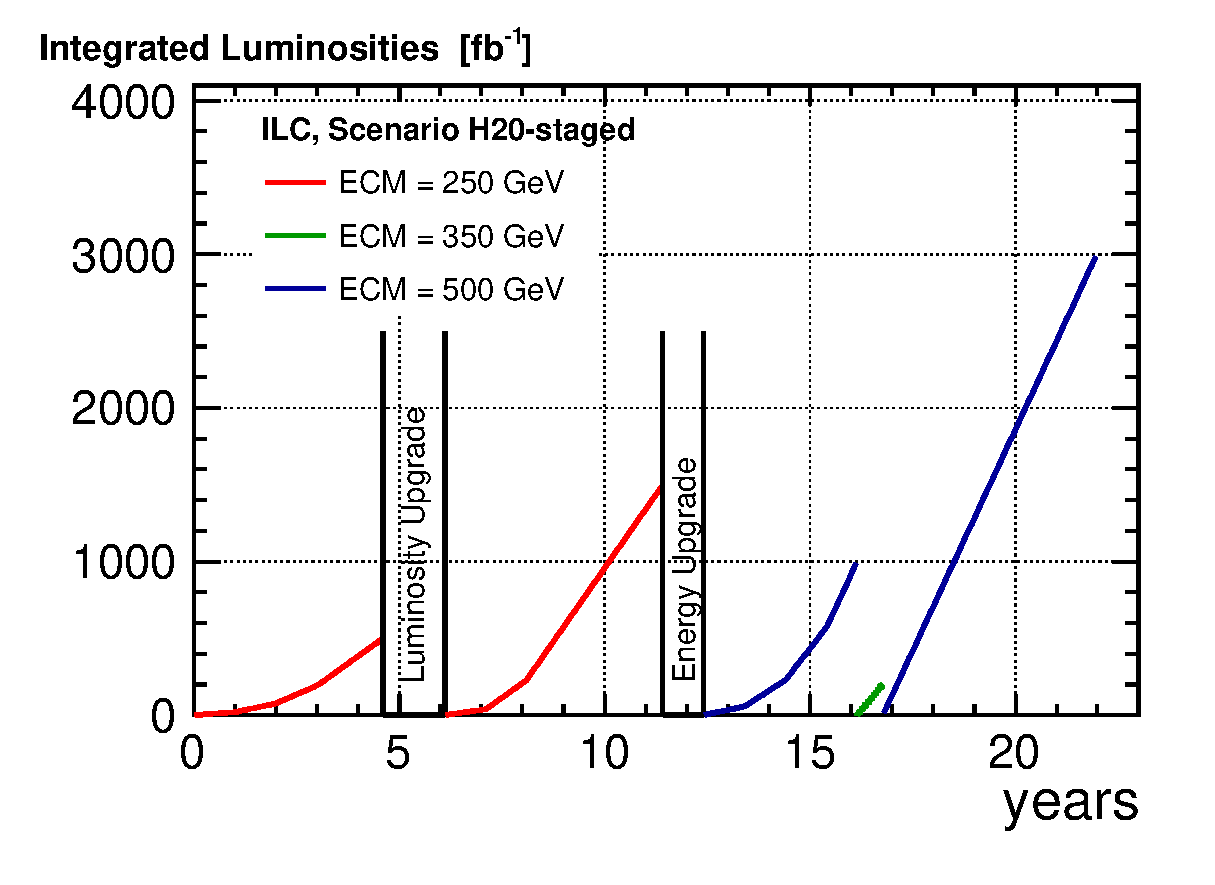
\includegraphics[width=0.75\hsize]{chapters/figures/lumi_H20-staged}
\end{center}
\caption{The nominal 22-year running program for the staged ILC, starting operation at 250\,\GeV ~\cite{Fujii:2017vwa}. The integrated luminosities are the same of for the original H20 scenario.}
\label{fig:H20staged}
\end{figure}
%%%%%%%%%%%%%%%%%%%%%%%%%%%%%%%%%%%%%%%%%%%%%%%%%%%%%%%%%%%%%%%%%%%%%%%%%%%



   
   
\section{\label{sec:physics}Physics Case (250 GeV) }

10 pages Peskin
 
% section on the physics case


The core of the physics case for the ILC is to make high-precision
 measurements of the properties of the Higgs boson.    The Higgs
 field is at the core of
 the SM.  It is responsible for the masses of all known
 elementary particles.
  It is also responsible for those aspects of the SM that are
 hardest to  understand----the
presence of spontaneous gauge symmetry breaking, the  hierarchy of quark and lepton masses, and the appearance of flavor mixing and $CP$ violation in weak 
interactions.
If we wish to learn more about these features of the fundamental laws of nature, an obvous course is to measure the Higgs boson as well as we are able.  We will argue in this section and the succeeding ones that ILC will be able to determine the mass of the Higgs boson to a part in $10^4$ and the major couplings of the Higgs boson to than 1\% accuracy.   This will qualitatively sharpen the picture of the Higgs boson that we will obtain even from the high-luminosity stage of the LHC. 

This set of measurements, and other measurements available for the first time at the ILC, will open new paths in the search for new fundamental interactions beyond the SM. 
Though the SM seems to account for all elementary particle phenomena observed up to now, it is manifestly incomplete.   It not only does not answer but actually is incapable of answering the questions posed in the previous paragraph.  It also cannot address basic facts about the universe in the large, in particular, the excess of matter over antimatter and the origin of the cosmic dark matter.  To make progress, we need observational evidence from particle physics of violations of the SM.  These will provide clues that can show the way forward.

Up to now, we have sought evidence for new interactions from direct searches for new particles at LEP, the Tevatron, and the LHC, from measurements of the $W$ and $Z$ bosons, and from searches for anomalies in flavor physics.  We are now approaching the limits of these techniques with current particle physics facilities.  The ILC will 
extend our search capabilities in precision measurements of $W$ boson couplings and fermion pair production, and will provide new opportunites for the direct discovery of new particles.  But, most of all, it will open a completely new road through the thorough, high-precision study of the Higgs boson. 


\subsection{Mysteries of the Higgs boson}

We often hear from our colleagues that the Higgs boson, as observed at the LHC, is an uninteresting particle, since it conforms so well to the expectations from the SM.   In fact, aside from our knowledge of the Higgs boson mass, the measurements make so far at the LHC tell us almost nothing about the true nature of this particle.   We now 
explain this statement, and, in the process, clarify the requirements for measurements of the Higgs boson couplings that can give insight into physics beyond the SM. 

New physics can correct the Higgs boson couplings in many ways.  However, in all cases, the size of the corrections is limited by the Decoupling Theorem, enunciated by Haber in \cite{Haber:1994mt}:    If the new particles that modify the SM have minimum mass $M$, then  the corrections to the SM predictions for the Higgs boson couplings are of size 
\beq 
              a \,     m_h^2 / M^2   \  .
\eeqn
where the coefficient $a$ is of order 1.   The exclusions of new particles through searches at the LHC suggest that $M$ is at least close to 1~TeV.   Then the effects of  new physics are limited to the few-percent level.   We will illustrate this result with explicit models in the next subsection.

The proof of the theorem is simple and illustrative.   It can be shown that the SM is actually the most general renomalizable quantum field theory with $SU(3)\times SU(2)\times U(1)$ gauge symmetry and the known particle content.   If we add new particles with masses of $M$ and above, we can assess their influence on the Higgs boson by integrating them out of the theory.  This adds to the Lagrangian a set of new terms with the SM symmetries.   The terms in the new Lagrangian  can be organized by their operator dimension 
as 
\beq 
   {\L}  =  {\L}_{SM} + {1\over M^2} \sum_i\,  c_i \O_{6i} + {1\over M^4 } \sum_j\,  d_j\O_{8j} + \cdots
\eeq{geneffL}
where $\L_{SM}$ is the SM Lagrangian with modified parameters, $\O_{6i}$  are operators of dimension 6, $\O_{8j}$ are operators of dimension 8, \etc.   The shifts in the SM parameters are not observable, since these parameters are in any case fit to experiment.  Then the leading observable corrections are of order $M^{-2}$. 

This theorem has a striking consequence.  Instead of a model with a single Higgs doublet, as we have in the SM, nature could be providing  a model with two or more Higgs fields, composite Higgs fields, even a whole Higgs sector.  All of this possible complexity is hidden from us by the Decoupling Theorem. 

The theorem has an appealing corollary, though.   Since the SM is the most general renormalizable model, once its parameters are known, its predictions for the Higgs couplings are determined precisely.   These predictions do depend on measured SM parameters such as $m_b$, $m_c$, and $\alpha_s$, but  it is argued in \cite{Lepage:2014fla} that  
lattice QCD will determine these well enough to fix the SM predictions for Higgs to part-per-mil accuracy.   Then, if we can observe corrections to the SM predictures at the 1\% level, these corrections and the evidence that they give for new physics cannot hide.

\subsection{Examples of  new physics influence on the Higgs boson}

Many models of physics beyond the SM illustrate the points made in the previous section. Here are some examples.   These examples point to  a goal of 1\% accuracy
for the measurement of Higgs boson couplings in the major decay modes.

Models with two Higgs doublets contain 5 physical Higgs particles: two  neutral $CP$-even states $h$, $H$,  a neutral $CP$-odd state $A$, and a pair of charged scalars $H^\pm$.  These states are mixed by two angles $\alpha, \beta$. The lighter
$CP$-even state $h$ is identified with the observed Higgs boson.  Its couplings to 
fermions depend on the mixing angles.   For example, in the ``Type II'' case, 
\beq
   g(hb\bar b) = - {\sin\alpha\over \cos\beta}{m_b\over v}  \quad   g(hc\bar c) =  {\cos\alpha\over \sin\beta}{m_c\over v}   \ .
\eeqn{typeIIbcshift}
However, the mixing angles are connected to the masses in such a way that when the additional bosons become heavy, their effects in \leqn{typeIIbcshift} also become small,
\beq
     - {\sin\alpha\over \cos\beta} =  1 + \O({m_Z^2\over m_A^2}) \ .
\eeqn
conforming to the Decoupling Theorem.   In Type II models, the $b$ and $\tau$ Yukawa couplngs are shifted together by about 5\% for $m_A = 500$~GeV, and by decreasing amounts when all of the additional bosons become heavier.

%%%%%%%%%%%%%%%%%%%%%%%%%%%%%%%%%%%%%%%%%%%%%%%%%%%%%%%%
\begin{figure}
\begin{center}
\includegraphics[width=0.90\hsize]{chapters/figures/WellsZhang.pdf}
\end{center}
\caption{Deviation from the SM prediction for the $hb\bar b$ 
coupling over a parameter space of grand-unified SUSY models, from \cite{Wells:2017vla}.   
Models in the upper left-hand corner are excluded by current LHC searches.  
Models above the dashed line are expected to be excluded at the  HL-LHC. 
The color-code indicates the magnitude of the coupling deviation, in \%. }
\label{fig:WellsZhang}
\end{figure}
%%%%%%%%%%%%%%%%%%%%%%%%%%%%%%%%%%%%%%%%%%%%%%%%%%%%%%%%%%%%%%


Supersymmetry (SUSY) models contain Type II  two-Higgs-double sectors, but they also contain other effects that modify the Higgs boson couplings.   Mixing between the scalar partners of $b_L$ and $b_R$ can generate a shift of the $hb\bar b$ coupling through loop diagrams.  The magnitude of this effect in 
grand-unified SUSY models is shown in 
Fig.~\ref{fig:WellsZhang}~\cite{Wells:2017vla}.   
Note that it is possible to have a large shift of the Higgs boson coupling for 
parameter values where the SUSY particles are too
heavy to be discovered at the LHC.   Thus, the search for shifts in the Higgs couplings away from the SM predictions provides a method of searching for this new physics that is indepedent of, and largely orthogonal to, the direct search for SUSY particles.   Other surveys of this effect in \cite{Cahill-Rowley:2014wba,Kanemura:2015mxa}  confirm this idea.

SUSY models typically predict very small shifts of the $hWW$ and $hZZ$ couplings, but other types of models can affect these couplings directly.   Models in which the electroweak phase transition becomes first-order and allows baryogenesis at the weak scale often involve mixing of the Higgs field with a heavy singlet field.  This gives
\beq
           g(hWW) = {2m_W^2\over v} \cos^2\phi\approx  {2m_W^2\over v} (1 -\half \phi^2) \ ,
\eeqn{scalarmixing}
where $\phi \sim  m_h/m_S$, and similarly for the $hZZ$ coupling~\cite{Hscalarmixing}   In composite models of the Higgs
 field, the Higgs field often appears as a Goldstone boson of a new strong interaction theory, giving a coupling modification by $(1- v^2/f^2)^{1/2}$, where $f$ is the Goldstone boson decay constant~\cite{HiggsasGB}.  This effect is similar to that in \leqn{scalarmixing}.

Models of Higgs compositeness, ``Little Higgs'' models, and models with extra space dimensions all contain new heavy vectorlike fermions $T$.   Typically, these fermions obtain a fraction of their mass from the Higgs mechanism (perhaps by mixing with the top quark) that is of order $m_t^2/m_T^2$.   Then they induce corrections of this order to the loop-generated Higgs couplings $g(hgg)$ and $g(h\gamma\gamma)$.  Corrections as large as 10\% can be generated in specific models~\cite{Han:2003gf}.   These same mixing and compositeness effects modify the $ht\bar t$ coupling~\cite{Agashe:2004rs}.

An interesting picture emerges.   Almost all models of new physics generate corrections to the Higgs boson couplings.   Almost always, these corrections are small, below the 10\% level, in accord with the Decoupling Theorem.  However, in precision experiments that make these coupling deviations  visible, each type of new physics affects the Higgs couplings in different ways.  In general,
\begin{itemize}
\item The $hb\bar b$ and $h\tau\tau$ couplings are sensitive to models with additional Higgs doublets.
\item The $hb\bar b$ coupling is sensitive to heavy SUSY particles with left-right mixing.
\item The $hWW$ and $hZZ$ couplings are sensitive to mixing of the Higgs field with singlet fields, and to composite structure of the Higgs boson.
\item The $hgg$ and $h\gamma\gamma$ are sensitive to models with new vectorlike fermions.
\item The $ht\bar t$ coupling is sensitive to models with composite Higgs bosons and top quarks.
\end{itemize}

In each new physics model, the  deviations from the SM predictions for the Higgs couplings form a pattern.  With precision experiments, it is possible not only to discover the existence of new physics but also to read the pattern and gain clues as to the way forward.   A worked example of such model discrimination at the level of precision expected at the ILC  is presented in
Section~7 of  \cite{Barklow:2017suo}.


\subsection{Limitations of the LHC measurements on the Higgs boson}

Today, the LHC experiments are achieving 20\% uncertainties in their measurements of Higgs boson couplings.   Over the lifetime of the LHC, including its high-luminosity stage, these experiments will acquire a factor of 30 more data.   Shouldn't this lead to Higgs coupling measurements of the required high precision?  We believe that the answer to this question is no.   We give a high-level argument here. A detailed comparison of the expected ILC capabilities with those of the high-luminosity LHC will be presented in Sec.~\ref{subsec:higgs:ilclhc}.

We find three points relevant to this comparison.  First, the measurement of Higgs boson 
decays at the LHC is extremely challenging because of the difficulty of distinguishing 
signal from background.
In the two decay modes in which the Higgs boson was discovered, $h\to \gamma\gamma$ and $h\to 4\ell$, Higgs events are apparent, because all products of the Higgs are observed and the Higgs mass can be reconstructed with high accuracy.  Unfortunately, these modes correspond to tiny branching ratios,  0.2\% and and 0.02\% of Higgs decays, respectively.  For more typical decay  modes, Higgs boson decay events have no obvious differences in appearance from SM background reactions with larger rates.   For example, $h\to WW\to e\nu \mu \nu $ events differ from $q\bar q\to WW \to  e\nu \mu \nu $ events only in subtle features of the lepton momentum distributions.  To discover the Higgs boson in one of the major channels, the LHC experiments start from samples that are 10:1 background to signal (for $h\to b\bar b$, the ratio is 20:1). They then  extract the signal by significant kinematic cuts and the use of machine-learning classifiers.  It is already a triumph that ATLAS and CMS have been able to obtain significant observations. 

Measuring  the Higgs couplings with high precision is even more of a challenge.   It is currently beyond the state of the art to determine the efficiency  with which SM background events pass the cuts of a Higgs analysis to 1\% accuracy.   These background events must be subtracted from the Higgs signal, and so this 1\% would translate to a 10\% accuracy on the Higgs $\sigma\times BR$ or a 5\% error on the coupling. To go beyond this level is truly daunting.  Nevertheless, the studies reported in the HL-LHC Yellow Book~\cite{xxx} give reasons for optimism and cite goals of 2-4\%  for Higgs coupling uncertainties.

This brings us to the secoind point.  As we have emphasized already, the modifications of the Higgs boson couplings from new  physics are expected to be small.  In the previous section, we have argued that new physics interactions are expected to affect specific
Higgs boson couplings at a level of order 5\% or smaller.  A 2\% measurement of such a coupling  
would not meet the $3\sigma$ criterion for positive evidence of new physics.

Finally, one must take into account that the HL-LHC measurements will ultimately be limited by the systematic understanding of backgrounds  An deviation in Higgs couplings observed at the LHC is then likely to be questioned (as, for example, the $t\bar t$ forward-backward asymmetry from the Tevatron was) without a clear means of confirming the result. 
One sometimes hears that the LHC can measure ratios of branching ratios with improved accuracy, but this statement is wrong for the major modes, since each mode has different backgrounds and requires its own dedicated analysis. 

 In contrast, as we will argue below, the observation of Higgs coupling deviations at the ILC at  250~GeV would be statistics-limited and can be confirmed by experiments at 500~GeV that bring in a new production reaction with an independent, data set. 


\subsection{$\ee\to Zh$}

The arguments just presented call out for a different way to measure Higgs boson couplings.   In this method, Higgs boson events should be apparent with a simple discriminator that can then be refined for high-accuracy $\sigma\times BR$.  Ideally, this method should identify Higgs boson events independently of the decay mode, allowing the measurement of the total cross section for Higgs production and the discovery of exotic and unanticipated Higgs decays.

This new method will be provided by the ILC.  It is the measurement of the reaction $\ee\to Zh$ at 250~GeV.   At an $\ee$ collider at this energy, it is true to a first approximation that any $Z$ boson observed with a lab energy of  110~GeV is recoiling against a Higgs boson.   The backgrounds to this signature (present at about 30\% of the signal level before cuts)  come from radiative $\ee\to Z\gamma$ and $\ee\to ZZ$, reactions that are well-understood and computed from electroweak theory at the 0.1\% level. 

The reaction $\ee\to Zh$ provides {\it tagged} Higgs decays.   Thus, events can be selected independently of the Higgs decay mode.  Then (1) the  total cross section for this reaction can be measured, giving a means of absolutely normalizing Higgs boson couplings; (2)  Higgs branching ratios can be measured  by counting, independently of the production cross section; and, (3)  exotic decay modes of the Higgs boson can be observed as products recoiling against the $Z$ tag.   Some event displays, from full 
simulation, are shown in Fig.~\ref{fig:HiggsEvents}. 

%%%%%%%%%%%%%%%%%%%%%%%%%%%%%%%%%%%%%%%%%%%%%%%%%%%%%%%%
\begin{figure}
\begin{center}
\includegraphics[width=0.5\hsize]{chapters/figures/htotautau.pdf}\ \ 
\includegraphics[width=0.40\hsize]{chapters/figures/htobb.pdf}
\end{center}
\caption{Event displays of $\ee\to Zh$ events  with $Z\to \mu^+\mu^-$, from full simulation: Left: $h\to \tau^+\tau^-$, ILC detector model;  Right: $h\to b\bar b$, SiD detector model.}
\label{fig:HiggsEvents}
\end{figure}
%%%%%%%%%%%%%%%%%%%%%%%%%%%%%%%%%%%%%%%%%%%%%%%%%%%%%%%%%%%%%%

\subsection{Search for exotic Higgs decays}

The fact that the reaction $\ee\to Zh$ yields {\it tagged} Higgs decays opens the 
possibility of another type of search for new physics.
The Higgs field is unique among SM fields in that it can form a dimension-2 operator 
$\Phi^\dagger \Phi$ with zero SM quantum numbers.  If there is any sector of fields that contains its own scalar field $\Sigma$, there will in general be a renormalizable coupling 
\beq
          \Delta \L   =   \eta\    (\Phi^\dagger \Phi) \, (\Sigma^\dagger \Sigma)  \ .
\eeq{Higgsportal}
The coupling constant $\eta$ is dimensionless, so the connection can be made at any (high) mass scale.   Thus it is possible for the Higgs boson to access a sector of elementary particles that have no other connection to the fields of the SM. 

If there is a new sector of particles with zero SM quantum numbers such that some of those particles have pair-production thresholds below 125 GeV, those particles should appear in Higgs boson decays.   If the particle that makes up cosmic dark matter is light enough to be produced in this way, the Higgs boson will have decays to invisible final states.   It is also possible that the new particles are unstable with respect to decay back to SM models.   A variety of scenarios are possible here, including decays to $4b$,
$4\tau$, $b\bar b$ + invisible states, and exotic particles with long lifetimes~\cite{Curtin:2013fra}.   With the data sample of the 250~GeV ILC, it is possible to search for all of these possible decay modes.   For  invisible Higgs decays, the expected 95\% CL exclusion limit on the  branching ratio is  $3\times 10^{-3}$, 
and for 
visible or partially visible modes the limits are in the range $10^{-3}$--$10^{-4}$~\cite{Liu:2016zki}. 

\subsection{Effective Field Theory framework for Higgs coupling determinations}
\label{subsec:phys_eft}

Though the goals of measuring the SM and exotic branching ratios of the Higgs boson are already very important, experiments at the ILC allow a further step.   The theory predictions described in Section~x.2 refer to absolute partial decay widths.   These are 
related to the Higgs branching ratios by 
\beq
           \Gamma(h\to A\bar A) =   \Gamma_{tot} \cdot BR(h\to A\bar A)  \  .
\eeqn
The Higgs boson total width is very small---4~MeV in the SM---and it is not expected that any proposed collider can measure this value directly  with percent-level precision.
However, as we will now show, the ILC can determine the total width of the Higgs in a 
way that is highly model-independent and allows a 1\% absolute normalization of Higgs coupling constants.

A possible method to determine the Higgs width is to multiply each $hAA$ coupling by a parameter $\kappa_A$, and then fit these prarameters using data from $\ee\to Zh$.   In this simple method, the total cross section for $\ee\to Zh$ is proportional to $\kappa_Z^2$ and so the $\kappa_A$ parameters can be absolutely normalized.   This method has been used in much of the literature on Higgs coupling determinations, including \cite{Fujii:2015jha}.  In that paper, invisible and visible but exotic decay modes were treated by including these two partial widths as two additional parameters in the fit.  Using as inputs the measureable $\sigma\times BR$s for SM Higgs decay channels and Higgs decays to invisible final states, plus the total cross section for $\ee\to Zh$,  the ILC data would give a well-defined fit to the $\kappa_A$ parameters.

There are two problems with this method.  First, it is not completely model-independent.  Modelling the effects of new physics as a general set of dimension-6 operators as in \leqn{geneffL}, we find two different Lorentz structures for the modifications of the $hZZ$ vertex,
\beq
   \Delta \L =    (1 + \eta_Z) {m_Z^2\over v}  h Z_\mu Z^\mu + \zeta_Z {1\over 2v} h
   Z_{\mu\nu} Z^{\mu\nu} \ ,
\eeq{etazeta}
and a similar pair of structures for the $hWW$ vertex.  In principle, the two coefficients  in each case should be independently determined from data.  Second, the method does not make the most effective use of the data set from $\ee$ colliders.  The total width of the Higgs boson is determined from the ratio  $\sigma(\ee\to Zh)/\Gamma(h\to ZZ^*)$.  Since the denominator is a 3\% branching ratio, this strategy sacrifices a factor 30 in 
statistics.

A much more effective method for fitting Higgs boson couplings is described in \cite{Barklow:2017suo}.   In this method, we model the effects of new physics by the most general set of dimension-6 operators that can appear in \leqn{geneffL}.  The complete set of $SU(3)\times SU(2)\times U(1)$-invariant lepton- and baryon-number conserving dimension-6 operators  includes 59 terms~\cite{Grzadkowski:2010es}.  However, for 
the analysis of $\ee$ collider data, we can restrict ourselves to electron reactions 
producing the Higgs boson and other color-singlet states. To compute deviations from the SM predictions, it suffices to work at the electroweak tree level in the effective Lagrangian coefficients. (Of course, the SM predictions themselves must be worked out to high precision.)   We can consider $CP$-even observables; the contributions of $CP$-odd operators can be bounded by independent measurements.   With these simplifications, a total of 17 operators coefficients appear in the analysis.   To determine these coefficients, we can use precision electroweak measurements and data on $\ee\to W^+W-$ in addition to data from Higgs processs.   It is shown in 
\cite{Barklow:2017suo} that this data suffices to determine independently  the 17 operator coefficients, plus 4 SM parameters (which must be refit in the new context), plus the two partial widths for invisible and exotic Higgs decays. 


%%%%%%%%%%%%%%%%%%%%%%%%%%%%%%%%%%%%%%%%%%%%%%%%%%%%%%%%
\begin{figure}
\begin{center}
\includegraphics[width=0.80\hsize]{chapters/figures/Zhdiagrams.pdf}
\end{center}
\caption{Feynman diagrams contributing to the process $\ee\to Zh$ when contributing  dimension-6 operators are included. }
\label{fig:eeZhdiagrams}
\end{figure}
%%%%%%%%%%%%%%%%%%%%%%%%%%%%%%%%%%%%%%%%%%%%%%%%%%%%%%%%%%%%%%


Beam polarization plays an important role in the analysis.   Including the effects of dimension-6 operators, the process $\ee\to Zh$  involves three Feynman diagrams, shown in Fig.~\ref{fig:eeZhdiagrams}.   Only the first diagram appears in the SM analysis; the other two are generated by dimension-6 operators.   The third diagram is required to be small by precision electroweak constraints.  The second diagram is generated by the same operators that generate the $\zeta_Z$ coefficient in \leqn{etazeta}.   Under a spin reversal $e^-_L \leftrightarrow e^-_R$, the first diagram flips sign while the second diagram keeps its sign.  Thus,  measurement of the 
polarization asymmetry  in the total cross section for $\ee\to Zh$ directly measures the $\zeta$ parameter in \leqn{etazeta}.   (In a similar way, measurement of the forward-backward asymmetry in $\ee\to Zh$ tests for the presence of a $CP$-violating dimension-6 contribution.)

After we describe the experimental methods and the expected measurement uncertainties in Section~VII, we will present the projections for uncertainties in 
Higgs couplings that follow from the use of this method.  Suffice it to say that the data set expected for the ILC at 250~GeV is expected to measure the $hb\bar b$ couplings to 1\% accuracy, the $hWW$ and $hZZ$ couplings to better than 0.7\%, and the other 
major SM Higgs couplings to accuracies close to 1\%.    These measurements should be 
statistics-limited.  Above 250~GeV, a second Higgs production reaction, $\ee\to \nu\bar\nu h$ through $W$ boson fusion becomes important.  Using the additional data on $\ee\to Zh$ and the independent measurements from the $W$ fusion reaction, we expect that the uncertainties on Higgs couplings will decrease by another factor of 2. 


\subsection{$\ee \to W^+W^-$}
\label{subsec:phys_WW}
The reaction $\ee\to W^+W^-$ contributes to the analysis just described, but it has its own independent interest.  It has been appreciated for  a long time that this reaction provides an excellent way to test for the presence of dimension-6 operators that involve the $W$ and $Z$ fields.   The Feynman diagrams contributing to the reaction are shown in Fig.~\ref{fig:WWdiagrams}.   The process involves interference between $s$-channel diagrams with $\gamma$ and $Z$ exchanges and a $t$-channel diagram with neutrino exchange.  In the SM, there are large cancellations among these diagrams, but these are not respected by the dimension-6 contributions.   Thus, the dimension-6 coefficients appear in the cross section formulae enhanced by a factor $s/m_W^2$. 

%%%%%%%%%%%%%%%%%%%%%%%%%%%%%%%%%%%%%%%%%%%%%%%%%%%%%%%
\begin{figure}
\begin{center}
\includegraphics[width=0.80\hsize]{chapters/figures/WWdiagrams.pdf}
\end{center}
\caption{Feynman diagrams contributing to the process $\ee\to W^+W^-$ when contributing  dimension-6 operators are included.}
\label{fig:eeWWdiagrams}
\end{figure}
%%%%%%%%%%%%%%%%%%%%%%%%%%%%%%%%%%%%%%%%%%%%%%%%%%%%%%%%%%%%%%

The largest part of the dimension-6 effect can be described by shifts of the form 
factors for the $WW\gamma$ and $WWZ$ vertices.  These vertices can be parametrized as \cite{Hagiwara:1986vm}
\beq
\Delta \L = 
\eeq{WWgZvertex}
where $V = A,Z$.  In the SM, $g_{1A} = e$, $g_{1Z} = e s_w/c_w$ and the other coeficients are zero at the tree level.   The result $g_{1A} = e$ is exact due to the QED Ward identity.  The dimension-6 operator corrections generate a 3-parameter shift of the other 5 coefficients. These shifts can in principle be measured both at electron and at hadron colliders.  However, measurements in $\ee$ have  definite advantages.   First, it is possible to use final states with hadronic $W$ decays to determine the complete kinematics of each event and, using this information, to separate the production of 
transverse and longitudinal $W$ bosons.   Then, using beam polarization and $W$ final-state polarization, the 3 possible shifts of the form factors can be measured separately.   Second,  the greater intrinsic accuracy of measurements in $\ee$ give excellent results at a center of mass energies of 250--500~GeV.  At hadron colliders, 
the factor $s/m_W^2$ can be much larger, and one can take advantage of this by observing the reaction at $WW$ pair masses above 1~TeV.  However, this can lead to ambiguities due to the possible influence of dimension-8 operators, whose effects grow as $(s/m_W^2)^2$~\cite{Falkowski:2016cxu}. 

In Section VII  below, after describing the experimental study of $\ee\to W^+W^-$, we will show that the ILC at 250~GeV is expected to improve the precision of $W$ form factor measurements by an order of magnitude over expected results from HL-LHC.




\subsection{$\ee\to f\bar f$}
\label{subsec:phys_ff}

Fermion pair production provides a search for new forces that couple directly to the electron.   At LEP and LHC, $\ee$ and $q\bar q$ annihilation are used as probes for new gauge bosons appearing in the $s$-channel and for signals of fermion compositeness. 

The comparison with LEP 2 is instructive.   The ILC will operate at an energy not so far above that of LEP 2  (250~GeV {\it vs.}  180--208~GeV)  but with much higher luminosity (2 ab$^{-1}$  {\it vs.} a total of 1~fb$^{-1}$ over 4 experiments).   For statistics-limited measurements, this gives a factor 
\beq
   \biggl[{  s \cdot \int \L |_{ILC}\over s \cdot \int \L|_{LEP}} \biggr]^{1/2} \approx 
                    60 
\eeqn
improvement in sensitivity to deviations from the SM, or an improvement of  7.5 in the mass scale that can be accessed.   Though the comparison depends on the particular model, this corresponds to the ability to observed new vector bosons at 5--6 TeV and 
contact interaction scales of 70~TeV, comparable to  the projected reach of the HL-LHC. 

 In addition, the information from ILC is very specific.   Measuring the cross section for $\ee\to f\bar f$ in the forward and backward directions for $e^-_L$ and $e^-_R$ beams gives four  different observables, each of which corresponds to a different dimension-6 effective  interaction.   Discovery of an anomaly points directly to a model interpretation, either with an $s$-channel resonance or with new interactions at higher energy.   This information can be put together with results of resonance searches at the LHC. 

The reaction $\ee\to b\bar b$ deserves special consideration. In models in which the Higgs boson is composite, typically either the $t_L$ or the $t_R$ must be composite also to generate a large enough $t$ quark mass.    The $b_L$ is the $SU(2)$ partner of the $t_L$ and so must have the same admixture of composite structure.    If it is the $t_R$ that is more composite, it is not required that the $b_R$ is composite, but this often happens in models.  This can generate few-percent corrections to the rates for $e^-_{L,R} e^+\to b_R\bar b_L$ at the ILC.  ~\cite{Funatsu:2017nfm,YoonPeskin}.   It is possible that this effect, rather than effects in Higgs decays, would be the first indication of a composite Higgs sector. 

     
\subsection{Search for pair-production of new particles}

Despite the wide range of direct searches for new particle pair production at the LHC, 
those searches have blind spots corresponding to physically interesting models.  The two most important of these are:
\begin{enumerate}
\item  Insensitivity to new particles with electroweak interactions only that decay to an invisible partner with a mass gap of less than 5~GeV.   Though this case seems quite special, this is exactly the set of properties predicted for the charged Higgsino of SUSY models.  Dark matter scenarios involving coannihilation can also all into this blind spot, since in those models there is an electroweak partner separated from the dark matter particle by $k_B T$ at the thermal dark matter freezeout temperature of 5-10~GeV.
\item Insensitivity to production of pairs of invisible particles observed through radiation of an initial-state gluon.   At the LHC, such ``mono-gluon'' events have as a background initial state radiation in the Drell-Yan process, and the sensitivity to such events is limited by the precision of our knowledge of the Drell-Yan cross section.
\end{enumerate}
In both cases, the ILC can detect these new physics events for particle masses almost up to half of  the collider center of mass energy.

The experimental aspects of these particle seaches are discussed in Section~VIII.  A broader review of the opportunities for new particle discovery at $\ee$ colliders can be found in \cite{Fujii:2017ekh}.

 
\section{\label{sec:detectors}Detectors }


  10 pages Behnke + White
  
The ILC accelerator is currently planed with one interaction region, quipped with two experiments. The two experiments are swapped into the Interaction Point within the so-called "Push-Pull" scheme. The experimente have been designed to allow fast move-in and move-out from the interaction region, on a timescale of a few hours to a day. In 2009 a call for letters of intent was issued to the community. Two experiments were eventually selected and invited to prepare more detailed proposals, the SiD detector and the ILD detector. Both prepared detailed and costed proposals which were scrutinised by an international advisory panel, and included in the ILC technical design report in 2012. In this section the two proposals are briefly introduced.

\subsection{SiD Detector - Introduction}
The SiD detector is a general-purpose experiment designed to perform precision measurements
at ILC. It satisfies the challenging detector requirements resulting from the full range of ILC physics processes. SiD is based on the paradigm of particle flow, an algorithm by which
the reconstruction of both charged and neutral particles is accomplished by an optimised
combination of tracking and calorimetry. The net result is a significantly more precise jet
energy measurement which results in a di-jet mass resolution good enough to distinguish
between W’s and Z’s.
The SiD detector (Fig.~\ref{fig:fig_sid})is a compact detector based on a powerful silicon
pixel vertex detector, silicon tracking, silicon-tungsten electromagnetic calorimetry and
highly segmented hadronic calorimetry. 
SiD also incorporates a high-field solenoid, iron
flux return, and a muon identification system. The use of silicon sensors in the vertex, tracking
and calorimetry enables a unique integrated tracking system ideally suited to particle
flow.

The choice of silicon detectors for tracking and vertexing ensures that SiD is robust
with respect to beam backgrounds or beam loss, provides superior charged particle momentum
resolution, and eliminates out-of-time tracks and backgrounds. The main tracking
detector and calorimeters are “live” only during a single bunch crossing, so beam-related
backgrounds and low-pT backgrounds from \gamgam processes will be reduced to the minimum
possible levels. The SiD calorimetry is optimised for excellent jet energy measurement
using the particle flow technique. The complete tracking and calorimeter systems are contained
within a superconducting solenoid, which has a 5 T field strength, enabling the overall
compact design. The coil is located within a layered iron structure that returns the magnetic flux and is instrumented to allow the identification of muons. All aspects of SiD are the result of intensive and leading-edge research aimed at achieving
performance at unprecedented levels. At the same time, the design represents a balance between cost
and physics performance. The key parameters of the SiD design are listed in  Table~\ref{sid:ConceptOverview:Table:Ovw_sidparams}.

\begin{figure}[tb]
 %\epsfysize=9.0cm
 \begin{center}
 \includegraphics[width=0.9\hsize]{chapters/figures/SiD.pdf}
\caption{The SiD detector concept.
\label{fig_sid}}
 \end{center}
 \vspace{-0.7cm}
 \end{figure}

%\thisfloatsetup{floatwidth=\SfigwFull,capposition=beside}
\begin{table}[htbp]
\renewcommand{\arraystretch}{1.25}

%fixme: ttabbox is not known ...
%\ttabbox{

\caption{\label{sid:ConceptOverview:Table:Ovw_sidparams}Key parameters of the baseline \sid design. (All dimension
are given in cm).}

{
\begin{tabular}{l l r r r}
    \toprule
    \sid Barrel& Technology& In rad& Out rad& z extent \\
    \midrule
    Vtx detector& Silicon pixels& 1.4& 6.0& $\pm \quad 6.25$ \\
    Tracker& Silicon strips& 21.7& 122.1& $\pm \quad 152.2$ \\
    ECAL& Silicon pixels-W& 126.5& 140.9& $\pm \quad 176.5$ \\
    HCAL& RPC-steel& 141.7& 249.3& $\pm \quad 301.8$ \\
    Solenoid& 5 Tesla SC & 259.1& 339.2& $\pm \quad 298.3$ \\
    Flux return& Scint-steel& 340.2 & 604.2& $\pm \quad 303.3$ \\
    \bottomrule

   \toprule
 \sid Endcap& Technology& In z& Out z& Out rad \\
    \midrule
Vtx detector& Silicon pixels& 7.3& 83.4& 16.6 \\
Tracker& Silicon strips& 77.0& 164.3& 125.5 \\
ECAL& Silicon pixel-W& 165.7& 180.0& 125.0 \\
HCAL& RPC-steel& 180.5& 302.8& 140.2 \\
Flux return& Scint/steel& 303.3& 567.3& 604.2 \\
LumiCal& Silicon-W& 155.7& 170.0& 20.0 \\
BeamCal& Semicond-W& 277.5& 300.7& 13.5 \\
    \bottomrule
\end{tabular}
}

\end{table}

\subsubsection{Silicon-based Tracking}
The tracking system (Fig.~\ref{fig:fig_vxdtrk}) is a key element of the SiD detector concept. The
particle flow algorithm requires excellent tracking with superb efficiency and
two-particle separation. The requirements for precision measurements, in
particular in the Higgs sector, place high demands on the momentum resolution at
the level of $\delta (1/\pT)  \sim 2-5 \times 10^{-5}/$GeV/$c$.

Highly efficient charged particle tracking is achieved using the pixel detector
and main tracker to recognise and measure prompt tracks, in conjunction with the ECAL, which can
identify short track stubs in its first few layers 
to catch tracks arising from secondary decays of long-lived particles. With
the choice of a 5~T solenoidal magnetic field, in part chosen to control the $\ee$-pair
background, the design allows for a compact tracker design. 

\begin{figure}[tb]
 %\epsfysize=9.0cm
 \begin{center}
 \includegraphics[width=0.9\hsize]{chapters/figures/vxdtrk.pdf}
\caption{r-z view of vertex detector and outer tracker.
\label{fig_vxdtrk}}
 \end{center}
 \vspace{-0.7cm}
 \end{figure}

\subsubsection{Vertex detector}

To unravel the underlying physics mechanisms of new observed processes, the
identification of heavy flavours will play a critical role. One of the main
tools for heavy flavour identification is the vertex detector. The physics goals
dictate an unprecedented spatial three-dimensional point resolution and a very
low material budget to minimise multiple Coulomb scattering. The running 
conditions at the ILC impose the readout speed and radiation tolerance. 
These requirements are normally in tension. High
granularity and fast readout compete with each other and tend to increase the
power dissipation. Increased power dissipation in turn leads to an increased
material budget. The challenges on the vertex detector are considerable and
significant R\&D is being carried out on both the development of the sensors and
the mechanical support.
The \sid vertex detector uses a barrel and disk layout. The barrel section
consists of five silicon pixel layers with a pixel size of
$20~\times~20~\micron^2$. The forward and backward regions each have four
silicon pixel disks. In addition, there are three silicon pixel disks at a
larger distance from the interaction point to provide uniform coverage for the
transition region between the vertex detector and the outer tracker. This
configuration provides for very good hermeticity with uniform coverage and
guarantees excellent charged-track pattern recognition capability and impact parameter resolution 
over the full solid angle. 
This enhances the capability of the integrated tracking system and, 
in conjunction with the high magnetic field, makes for a very compact
system, thereby minimising the size and costs of the calorimetry.

To provide for a very robust track-finding performance the baseline 
choice for the vertex detector has a sensor technology that provides
time-stamping of each hit with sufficient precision to assign it to
a particular bunch crossing. This significantly suppresses
backgrounds. 

%Several technologies are being developed. One of them is a CMOS-based
%monolithic pixel sensor called Chronopixel. The main goal for the design is a
%pixel size of about $10~\times~10~\micron^2$ with 99\% charged-particle
% efficiency. Prototype devices have demonstrated that the concept works; 
%what should be a fully functional chip is presently under test. More 
%challenging is the 3D vertical integrated silicon technology, for which a full 
%demonstration is also close.

Several vertex detector sensor technologies are being developed.  One of these is a 
monolithic CMOS pixel detector with time-stamping capability (Chronopixel~\cite{Sinev:2015iwr}),
being developed in collaboration with SRI International. 
The pixel size is about  $10~\times~10~\micron^2$ with 99\% designed charged-particle
 efficiency.
The time-stamping feature of the design means each hit is accompanied by a time tag with sufficient precision to assign it to a particular bunch crossing of
the ILC - thus the name Chronopixel. This reduces the occupancy to negligible levels, even in the
innermost vertex detector layer, yielding a robust vertex detector which operates at background
levels significantly in excess of those currently foreseen for the ILC. Chronopixel differs from the
similar detectors developed by other groups by its capability to record time stamps for two hits in
each pixel while using standard CMOS processing for manufacturing. 
Following a series of prototypes, the Chronopixel has been proven to be
a feasible concept for the ILC. The first set of prototype
devices was fabricated in 2008, the second prototype in 2012, and the third prototype in 2014.
The main goal of the third prototype was to test possible solutions for a high capacitance problem
discovered in prototype 2. The problem was traced to the TSMC 90 nm technology design rules,
which led to an unacceptably large value of the sensor diode capacitance. Six different layouts
for the prototype 3 sensor diode were tested in prototype 3, and tests have shown that the high capacitance
problem was solved.

With prototype 3 proving that a Chronopixel sensor can be successful with all known problems solved, optimal sensor design would be the focus of future tests.
The charge collection efficiency for different sensor diode options needs to be measured to determine
the option with the best signal-to-noise ratio. Also, sensor efficiency for charged particles with sufficient energy to penetrate the sensor thickness and ceramic package, along with a trigger telescope measurement, needs to be determined. Beyond these fundamental measurements, a prototype of a few cm$^2$ with a final readout scheme would
test the longer trace readout resistance, capacitance, and crosstalk.

A more challenging approach is the 3D vertical integrated silicon technology, for which a full 
demonstration is also close.




Minimising the support material is critical to the development of a high-performance 
vertex detector. An array of 
low-mass materials such as reticulated foams and silicon-carbide
materials are under consideration. An alternative approach that is being pursued very actively is the
embedding of thinned, active sensors in ultra low-mass media. This line of R\&D
explores thinning active silicon devices to such a thickness that the silicon
becomes flexible. The devices can then be embedded in, for example, Kapton
structures, providing extreme versatility in designing and constructing a vertex
detector.

Power delivery must be accomplished without exceeding the material budget and
over heating the detector.  The vertex detector 
design relies on power pulsing during bunch trains to minimise heating 
and uses forced air for cooling. 

\subsubsection{Main tracker}
The main tracker technology of
choice is silicon strip sensors arrayed in five nested cylinders in the central
region and four disks following a conical surface with an angle of 5 degrees
with respect to the normal to the beamline in each of the end regions. The geometry of the endcaps
minimises the material budget to enhance forward tracking. The detectors are
single-sided silicon sensors, approximately 10 $\times$ 10 cm$^2$ with a readout
pitch of 50~\micron. The endcaps utilise two sensors bonded back-to-back for
small angle stereo measurements. With an outer cylinder radius of 1.25~m
and a 5~T field, the charged track momentum resolution will be better than
$\delta (1/\pT) = 5 \times 10^{-5} $/(GeV/$c$) for high momentum tracks with coverage down to polar angles of 10 degrees.

The all-silicon tracking approach has been extensively tested using full Monte-Carlo
simulations including full beam backgrounds. Besides having an excellent momentum resolution
it provides robust pattern recognition even in the presence of backgrounds and has a
real safety margin, if the machine backgrounds will be worse than expected.

\subsubsection{Main calorimeters}

The \sid  baseline design incorporates the elements needed to
successfully implement the PFA approach. This imposes a number of
basic requirements on the calorimetry. The central calorimeter
system must be contained within the solenoid in order to reliably associate
tracks to energy deposits. The electromagnetic and hadronic sections
must have imaging capabilities that allow both efficient
track-following and correct assignment of energy clusters to tracks. These
requirements imply that the calorimeters must be finely segmented both
longitudinally and transversely. In order to ensure that no significant amount
of energy can escape detection, the calorimetry must extend down to small
angles with respect to the beampipe and must be sufficiently deep to prevent
significant energy leakage. Since the average penetration depth of a hadronic
shower grows with its energy, the calorimeter system must be designed for the
highest-energy collisions envisaged.

In order to ease detector construction the calorimeter mechanical design consists of a series of modules of
manageable size and weight. The boundaries between
modules are kept as small as possible to prevent significant non-instrumented
regions. The detectors are designed to have excellent long-term stability and reliability,
since access during the data-taking period will be extremely limited, if not
impossible.

The combined ECAL and HCAL systems consist of a
central barrel part and two endcaps, nested inside the barrel. The entire barrel system is contained
within the volume of the cylindrical superconducting solenoid. 

%The
%electromagnetic calorimeter has silicon active layers between tungsten absorber
%layers. The active layers use 5$\times$5~mm$^2$ silicon pixels, which provide excellent spatial resolution.
%The structure has 30 layers in total, the first 20 layers having a
%thinner absorber than the last ten layers. This configuration is a 
%compromise between cost, electromagnetic shower radius, sampling frequency, and
%shower containment. The total depth of the electromagnetic calorimeter is 26
%radiation lengths (\xo) and one nuclear interaction length. 

The SiD reliance on Particle Flow Algorithm-based (PFA) calorimetry to obtain a jet energy resolution of  $\sim$3\% demands a highly segmented (longitudinally and laterally) electromagnetic calorimeter. It also calls for a minimized lateral electromagnetic shower size, by minimizing the Moliere radius to efficiently separate photons, electrons and charge hadrons~\cite{calor:2018}.

The SiD design employs thirty longitudinal layers, the first twenty each with 2.50 mm tungsten alloy thickness and 1.25 mm readout gaps, and the last ten with 5.00 mm tungsten alloy.  The total depth is 26 radiation lengths, providing good containment of electromagnetic showers.

Simulations have shown the energy resolution for electrons or photons to be well described by 0.17 / $\sqrt{E}$ $\oplus$ 0.009, degrading some at higher energies due to changes in sampling fraction and a small leakage.

The baseline design employs tiled, large, commercially produced silicon sensors (currently assuming 15 cm wafers). The sensors are segmented into pixels that are individually read out over the full range of charge depositions. The complete electronics for the pixels is contained in a single chip, the KPiX ASIC~\cite{Brau:2013yb}, which is bump bonded to the wafer. The low beam-crossing duty cycle ($10^{-3}$ ) allows reducing the heat load using power pulsing, thus allowing passive thermal management within the ECal modules.

Bench tests of the KPiX bonded sensor  with a cosmic ray telescope trigger yielded 
a Landau distribution with a peak of the signal at about 4 fC is consistent with our expectation for minimum-ionizing particles (MIP) passing through the fully-depleted 320 $\mu$m thick sensors. Crosstalk between channels has been managed and the 
 noise distribution shows an RMS of 0.2 fC, well below the 4 fC MIP signal, and exceeding the ECal requirement.

The overall mechanical structure of the ECal barrel has been designed for minimal uninstrumented gaps. Input power and signals are delivered with Kapton flex cables.
The KPiX chip has an average power less than 20 mW, resulting in a
total heat load  that is managed with a cold plate and water pipes routed 
into the calorimeter.

A first SiD ECal prototype stack of nine (of thirty) layers has been constructed and was exposed to a 12.1 GeV electron beam at the SLAC End Station Test Beam Facility. 
This data collection demonstrated good measurements of multiple particle overlap and reconstruction of overlapping showers~\cite{Steinhebel:2017qze}.  Comparison of the deposited energy distribution in each of the nine layers also agrees well with simulations.
An algorithm developed to count the number of incident electrons in each event. The algorithm was used to assess the ability of the calorimeter to separate two showers as a function of the separation of the showers, achieving 100\% for separations of $>$10 mm.



The hadronic
calorimeter has a depth of 4.5 nuclear interaction lengths, consisting of
alternating steel plates and active layers. The baseline choice for the active
layers is scintillator tiles read out via silicon photomultipliers. For this approach SiD is closely following the analog hadron calorimeter developments within the CALICE collaboration. In this context, the simulated HCAL energy resolution has been shown to reproduce well the results from the CALICE AHCAL prototype module exposed to pion beams.

\subsubsection{Forward calorimeters}

Two special calorimeters are foreseen in the very forward region: LumiCal for a precise luminosity measurement, and BeamCal for the fast estimation of the collision parameters and tagging of forward-scattered beam particles. LumiCal and BeamCal are both compact cylindrical electromagnetic calorimeters centered on the outgoing beam, making use of semiconductor-tungsten technology. BeamCal is placed just in front of the final focus quadrupole and LumiCal is aligned with the electromagnetic calorimeter endcap. 

LumiCal makes use of conventional silicon diode sensor readout. It is a precision device with challenging requirements on the mechanics and position control, and must achieve a small Moliere radius to reach its precision targets. Substantial work has been done to thin the silicon sensor readout planes within the silicon-tungsten assembly. Dedicated electronics with an appropriately large dynamic range is under development.

BeamCal is exposed to a large flux of low-energy electron-positron pairs originating from beamstrahlung. These depositions, useful for a bunch-by-bunch luminosity estimate and the determination of beam parameters, require radiation hard sensors. The BeamCal has to cope with 100\% occupancies, requiring dedicated front-end electronics. A challenge for BeamCal is to identify sensors that will tolerate over one MGy of ionizing radiation per year. Sensor technologies under consideration include polycrystalline chemical vapor deposition (CVD) diamond (too expensive to be used for the full coverage), GaAs, SiC, Sapphire, and conventional silicon diode sensors. The radiation tolerance of all of these sensor technologies has been studied in a high-intensity electron beam. 

For SiD, the main activities are the study of these radiation-hard sensors, development of the first version of the so-called Bean readout chip, and the simulation of BeamCal tagging for physics studies. SiD coordinates these activities through its participation in the FCAL R\&D Collaboration.

\subsubsection{Magnet Coil}

The \sid superconducting solenoid is based on the CMS solenoid
design philosophy and construction techniques, using a slightly modified CMS
conductor as its baseline design. Superconducting strand count in the coextruded
Rutherford cable was increased from 32 to 40 to accommodate the higher 5~T
central field. 

Many iron flux return configurations have been simulated in two
dimensions so as to reduce the fringe field. An Opera 3D calculation with the Detector
Integrated Dipole (DID) coil has been completed.
Calculations of magnetic field with a 3D ANSYS program
are in progress. These will have the capability to calculate forces and stress
on the DID as well as run transient cases to check the viability of using the
DID as a quench propagator for the solenoid. Field and force calculations with
an iron endcap HCAL were studied. The field homogeneity improvement was found
to be insufficient to pursue this option. 

Conceptual DID construction and
assembly methods have been studied. The solenoid electrical power system,
including a water-cooled dump resistor and grounding, was established.
Significant work has been expended on examining different conductor stabiliser
options and conductor fabrication methods. This work is pursued as a cost- and
time-saving effort for solenoid construction.

\subsubsection{Muon System}
The flux-return yoke is instrumented with position sensitive detectors to
serve as both a muon filter and a tail catcher. The total area to be
instrumented is very significant - several thousand square meters. Technologies
that lend themselves to low-cost large-area detectors are therefore under
investigation. Particles arriving at the muon system have seen large amounts of
material in the calorimeters and encounter significant multiple scattering
inside the iron. Spatial resolution of a few centimetres is therefore
sufficient. Occupancies are low, so strip detectors are possible. The \sid
baseline design uses scintillator technology, with RPCs as an alternative. 
The scintillator technology uses extruded scintillator readout with wavelength 
shifting fibre and SiPMs, and has been successfully demonstrated. 
Simulation studies have shown that nine or more layers of sensitive detectors 
yield adequate energy measurements and good muon-detection efficiency and purity.
The flux-return yoke itself has been optimised with respect to the uniformity of the central solenoidal field, the external fringe field, and ease of the iron assembly. This was achieved by separating the yoke barrel and end sections along a 30 degree line as shown in (Fig. ).

\subsubsection{The Machine-Detector Interface}
A time-efficient implementation of the push-pull model of
operation sets specific requirements and challenges for many detector and
machine systems, in particular the interaction region (IR) magnets, the
cryogenics, the alignment system, the beamline shielding, the detector design
and the overall integration. The minimal functional requirements and interface
specifications for the push-pull IR have been successfully developed and
published~\cite{Platform_Agreement,IR_Layout}, to which all further IR design
work on both the detectors and machine sides are constrained.

\subsection{The ILD Detector}
The ILD detector is a proposed detector for the international linear collider, ILC. It has been developed by a proto-collaboration with the goal to develop and eventually propose a fully integrated detector for the ILC. 

The ILD detector concept has been designed as a multi-purpose detector. It should deliver excellent physics performance for collision energies between 90~Gev and 1~TeV, the largest possible energy reach of the ILC. The ILD detector has been optimized to perform excellently at the initial ILC energy of 250 GeV (for more details see \cite{ild:bib:ILDloi}, \cite{ild:bib:ILDDBD}). An artists view of the ILD detector is shown in Fig.~\ref{fig:ild_3d}. 
\begin{figure}
    \centering
    \includegraphics[width=0.35\textwidth]{../figures/ILD.pdf}
    \caption{3D-picture of the ILD detector.}
    \label{fig:ild_3d}
\end{figure}

The science which will be done at the ILC requires a true multi-purpose detector. A central element of the design has been the capability of the detector to reconstruct precisely complex hadronic final states as well as more events with leptons or missing energy in the final state. Thus traditional precision detector elements as vertex detectors are combined in an overall design philosophy called particle flow, which has been developed for optimal hadronic event reconstruction.

\subsubsection{Vertexing and Tracking}
\label{subsubsec:ILDtracker}
The high precision vertex detector positioned very closely to the interaction point is followed by a hybrid tracking layout, realised as a combination of silicon tracking with a time projection chamber, and a calorimeter system. The complete system is located inside a large solenoid providing a magnetic field of 3.5-4 T. On the outside of the coil, the iron return yoke is instrumented as a muon system and as a tail catcher calorimeter. 

The vertex detector is realised as a multi-layer pixel-vertex detector (VTX), with three super-layers each comprising two layers. The detector has a pure barrel geometry. To minimise the occupancy from background hits,
the first super-layer is only half as long as the outer two. Whilst the underlying detector technology has not yet been decided, 
the VTX is optimised for point resolution and minimum material thickness. 
	
A system of silicon strip and pixel detectors surrounds the VTX detector. In the barrel, two layers of silicon strip detectors (SIT) are arranged to bridge the gap between the VTX and the TPC. In the forward region, a system of two silicon-pixel disks and five silicon-strip disks (FTD) provides low angle tracking coverage.

A distinct feature of ILD is a large volume time projection chamber (TPC) with up to 224 points per track. The TPC is optimised for 3-dimensional point resolution and minimum material in the field cage and in the end-plate. It also allows d$E$/d$x$ based particle identification. At the ILC a TPC has a number of specific strength, which make this type of detector attractive. A time projection chamber offers true three-dimensional points, and offers many of those along a charged particle trajectory. The intrinsic disadvantage of a TPC, its slow readout speed, does not really harm the performance at the ILC, since the time between bunches is relatively long, with around 300~ns. On the other hand the large number of points offer superb pattern recognition capabilities, and allows the detailed reconstruction of kinks or decays in flight within its volume. This can be achieved at a very low material budget, rather uniformly distributed over the sensitive volume. The excellent performance of the system is particularly striking at low momenta, at a few GeV and below, where the combination of three dimensional reconstruction and low material allows the efficient and precise reconstruction of tracks. 

Outside the TPC a system of Si-strip detectors in between the TPC and the ECAL (SET), provide additional high precision space points which improve the tracking performance and provide additional
    redundancy in the regions between the main tracking volume and the calorimeters. 
\subsubsection{Calorimetry}
A highly segmented electromagnetic calorimeter (ECAL) provides up to 30 samples in depth and small transverse cell size, split into a barrel and an end cap system. For the absorber Tungsten has been chosen, for the sensitive area silicon diodes or scintillator strips are considered.
%\thisfloatsetup{floatwidth=\SfigwFull,capposition=beside}
\begin{figure}[t!]
\begin{tabular}{cc}
\includegraphics[width=0.52\hsize,viewport={0 -10 600 500},clip]{chapters/figures/material-budget-new.pdf} &
\includegraphics[width=0.5\hsize]{chapters/figures/intlen_ILD_o1_v05.pdf}
\end{tabular}
\caption[Material in the ILD detector]{Left: Average total radiation length of the material
  in the tracking detectors as a function of polar angle. Right: Total interaction length in the detector, up to the end of the calorimeter system, and including the coil of the detector.}
%\end{figure}
\label{fig:intro:material}
%\begin{tabular}{cc}

\end{figure}

This is followed by a segmented hadronic calorimeter (HCAL) with up to 48 longitudinal samples and small transverse cell size. Two 
options are considered, both based on a Steel-absorber structure. One option uses scintillator tiles of $3 \times 3$\,cm$^2$, 
which are read out with an analogue system. The second uses a gas-based readout which allows a $1 \times 1$\,cm$^2$ 
cell geometry with a semi-digital readout of each cell. 

At very forward angles, below the coverage provided by the ECAL and the HCAL, a system of high precision and radiation hard calorimetric detectors (LumiCAL, BeamCAL, LHCAL) is foreseen. These
extend the calorimetric coverage to almost $4\pi$, measure the luminosity, and  monitor the quality of the colliding beams.

\subsubsection{Coil and Yoke}
A large volume superconducting coil surrounds the calorimeters, creating an axial $B$-field of nominally 3.5-4\,Tesla.

An iron  yoke, instrumented with scintillator strips or resistive plate chambers (RPCs), returns the magnetic flux of the solenoid, and, at the same time, serves as a muon filter, muon detector and tail catcher calorimeter.

%\thisfloatsetup{floatwidth=\SfigwFull,capposition=beside}
\begin{figure}[b!]
\begin{tabular}{cc}

\includegraphics[width=0.5\hsize]{chapters/figures/deltaInvP_all_fits.png} &
\includegraphics[width=0.5\hsize]{chapters/figures/evalZ-lcfiweights_qq91new_v02-test.pdf}
\end{tabular}
\caption{\label{ild:fig:intro:tracking}(left) Momentum resolution for the ILD detector concept, as a function of the transverse momentum of the particle. (right) Flavour tagging efficiency versus purity for bottom events in sample of Z decays at 91\,GeV, and for charm events with only bottom background. )}
\end{figure}



\begin{figure}[t!]

\includegraphics[width=0.8\hsize]{chapters/figures/ild01_o1_pflow.png}

\caption{\label{ild:fig:intro:pflow}Fractional jet energy resolution
    plotted against $|\cos\theta|$ where theta is the polar angle of the thrust axis of the event. }
\end{figure}

%The main parameters of the ILD detector are summarised in Table~\ref{ild:tab:barrelpara} and table~\ref{ild:tab:endcappara}.
%\begin{sidewaystable}[thb]

\subsubsection{ILD Performance}
The performance of the ILD concept has been extensively studied using a detailed GEANT4 based simulation model and sophisticated reconstruction tools. Backgrounds have been taken into account to the best of current knowledge. 

the key technologies proposed for the ILD detector have been developed in close cooperation with R\&D collaborations and have been extensively tested. The performance numbers of key systems are based on results from prototypes, whereever possible, and extraploated to the full detector performance. This strong check against experimental results ensures that the performance numbers are reliable and are considered a realistic estimate of the ultimate detector performance. 


A key characteristics of the detector is the amount of material in the detector. Particle flow requires a thin tracker, to minimise interactions before the calorimeters, and thick calorimeters, to fully absorb the showers. Figure~\ref{ild:fig:intro:material}~(left) shows the material in the detector in radiation lengths, until the entry of the calorimeter. The right plot shows the total interaction length including the calorimeter system. 

The performance of the tracking system can be summarised by its combined momentum resolution, shown in Figure~\ref{ild:fig:intro:tracking}~(left). A resolution of $\sigma_{1/p_T} = 2 \times 10^{-5}$\,GeV$^{-1}$ has been achieved for high momenta. For many physics studies the tagging of long lived particles is of key importance. Several layers of pixel detectors close to the IP allow the reconstruction of displaced vertices, as shown in Figure~\ref{ild:fig:intro:tracking}~(right).

Calorimeter system and tracking system together enter into the particle flow performance. The performance of the ILD detector for different energies and as a function of the polar angle is shown in Figure~\ref{ild:fig:intro:pflow}. 

The few plots shown in this section illustrate the anticipated performance of the detector and illustrate the potential for precision measurements with the ILD detector. 


\section{\label{sec:software}Software and Computing}

   10 pages Gaede + Miyamoto
   
   %
% some useful macros
%
\newcommand{\fix}[1]{\textcolor{red}{\texttt{#1}}} % command for comments 
%\newcommand{\fix}[1]{} % remove all comments

\newcommand{\CPP}{C\nolinebreak\hspace{-.05em}\raisebox{.4ex}{\tiny\bf +}\nolinebreak\hspace{-.10em}\raisebox{.4ex}{\tiny\bf +}}


%Description of ILC software and computing requirements] }

\fix{ PLEASE DO NOT EDIT THIS PART IN OVERLEAF! This is work in progress!}

%Description of ILC software and computing requirements] }


\subsection{Software}

More than 15 years ago the linear collider community has started to develop common software
tools to facilitate the development and optimization of detector concepts based on realistic
simulations of physics interactions. These software tools eventually led to the creation of
a common software ecosystem called \emph{iLCSoft}~\cite{bib:ilcsoft}.
The \emph{iLCSoft} tools are used by both ILC detector concepts as well as by CLIC
and partly by CEPC and FCC.

From the start, a strong emphasis has been placed on developing flexible and generic tools
that can easily be applied to other experiments or new detector concepts. 
This approach of developing common tools wherever possible has helped considerably in
leveraging the limited manpower and putting the focus on algorithm development that
is crucial for the physics performance. 

In the next sections we will introduce the most relevant tools and algorithms and
describe their design and performance, thereby following the natural flow of data processing
from generated 4-vectors to high level physics objects.


\subsubsection{Core Software Tools}

The foundation for the development of common software was laid with LCIO~\cite{Gaede:2003ip}, the
event data model (EDM) and persistency tool for linear collider studies. At the core of LCIO is a hierarchical
EDM for any particle physics experiment, as shown in Fig.\ref{fig:lcio_edm}.
%%%%%%%%%%%%%%%%
\begin{figure}
\begin{center}
\includegraphics[width=0.60\hsize]{chapters/figures/lcio_edm_schema.png}
\end{center}
\caption{Schematic view of the hierarchical EDM in LCIO.}
\label{fig:lcio_edm}
\end{figure}
%%%%%%%%%%%%%%%%%
It provides data classes for all phases of the event processing, starting from Monte Carlo truth information,
over raw data and digitization to the final reconstruction and analysis. Objects at higher levels of the processing
point back to the lower level constituting objects. As a specific design decision, there are no pointers back to the
Monte Carlo truth but these can be added if needed using dedicated generic LCRelation objects.
These relation objects can be used to create many-to-many relations between arbitrary types in the EDM.
A special class LCGenericObject holds user defined data in named vectors of types int, float and double.
This feature is used in many test beams for conditions data and raw data from the DAQ.
LCIO provides APIs in \CPP, Java and Fortran, where today \CPP\ is used almost exclusively.


The \CPP\ application framework Marlin~\cite{Gaede:2006pj} provides an easy to use environment for developing software
modules on all levels of processing and uses LCIO as its transient data format, i.e. all data that is read in or created
by a software module (called \emph{Processor}) are stored in the \emph{LCEvent} class from LCIO. Marlin processors
are self-documenting and controlled via xml-steering files. As processors have well defined input and output data, Marlin
provides a \emph{"Plug-And-Play"} environment, where any specific algorithm can easily be exchanged with another
equivalent implementation for direct comparisons and benchmarking.


The generic detector description toolkit DD4hep~\cite{Frank:2014zya,Frank:2015ivo} provides a powerful tool for describing
the detector geometries, materials and readout properties. DD4hep follows a modular component based approach and provides
interfaces to full simulations with Geant4~\cite{Agostinelli:2002hh} via DDG4, to reconstruction programs via DDRec and to
conditions data and alignment with DDCond and DDAlign respectively, see Fig.\ref{fig:dd4hep}.
%%%%%%%%%%%%%%%%
\begin{figure}
\begin{center}
\includegraphics[width=0.90\hsize]{chapters/figures/dd4hep_simple_schema.png}
\end{center}
\caption{Schematic view of DD4hep with its main components and interfaces.}
\label{fig:dd4hep}
\end{figure}
%%%%%%%%%%%%%%%%%
DD4hep is an excellent example for the development of generic software tools for the wider HEP community and was one of the
first incubator projects adopted by the Hep Software Foundation. While it was developed to address the needs of the linear
collider community, it is now used by several other projects and is under evaluation by LHC experiments.



\subsubsection{Event Generators}

Both detector concepts have created large, realistic Monte Carlo samples with the full Standard Model physics as well as various
BSM scenarios that have been used for the physics analyses presented in the following sections.
In a first step, large generator samples with $e^+e^-$-events are created with the Whizard~\cite{Kilian:2007gr} event generator.
Whizard uses tree-level matrix elements and loop corrections to generate events with the final state partons and leptons
based on a realistic beam energy spectrum, the so called \emph{hard sub-process}. The hadronization into the visible final state
is performed with Pythia~\cite{Sjostrand:2006za} tuned to describe the LEP data.

The input spectrum is created with Guinea-Pig~\cite{Schulte:1998au}, a dedicated simulation program for computing
beam-beam interactions at linear colliders. The two dominating effects of the strong beam-beam interactions are the 
beamstrahlung leading to the available luminosity spectrum (see Fig~\ref{fig:lumi_spectrum}) and the creation of
incoherent $e^+e^-$-pairs that are the source of the dominating background at the ILC. These electrons and positrons
are predominantly created in a forward cone as shown in Fig~\ref{fig:pair_bg}. It is this cone that restricts the minimal
allowed radius of the innermost layer of the vertex detector.

%%%%%%%%%%%%%%%%
\begin{figure}
\begin{center}
\includegraphics[width=0.80\hsize]{chapters/figures/lumi_spectrum_placeholder.png}
\end{center}
\caption{Luminosity spectrum for 250 GeV.\fix{need nice plot w/ correct spectrum}}
\label{fig:lumi_spectrum}
\end{figure}
%%%%%%%%%%%%%%%%%

%%%%%%%%%%%%%%%%
\begin{figure}
\begin{center}
\includegraphics[width=0.90\hsize]{chapters/figures/pair_bg_cone_SiD.png}
\end{center}
\caption{Cone of background from incoherent $e^+e^-$-pairs, generated with Guinea-Pig and simulated in the 5 T B-field of the SiD
  detector (from~\cite{Schutz:2017ihd}).}
\label{fig:pair_bg}
\end{figure}
%%%%%%%%%%%%%%%%%

Another source of background at the ILC are $\gamma \gamma \rightarrow hadrons$ events, due to bremsstrahlung and beamstrahlung photons.
These type of events are generated for $\gamma \gamma$ cms-energies from $300~\rm{MeV~to} ~2~\rm{GeV}.$ with a dedicated generator based
on ~\cite{Chen:1993dba}, for higher energies Pythia is used.


\subsubsection{Simulation}

Both detector concepts have adopted DD4hep for describing their detector simulation models and use \emph{ddsim}, a python application that
is based on the DDG4 component, providing a gateway to full simulations with Geant4.
In DD4hep the detector geometry is implemented in dedicated \CPP modules for every subdetector and the actual parameters with dimensions
and materials are provided via compact xml-files. A large palette of predefined sub-detector drivers exists in DD4hep, allowing for an
easy implementation of a new detector concept by providing suitable compact files.
A dedicated software package lcgeo~\cite{bib:lcgeo}, which is shared by SiD, ILD and CLICdp, contains all subdetector drivers for the
detector concepts under study by these groups, together with the corresponding compact parameter files.

%%%%%%%%%%%%%%%%
\begin{figure}
\begin{center}
\includegraphics[width=0.80\hsize]{chapters/figures/SiD_tracker_simmodel.png}
\end{center}
\caption{Cut-away view of the tracking system as implemented in the \emph{SIDLOI3} simulation model (from~\cite{Behnke:2013lya}).}
\label{fig:sid_trk}
\end{figure}
%%%%%%%%%%%%%%%%%
Both detector concept groups have invested considerable effort into making their full-simulation models as realistic as possible, by
\begin{itemize}
\item following the exact dimensions and layout of detector elements from engineering models
\item implementing correct material properties
\item implementing precise descriptions of the actual detector technology
\item adding realistic amounts of dead material from supports and services, such as cables and cooling pipes
\item introducing realistic gaps and imperfections into the subdetectors
\end{itemize}
Care has been taken to include realistic material estimates in particular in the tracking region where
the material budget has a direct impact on the detector performance.
Figure~\ref{fig:sid_trk} shows the tracking detector as implemented for the SiD simulation model.
%%%%%%%%%%%%%%%%
\begin{figure}
\begin{center}
\includegraphics[width=0.80\hsize]{chapters/figures/SiD_material_budget_tracker.png}
\end{center}
\caption{Resulting radiation lengths of the tracking detectors in the \emph{SIDLOI3} simulation model (from~\cite{Behnke:2013lya}).}
\label{fig:sid_mat_budget}
\end{figure}
%%%%%%%%%%%%%%%%%
%%%%%%%%%%%%%%%%
\begin{figure}
\begin{center}
\includegraphics[width=0.80\hsize]{chapters/figures/ILD_material_budget_tracker.pdf}
\end{center}
\caption{Resulting radiation lengths of the tracking detectors in the \emph{ILD\_o1\_v05} simulation model (from~\cite{Behnke:2013lya}).}
\label{fig:ILD_mat_budget}
\end{figure}
%%%%%%%%%%%%%%%%%
The average material budget in the tracking volume of the simulation models is shown in Figures~\ref{fig:sid_mat_budget}
and~\ref{fig:ILD_mat_budget} for SiD and ILD respectively.

Before the two concepts had decided to move to the common geometry description and simulation with DD4hep, they had
implemented their detailed simulation models in Mokka~\cite{MoradeFreitas:2002kj} and slic~\cite{bib:slic}. These models
have been ported into DD4hep preserving all features and dimensions, thus resulting in equivalent simulation results.
Most of the physics analyses in the next sections are based on simulations using these older programs.

The high level of detail in the simulation models as decried above is a key prerequisite for the
realistic understanding of the expected detector performance and the physics reach of the ILC for both detector concepts.


\subsubsection{Digitzation}

The output of the detailed full simulations with Geant4 from ddsim are \emph{SimTrackerHit} and \emph{SimCalorimeterHit} objects,
that store the deposited energy in the sensitive detector elements, such as silicon wafers and calorimeter cells, together with
the position and pointers to the \emph{MCParticle} that created the energy deposition. In the digitization step, carried out in dedicated
Marlin processors, these hits are converted into \emph{TrackerHit} and \emph{CalorimeterHit} objects,
taking into account all relevant effects from the detector and the readout electronics.

The \emph{SimTrackerHits} contain the exact energy-weighted position of the individual energy depositions in a given sensitive
detector element. For silicon strip-and pixel detectors as well as the ILD-TPC, these positions are smeared according to
resolutions that have been established from test beam campaigns for the different sensor technologies, thereby including effects
from charge sharing, clustering and position reconstruction. Table~\ref{tab:ild_trk_res} shows the point resolution parameters used for ILD.



%-----------------------------------------------------------------------
\begin{table}[htb]
\centering\small
\begin{tabular}{llcl}
\hline
 Subdetector &  \multicolumn{3}{c}{ Point Resolution }  \\
\hline
        VTX    &  $ \sigma_{r\phi,z}  $ & $=$ & $ 2.8 \mu\mathrm{m}$   (layer 1)   \\
               &  $ \sigma_{r\phi,z}  $ & $=$ & $ 6.0 \mu\mathrm{m}$   (layer 2)   \\
               &  $ \sigma_{r\phi,z}  $ & $=$ & $ 4.0 \mu\mathrm{m}$   (layers 3-6)   \\


        SIT    &  $ \sigma_{\alpha_{z}}   $ & $=$ & $ 7.0 \mu\mathrm{m}$    \\
               &  $  \alpha_{z}         $ & $=$ & $ \pm 7.0^\circ $ (angle with z-axis)        \\

        SET    &  $ \sigma_{\alpha_{z}}   $ & $=$ & $ 7.0 \mu\mathrm{m}$    \\
               &  $  \alpha_{z}         $ & $=$ & $ \pm 7.0^\circ $ (angle with z-axis)        \\

       FTD     &  $\sigma_{r}$      & $=$ & $ 3.0 \mu\mathrm{m}$    \\
  \emph{Pixel} &  $ \sigma_{r_\perp}$  & $=$ & $ 3.0 \mu\mathrm{m}$    \\

     FTD       &  $ \sigma_{\alpha_r}   $ & $=$ & $ 7.0 \mu\mathrm{m}$    \\
  \emph{Strip} &  $ \alpha_{r}         $ & $=$ & $ \pm 5.0^\circ $ (angle with radial direction)        \\

       TPC    &  $ \sigma^2_{r\phi} $ & $=$ & $ (50^2+900^2\sin^2\phi + \left( (25^2/22)\times (4T/B)^2\sin\theta\right)$ \\
              &                      &     &   $(z/\mathrm{cm}) )\,\mu\mathrm{m}^2$  \\
               &  $ \sigma^2_{z}    $ & $=$ & $ (400^2+80^2\times (z/\mathrm{cm})) \,\mu\mathrm{m}^2 $ \\
               &   \multicolumn{3}{c}{ where $\phi$ and $\theta$ are the azimuthal and} \\
               &   \multicolumn{3}{c}{ polar angle of the track direction } \\
\hline
\end{tabular}
\caption[Simulated ILD tracking point resolutions.]{Effective point resolution as used in the digitization of the ILD tracking detectors.
        \label{tab:ild_trk_res} }
\end{table}
%-----------------------------------------------------------------------

In the TPC hit digitization, simulated hits that are closer than the established double-hit resolution of 2~mm in $r\phi$ and 5~mm
in $z$ are merged into one. For the silicon detectors this treatment is not necessary, due to the expected low occupancies.

The \emph{SimCalorimeterHits} contain the total energy deposited in each calorimeter cell, together with the individual depositions
from the individual Monte Carlo steps. For scintillating calorimeters Birk's Law, resulting in different light yields for different
particles, is already applied during the simulation. Dedicated digitizers take into account effects of non-uniformity of the light yield
for scintillators as well as cross-talk between neighboring channels. The latter is important in particular for the simulation of
(semi)-digital calorimeters using RPCs and is possible due to the availability of the individual simulation steps, containing
the exact position of the energy deposition.

During the calorimeter digitization a two step calibration is applied for every calorimeter type and sampling structure. In a first step
the hits are calibrated to a MIP signal and in a second step, the total energy is calibrated to an absolute value of the
cell energy in $GeV$. This calibration is an iterative procedure, based on the application of the full
\emph{particle flow algorithm }(see next subsection) to single particle events with photons and $K^0$s and thereby
repeatedly adjusting the calibration constants.


  
\subsubsection{Reconstruction}

Tracking: \\

The first step of the event reconstruction consists of identifying the trajectories of charged particles based on the positions of their
energy depositions in the detector (\emph{SimTrackerHits}), typically referred to as \emph{pattern recognition}. In a second step the
kinematic parameters of these trajectories are fitted based on the known equations of motion in a magnetic field and the errors of the
hit positions. Often both steps are carried out together, e.g. by using a Kalman-Filter and simply referred to as \emph{Tracking}.

The tracking packages in iLCSoft is called MarlinTrk and provides a generic tracking-API \emph{IMarlinTrk} and underlying fitting code,
using the Kalman-Filter package \emph{KalTest}~\cite{Li:2013cxa}.
The \emph{IMarlinTrk} interface provides code to iteratively add hits to a track segment,
thereby updating the track parameters, extrapolation of the current track state to the next measurement surface or any given point
in space. It uses LCIO as data model for the Track and TrackState with a \emph{perigee} track parameterization with
track curvature $\omega$, impact parameters $d_0$ and $z_0$ and direction parameters $\phi_0$ and $\rm{tan}(\lambda)$.
A pallete of different pattern recognition algorithms are programmed against \emph{IMarlinTrk} as shown in Fig~\ref{fig:imarlintrk}.
%%%%%%%%%%%%%%%%
\begin{figure}
\begin{center}
\includegraphics[width=0.80\hsize]{chapters/figures/IMarlinTrk_ddkaltest_new.png}
\end{center}
\caption{Schematic view of the MarlinTrk tracking tools available in iLCSoft. They are based on the LCIO event data model and the
DDRec geometry description.}
\label{fig:imarlintrk}
\end{figure}
%%%%%%%%%%%%%%%%%
ILD uses the following different algorithms in the different parts of the tracking region
(for more details see~\cite{Gaede:2014aza}):

\begin{itemize}
\item SiliconTracking\\
  Algorithm used in the innermost Si-tracking detector VXD and SIT, based an a brute-force triplet seeding followed by
  a road search using the extrapolation to the next layer provided in MarlinTrk.
\item ForwardTracking\\
  Stand alone pattern recognition in the FTD forward tracker using a Cellular-Automaton to find, a possibly large, set of
  track candidates that are reduced to a unique and consistent set through the use of a Hopfield Network.
\item Clupatra\\
  Pattern recognition algorithm for the TPC, based on a topological clustering in the outer TPC pad row layers for seeding,
  followed by a Kalman-Filter based road search inwards.
\item FullLDCTracking\\
  A collection of algorithms for merging track segments from the previous algorithms and assignments of leftover hits followed
  by a final re-fit using a Kalman-Filter.
\end{itemize}

SiD had originally developed their stand alone tracking software in the Java framework \emph{LCSim}~\cite{bib:LCSim}
using a triplet based seeding followed by a road search and a final track fit. More recently SiD has adopted the \emph{ConformalTracking}
algorithm originally developed for CLICdp. It uses a conformal mapping transforming circles going through the origin (IP)
into straight lines which are then identified using a Cellular-Automaton.


\fix{add a short paragraph on DDRec and tracking surfaces here ...}

The resulting tracking efficiencies for the ILD detector are shown as a function of the momentum and
$\rm{cos}(\theta)$ in Fig~\ref{fig:ild_trkeff}.

%%%%%%%%%%%%%%%%
\begin{figure}
  \begin{tabular}[c]{c}
    \includegraphics[width=0.95\hsize]{chapters/figures/trkEff_Momentum_ttbar_ILD_ls5_v02_publish2.png} \\
    \includegraphics[width=0.95\hsize]{chapters/figures/trkEff_theta_ttbar_ILD_ls5_v02_publish1.png}
\end{tabular}
  \caption{Tracking efficiency for the ILD detector as a function of momentum (upper) and $\rm{cos}(\theta)$ (lower).
    Blue: the standard ILD detector, Red: an alternative smaller version of ILD. \fix{make nicer plots}
of ILD.}
\label{fig:ild_trkeff}
\end{figure}
%%%%%%%%%%%%%%%%%

The normalised transverse momentum resolution $\sigma(1/p_T)$ for single-muon events the SiD detector model is shown in
Fig~\ref{fig:sid_mom_res} together with fits using the parameterisation:

\begin{equation}
  \frac{\sigma(p_T)}{p^2_T} = a~\oplus~\frac{b}{p~\rm{sin}\theta}     \label{eq:trk_res_param}
\end{equation}

%%%%%%%%%%%%%%%%
\begin{figure}
\begin{center}
\includegraphics[width=0.95\hsize]{chapters/figures/SiD_momentum_resolution.png}
\end{center}
\caption{Normalised transverse momentum resolution for single-muon events as function of momentum
  in the \emph{SIDLOI3} simulation model (from~\cite{Behnke:2013lya}). The dashed lines are fits to the data points according
  to eq.~\ref{eq:trk_res_param}.}
\label{fig:sid_mom_res}
\end{figure}
%%%%%%%%%%%%%%%%%

Comparable results are obtained for ILD and both detector concepts achieve their design goals for the momentum resolution of
$\sigma(p_T)/P^2_T  < 2 \times 10^{-5} \rm{GeV}^{-1}$ for high momentum central tracks.

%%%%%%%%%%%%%%%%
\begin{figure}
\begin{center}
\includegraphics[width=0.85\hsize]{chapters/figures/SiD_D0_resolution.png}
\end{center}
\caption{Impact parameter resolution $\sigma(d_0)$ for single-muon events as function of polar angle
  in the \emph{SIDLOI3} simulation model (from~\cite{Behnke:2013lya}).} 
\label{fig:sid_d0_res}
\end{figure}
%%%%%%%%%%%%%%%%%

The impact paramter resolution as a function of polar angle for single-muon events in SiD is shown in Fig~\ref{fig:sid_d0_res} for
different particle momenta. A resolution of a few $\mu\rm{m}$ is achieved for high mometum tracks over a large range of the polar
angle down to $\sim 20^{o}$.


The tracking software is completed with a dedicated processors for the identification and reconstruction of kinks and $V_0$s.
Tracks with kinks can arise from bremsstrahlung, typically for electrons, or a large angle deflection due to multiple scattering.
$V_0$s are almost exclusively decays of $K^0_s$ and $\Lambda^0$ as well as gamma conversions.

%----------------------------------------------
~~~\\
Particle Flow: \\

The \emph{particle flow algorithm} (PFA) aims at reconstructing every individual particle created in the event in order
to take the best available measurement for the given particle type, i.e.:
\begin{itemize}
\item charged particles\\
  using the momentum measured in the tracking detectors with the excellent resolution described  above
\item photons\\
  measured in the Ecal with an energy resolution of $\sigma(E)/E \sim  11\% / \sqrt{(E/\rm{GeV})}$ \fix{is this the correct number?}
\item neutral hadrons\\
  measured predominantly in the Hcal\footnote{hadronic showers often start in the Ecal and might extend into the Muon system -
    this is taken into account in PandorPFA} with an energy resolution of $\sigma(E)/E \sim  50\% / \sqrt{(E/\rm{GeV})}$ \fix{is this the correct number?} 
\end{itemize}

The best jet energy measurement in hadronic events would be achieved if the above algorithm would work perfectly. However in reality
there is always confusion in the assignment of individual \emph{CalorimeterHits} to Clusters and showers as well as in the assignment
of tracks to clusters. This effect is demonstrated in Fig~\ref{fig:pandorapfa_perfect} for PandoraPFA~\cite{Marshall:2015rfa}, the
implementation of PFA available in iLCSoft that is used by both detector concepts.

%%%%%%%%%%%%%%%%
\begin{figure}
\begin{center}
\includegraphics[width=0.85\hsize]{chapters/figures/pandorapfa_perfect.png}
\end{center}
\caption{Jet energy resolution for $Z'$ events as a function of the jet energy in a realistic detector for PandoraPFA.
  Also shown are the effect of \emph{confusion} and the result assuming \emph{perfect PFA} (from~\cite{Marshall:2015rfa}).} 
\label{fig:pandorapfa_perfect}
\end{figure}
%%%%%%%%%%%%%%%%%

The input to PandoraPFA are collections of Tracks, Kinks, $V0$s and collections of all digitized \emph{CalorimeterHits} together with
some geometrical information retrieved from DDRec.
Following~\cite{Marshall:2015rfa} the main steps of the algorithm are:

\begin{itemize}
\item \emph{CalorimeterHits} are clustered using a simple cone-based algorithm, seeded either from isolated hits in the first calorimeter
  layers or by the projection of Tracks to the front face of the Ecal.

\item the clustering algorithm is configured to prefer splitting of clusters rather than risking to falsly merge particles into single
  clusters.

\item Clusters are associated to Tracks based on topological (position and direction) and kinematic (momentum and energy) consistency.
  In case of significant discrepancies a re-clusering is initiated.

\item Clusters without associated Tracks are transformed into neutral \emph{ReconstructedParticles} unless they can be more likely
  interpreted as fragments of charged particles.
  
\item consistent Track-Cluster combinations are transformed into charged \emph{ReconstructedParticles}
  
\item particle identification plugins are applied to label specific particle types, such as photons, electrons and muons.

\item a dedicated weighting procedure known as \emph{software compensation} is applied to the hits inside a cluster in order
  to equalize hadronic and electromagnetic shower components 
  
\end{itemize}


The final output collection of PandoraPFA is called ``PandoraPFOs'' and represents the final output of the \emph{Reconstruction}
process. This collection is either directly used for physics analyses or serves as input to higher-level reconstruction
algorithms where necessary.

Fig~\ref{fig:ild_jer_jes} shows the jet energy resolution and jet energy scale that is achieved for two variants of the ILD detector
for a dedicated event sample of hadronic $Z\rightarrow u,d,s$ events.
The jet energy resolution is evaluated using $RMS_{90}(E)$, the root mean square of the energy of the central 90\% of the events.
The restriction to $u,d,s$ quarks is chosen to focus on  the detector and PFA performance without the extra complication of missing
energy due to neutrinos.

%%%%%%%%%%%%%%%%
\begin{figure}
  \begin{tabular}[c]{c}
    \includegraphics[width=0.85\hsize]{chapters/figures/JERLargeSmall_v02-00-01.pdf} \\
    \includegraphics[width=0.85\hsize]{chapters/figures/JESLargeSmall_v02-00-01.pdf}
  \end{tabular}
  \caption{Upper: Jet energy resolution for $Z\rightarrow u,d,s$ events as a function of the jet energy in the standard ILD simulation model
    (\emph{ILD\_l5\_v02}) and an alternative smaller version of ILD  (\emph{ILD\_s5\_v02}).
    Lower: The resulting jet energy scale for the same models and events.} 
\label{fig:ild_jer_jes}
\end{figure}
%%%%%%%%%%%%%%%%%


  

\subsubsection{High-Level Reconstruction}

- vertexing

- flavor tag: LCFIPlus
  - some performance plots (SiD)

- particle ID
  - dE/dx
  - other  ?

- jet clustering
  - FastJet et al


\subsection{Computing}

- brief introduction \fix{from the short document:}

An initial computing concept for the ILC, including a first estimate of the required resources, has been developed by the LCC Software and Computing Group.
This concepts follows in general terms that of the LHC experiments and
Belle~II,  with a strong on-site computing center complemented by large
Grid-based computing resources distributed around the world. Due to the much lower event rates at the ILC compared to the LHC, we will be
able to run in an un-triggered mode in which  collision data from every bunch crossing will be recorded. At the experimental site, we require only limited computing
resources for online monitoring, QA, and data-buffering for a few
days.
 Prompt reconstruction, event building, and filtering of the interesting collisions
will be performed at the main ILC campus.
A few percent of the initial data will be distributed to major participating Grid sites
in the world for further skimming and final redistribution for physics
analysis. A copy of the raw data from all bunch crossings will be kept
to allow
 for future searches for new exotic signatures. 
Based on our detailed physics and background simulations,
 we estimate the total raw data rate of the ILC to be $\sim$1.5GB/s.
The total estimated storage needs will be a few tens of PB/y.
The computing power needed for simulation, reconstruction, and analysis will be a few hundred kHepSpec06.
Given that these numbers are already smaller than what is now
needed by the LHC experiments, and given an expected annual increase
of 15\% and 20\%, respectively, for storage and CPU
at flat budget, we expect the overall computing costs for the ILC
will be more than an order of magnitude smaller than those for the LHC.


\subsubsection{Computing Concept}

- describe the (ILD) computing concept 

\subsubsection{Resource Estimate}

- recent (reviewed) resource estimate

- based on recent  numbers compiled by A.Miyamoto for ILD





\section{\label{sec:higgs}Physics Simulations: Higgs
}


  20 pages Tian + J. List
  
 % Higgs simulation and experimentation section


<<<<<<< HEAD
\subsection{Analyses of four-fermion final states} 
\input{chapters/fullsim_4f.tex}

\subsection{Analyses of two-fermion final states}
\input{chapters/fullsim_2f.tex}

\subsection{Higgs analyses}
\input{chapters/fullsim_higgs.tex}


\subsection{Comparison of the ILC Higgs capability with 
HL-LHC projections}
=======
The compelling physics case in Section~\ref{sec:physics} is constructed 
based on a set of solid estimates for measurements of various observables at the ILC. 
The observables related to Higgs physics are outlined in Table~\ref{tab:higgserrors}, 
mostly $\sigma$ and $\sigma\cdot BR$ measurements
using the Higgs production processes shown in Fig.\ref{fig:HiggsProdILC},
 and will be explained in detail in this section. 
By solid it means that the estimates are obtained after having performed
full simulation of experimental physics analyses. 

\begin{figure}
\begin{center}
\includegraphics[width=0.85\hsize]{chapters/figures/xsec_h_ILC_left.pdf}
\end{center}
\caption{Cross sections for the three major Higgs production processes
  as a function of 
center of mass energy, 
from~\cite{Baer:2013cma}.}
\label{fig:HiggsProdILC}
\end{figure}

Section~\ref{sec:software} has introduced a few aspects of the full simulation
which can be defined as ``{\it detector simulation level}" and are absolutely essential: 
realistic interaction between each final state particle and 
and any part of the detector that the particle passes through, including new creation of
particles during the interaction; realistic algorithms for tracking,
particle flow analysis, vertex reconstruction and particle identification; 
resulting realistic performance of various detector resolutions for track momentum, jet energy,
and impact parameters, as well as of various efficiencies for tracking, flavor tagging, 
and isolated lepton finder. 

This section will introduce the other aspects of the full simulation which can be
defined as ``{\it event selection level}" and are mainly dealing with discrimination 
between signal and background events. As expected, the detailed strategies 
at the event selection level highly depend on what kind of observables we are going to
measure, and are elaborated in each of the following sub-sections. Before that, it is worth
emphasizing a few general features included in the full simulation analyses here
that are important to reach a solid estimate
and often are not well noticed or not fully captured in 
many fast simulation analyses in the literatures:
%{\color{red} JL: shouldn't the modelling of these be described in the software and MC sample chapter? We can mention them again here to rub the point in, of course, but the basic explanations ``[to be filled]'' should be in the previous chaper...}
%{JT: no, [to be filled] is not for "the basic explanations"}
\begin{itemize}
\item {\it beamstrahlung and ISR}
are implemented in the event generators for both signal and background processes,
as introduced in previous section. These effects are important for estimation of 
signal and background contributions in the analyses that make use of the 
nominal value of center-of-mass energy. A representative example is seen in
Section~\ref{sec:higgs:sigmazh} Fig.~\ref{fig:RecoilMassLep250} for recoil
mass calculation: both beamstrahlung and ISR effects will drag signal events
from the more sensitive peak region to the less sensitive tail region, and meanwhile
will induce more background contribution in the signal region.
\item {\it overlay of beam background events} is implemented in every signal 
and background events. This will clearly affect the performance of 
reconstructed variables related to jets hence degrade the signal and background
discrimination. There is some method to remove partially the overlay, which will 
be introduced in next section. 
\item {\it full standard model background} is checked in all the analyses, 
in order not to miss any significant contribution. For example 2-fermion 
events after parton shower can well become background of 4-fermion signal.
For another example, often the background contribution in Higgs observables
comes from tail part of B-W structure for $Z$ propagator, hence neither neglecting 
$Z$ natural width nor ignoring similar diagram from $\gamma$ propagator is correct.
\item {\it realistic jet clustering and jet paring} algorithms often become the 
limiting factors for many of the analyses with $\ge 4$ jets in the signal final states.
The confusion between two color singlets, for instance $Z$ and $h$ in $\ee\to Zh\to 4 jets$,
could produce much wider spread on the reconstructed di-jet invariant masses 
than that by the pure detector resolution. Hence a simply smearing on di-jet mass
at parton level according to the detector resolution is often too optimistic. 
\item {\it control of systematics} is taken into account in the design of every
selection cut.
\end{itemize}

\begin{table}[htb]
\begin{center}
%\begin{tabular} {lcccccc}
\begin{tabular} {lcccccc}
\multicolumn{7}{l} {-80\% $e^-$, +30\% $e^+$ polarization:} \\  \hline
% & 250 GeV   &  & 350 GeV & & 500 GeV  &  \\
 & \multicolumn{2}{c}{250 GeV} & \multicolumn{2}{c}{350 GeV}  & \multicolumn{2}{c}{500 GeV} \\
 &  $Zh$ & $ \nu\bar\nu h$  & $ Zh$ & $\nu\bar\nu h$ & $Zh$ & $ \nu\bar\nu h$\\ 
\hline
$\sigma$  &    2.0     &    &1.8  &  &  4.2   &     \\  \hline
$h\to invis.$ &  0.86   &  &1.4 &   &   3.4 &     \\
\hline
$h\to b\bar b$  &   1.3 &  8.1 & 1.5  &  1.8  & 2.5  &  0.93  \\ 
$h\to c\bar c$ &  8.3 &   &11 & 19  &   18 & 8.8 \\ 
$h\to gg$ &  7.0 &  &8.4  & 7.7 & 15  &  5.8\\
$h\to WW$  &  4.6 &   &5.6$^*$ & 5.7$^*$ &  7.7   &  3.4\\
$h\to \tau\tau$  & 3.2 &   &4.0$^*$ & 16$^*$ &  6.1  &  9.8\\
$h\to ZZ$ & 18 &   & 25$^*$ & 20$^*$ & 35$^*$  & 12$^*$    \\ 
$h\to \gamma\gamma$  & 34$^*$ &   &39$^*$ &  45$^*$ &  47 &  27 \\ 
$h\to \mu\mu$ & 72 &   &87$^*$&  160$^*$ &  120 &  100 \\
\hline\hline
$a$  &  7.6   &     &2.7$^*$ &   &  4.0   &  \\
$b$ &  2.7  &    & 0.69$^*$ &    & 0.70   &   \\
$\rho(a,b)$  &  -99.17 &   & -95.6$^*$ &  & -84.8 &   \\
\end{tabular}
\caption{Projected statistical errors, in \%, for Higgs boson 
measurements. The errors are 
quoted for luminosity samples of 250~fb$^{-1}$
  for $\ee$ beams with -80\% electron polarization and +30\% positron
  polarization. 
  Except for the first and last segments of  each set, these are measurments
  of  $\sigma \cdot BR$, relative to the Standard Model
  expectation.
The top lines gives the error for the total cross section relative to
the Standard Model and  the 95\% confidence upper limit on the branching ratio for
Higgs to invisible decays.  The bottom lines in each half give the
expected errors on the $a$ and $b$ parameters and their correlation
(all in \%)  for $\ee\to Zh$ (see
\leqn{genZhform}.    All error estimates in this table are
based on full simulation, and the entries marked with a $^*$ are 
extrapolated from full simulation results. }  
\label{tab:higgserrors}
\end{center}
\end{table}

%\begin{table}
%\begin{center}
%\begin{tabular} {lcccccc}
% & 250 GeV   &  & 350 GeV & & 500 GeV  &  \\
% &  $ W^+ W^-$  &  &  $ W^+ W^-$  &  &  $ W^+ W^-$  & \\
% \hline
%$g_{1Z}$ & 0 .062$^*$&   &0.033$^*$ &  &0.025  &  \\
%$\kappa_A $ & 0.096$^*$ &   & 0.049$^*$  &   & 0.034 &  \\
%$\lambda_A$ &   0.077$^*$ &   &0.047$^*$  &  &0.037  &  \\
%$\rho(g_{1Z},\kappa_A)$ & 63.4$^*$ &   &63.4$^*$  &  & 63.4 &  \\
%$\rho(g_{1Z},\lambda_A)$ &  47.7$^*$ &   & 47.7$^*$  &  &47.7  &  \\
%$\rho(\kappa_A,\lambda_A)$ & 35.4$^*$  &   & 35.4$^*$  &  & 35.4  &  
%\end{tabular}
%\caption{Projected statistical errors, in \%, for $\ee\to W^+W^-$
%measurements input to our fits. The errors are 
%quoted for luminosity samples of 500~fb$^{-1}$   divided equally
%between beams with 
 %-80\% electron polarization and +30\% positron
 % polarization and  brams with  +80\% electron polarization and -30\% positron
  %polarization. The last three lines give the correlation
  %coefficients, also in \%.  All error estimates in this table are
%based on full simulation, and the entries marked with a $^*$ are 
%extrapolated from full simulation results. }
%\label{tab:WWerrors}
%\end{center}
%\end{table}

As another general comment from the simulation study presented in this section, 
it is useful to point out that the precision Higgs measurements 
are going to be much easier at a lepton collider than that at a hadron collider.
Table~\ref{tab:ILCEffSB} gives the typical signal efficiencies and signal over
background ratios (S/B) after final cuts. The difference with
LHC can be clearly seen using the example of $h\to b\bar{b}$ measurements
as shown in Fig.~\ref{fig:LHCILCHbb}. The decay of $h\to b\bar{b}$
is discovered by ATLAS (CMS)~\cite{} after around 4 million Higgs events are produced
with a significance of 5.4$\sigma$ (5.5$\sigma$). In contrast, at the ILC, 
with only 400 Higgs events which will be produced with an integrated luminosity of 1.3 fb$^{-1}$
corresponding to around 2 days of running, the decay of $h\to b\bar{b}$ will be 
measured with a similar significance, around 5.2$\sigma$ according to the full 
simulation result~\cite{}.

\begin{table}
\begin{center}
\begin{tabular} {lcccccc}
%measurement  & efficieny & S/B pre. & S/B final. \\
%\hline
%$\sigma_{Zh}$ in $\mu^+\mu^-h$  & 88\% & 1/43 & 1/1.3 \\
%$BR(h\to b\bar{b})$ in $q\bar{q}h$ & 33\% & 1/340 & 1/0.89 \\
%$BR(h\to\tau\tau)$ in $q\bar{q}h$ & 37\% & 1/52 & 1/0.44 \\
%$BR(h\to WW)$ in $\nu\bar{\nu}h$ & 20\% & 1/87 & 1/1.6 \\
measurement  & efficieny &  S/B final. \\
\hline
$\sigma_{Zh}$ in $\mu^+\mu^-h$  & 88\% & 1/1.3 \\
$BR(h\to b\bar{b})$ in $q\bar{q}h$ & 33\% & 1/0.89 \\
$BR(h\to\tau\tau)$ in $q\bar{q}h$ & 37\% &  1/0.44 \\
$BR(h\to WW)$ in $\nu\bar{\nu}h$ & 20\% &  1/1.6
\end{tabular}
\caption{Typical signal efficiencies (second column) and signal over background ratio (S/B) 
after the final cuts (third column) for some of the 
representative Higgs measurements (first column) at the ILC.}
\label{tab:ILCEffSB}
\end{center}
\end{table}

\begin{figure}
\begin{tabular}[c]{c}
\includegraphics[width=0.85\hsize]{chapters/figures/ATLAS_VH_bb.pdf} \\
\includegraphics[width=0.85\hsize]{chapters/figures/qqH_bb250_ILC.pdf}
\end{tabular}
  \caption{Upper: signal $h\to b\bar{b}$ and background events in different categories of S/B
  measured by ATLAS~\cite{} using LHC Run 2 data; lower: signal $h\to b\bar{b}$ 
  and background events in the $b\bar{b}$ mass spectrum expected from the 
  ILC full simulation~\cite{}.}
  \label{fig:LHCILCHbb}
\end{figure}

>>>>>>> 07be32e0b4e6bbadf749894c46642e3bffb65490

\subsection{Common Procedures for Event Sections}
%[pre-selection: isolated lepton finder or isolated lepton veto; overlay removal; jet clustering; 
%final-selection; to be filled]
The full simulation analysis at the event selection level can be described 
in two steps: {\it pre-selection} and {\it final-selection}. At the pre-selection step
each signal event is characterized according to its final states at parton level by
numbers of isolate leptons (meaning electron or muon unless otherwise stated), 
isolated taus, isolated photons and jets, and nature of missing momentum.
Here isolated particle is meant to be not coming from a jet. The procedures
for the pre-selection are typically as follows:
\begin{itemize}
%\begin{enumerate}[i]
\item {\it isolated lepton finder}, which will try to reconstruct the isolated leptons
in each event. The main algorithms are implemented in the processor called
IsolatedLeptonTagging~\cite{}, based on a multivariate method [as introduced in 
previous section?]. [in case not yet introduced]
It starts with selecting energetic electron/muon (momentum $P>5$ GeV), 
from the reconstructed particles collection, by requiring the particle has characteristic
energy fractions deposited in each sub-detector, namely $E_{ecal}/E_{tot}$,
$E_{tot}/P$, $E_{yoke}$, where $E_{ecal}$ ($E_{hcal}$) is the energy deposited 
in ECAL (HCAL), $E_{tot}$ is the sum of $E_{ecal}$ and $E_{hcal}$, and
$E_{yoke}$ is the energy deposited in Yoke. For electron, 
it is required that $E_{ecal}/E_{tot}>0.9$ and $0.5<E_{tot}/P<1.3$. For muon,
it is required that $E_{tot}/P<0.3$ and $E_{yoke}>1.2$ GeV. The selected
electron/muon is then further required to have impact parameters consistent with
that from primary vertex. Double cones are then defined around that electron/muon,
and variables such as the energies of the charged and neutral particles within a cone 
are utilized for isolation requirement. The exact criteria for isolation 
are realized by a MVA, trained using true isolated leptons and leptons from jets.
A cut on the MVA output is then required as the last step of isolated lepton finder.
\item {\it isolated tau/photon selection}.
\item {\it overlay removal}, which will try to remove the pile-up beam background
events in every event. An exclusive jet clustering is performed using $k_t$ algorithm
on all the particles except the selected isolated lepton/tau/photon in above step. 
As a result, the particles from beam background events, which usually have very low-$p_t$, 
will be effectively removed by the exclusive jet clustering process in which the 
input parameters such as $R$ and number of required jets are carefully optimized 
for each signal process. Alternative algorithms include anti-$k_t$ and Valencia.
\item {\it jet clustering and flavor tagging}, using LCFIPlus. 
All the particles belonging to the
jets obtained in previous step are then re-clustered into a few jets using another inclusive 
jet clustering algorithm, Durham algorithm~\cite{}.
Each jet is flavor tagged using the reconstructed information of 
its secondary and tertiary vertices. 
\end{itemize}
%\end{enumerate}

At the final-selection step, the reconstructed leptons, taus, photons and jets 
will be first combined to reconstruct $W$, $Z$, $h$ or $top$ according to the signal. 
Then various cuts will be applied to further suppress background events.
Details are explained measurement by measurement in the following. 
Unless stated otherwise, the analysis is done at $\sqrt{s}=250$ GeV,
a nominal integrated luminosity of 250 fb$^{-1}$ is assumed, and
the cuts and results are illustrated with left-handed beam polarization
$e^-_Le^+_R: P(e^-,e^+)=(-0.8,+0.3)$. Additional comments will be given
when $\sqrt{s}$ or right-handed beam polarization 
$e^-_Re^+_L: P(e^-,e^+)=(+0.8,-0.3)$ has a significant impact on the results.
The results are straightforwardly extrapolated into that for the running scenario
introduced in Sec.~\ref{sec:runscenario} and are then used as input for the 
Higgs coupling determination by a global fit introduced in Sec.~\ref{sec:physics}.



\subsection{Analyses for Higgs Observables}

\subsubsection{$m_h$ and $\sigma_{Zh}$}
[recoil mass analysis, Fig.\ref{fig:RecoilMassLep250}, to be filled]
\begin{figure}
\begin{center}
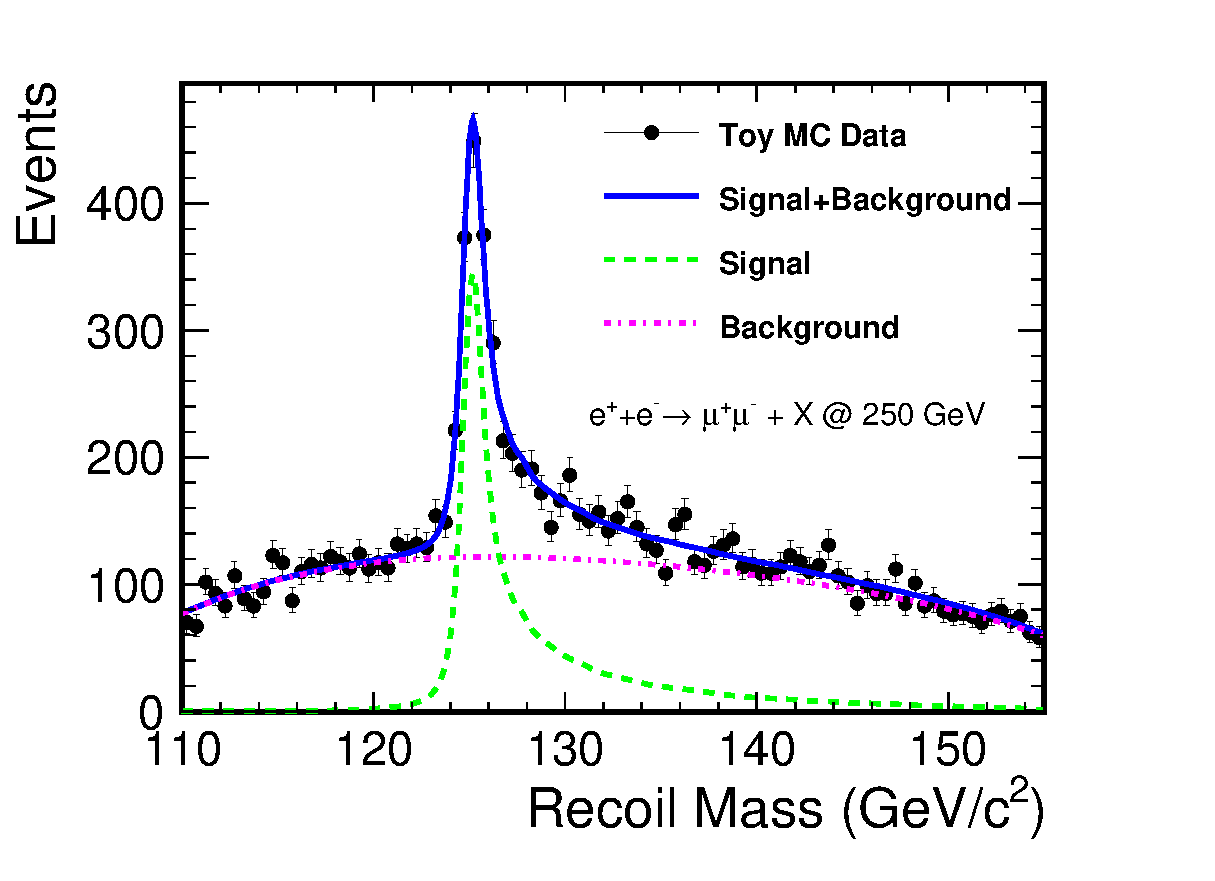
\includegraphics[width=0.85\hsize]{chapters/figures/RecoilMassLep250.eps}
\end{center}
  \caption{Recoil mass spectrum against
 $Z\to\mu^+\mu^-$ for signal $e^+e^-\to Zh$ and SM background 
  at 250 GeV \cite{Yan:2016xyx}.}
  \label{fig:RecoilMassLep250}
\end{figure}

\subsubsection{$\sigma_{\nu\bar{\nu}h}$ and $\sigma_{eeh}$}
[$W$-fusion and $Z$-fusion analyses, Fig.~\ref{fig:vvHbb}, to be filled]
\begin{figure}
%\begin{center}
\begin{tabular}[c]{c}
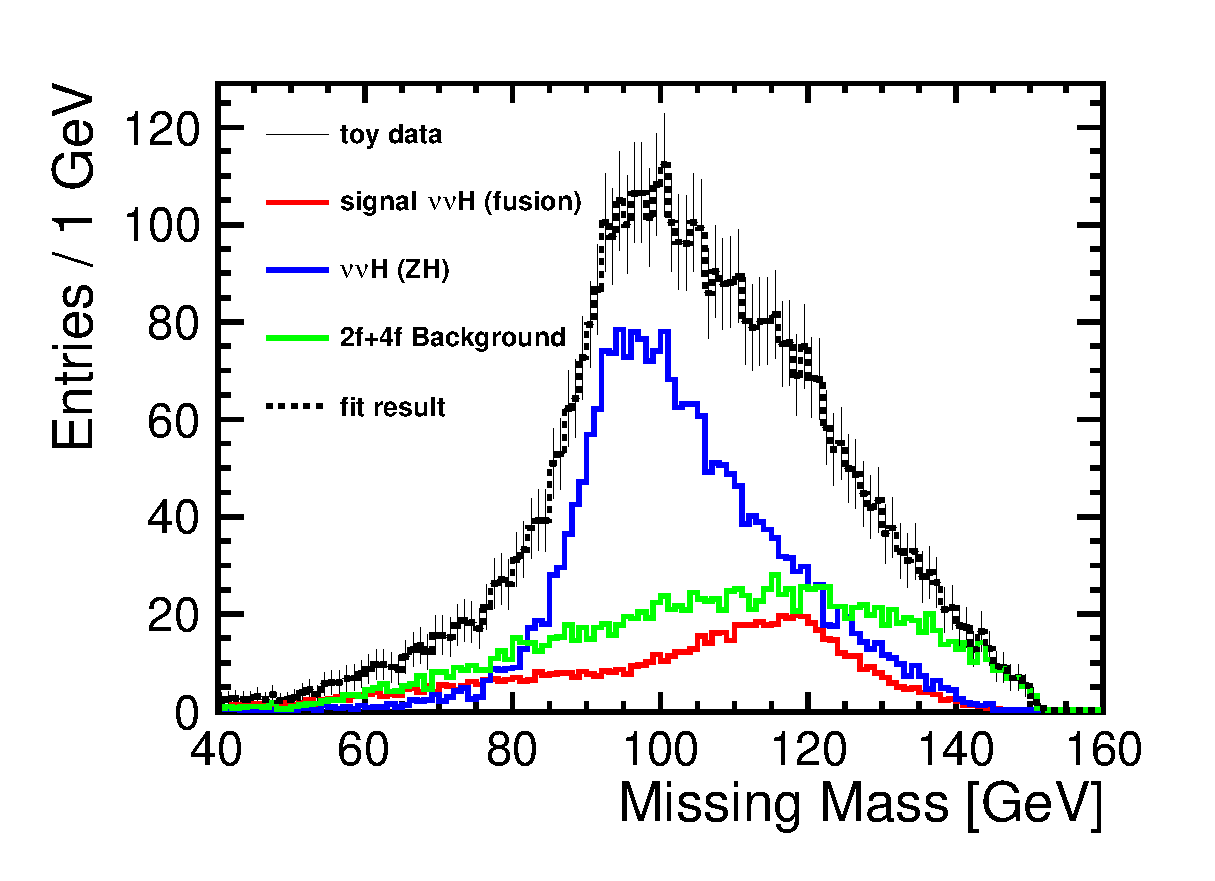
\includegraphics[width=0.85\hsize]{chapters/figures/vvH_MissingMass250.eps} \\
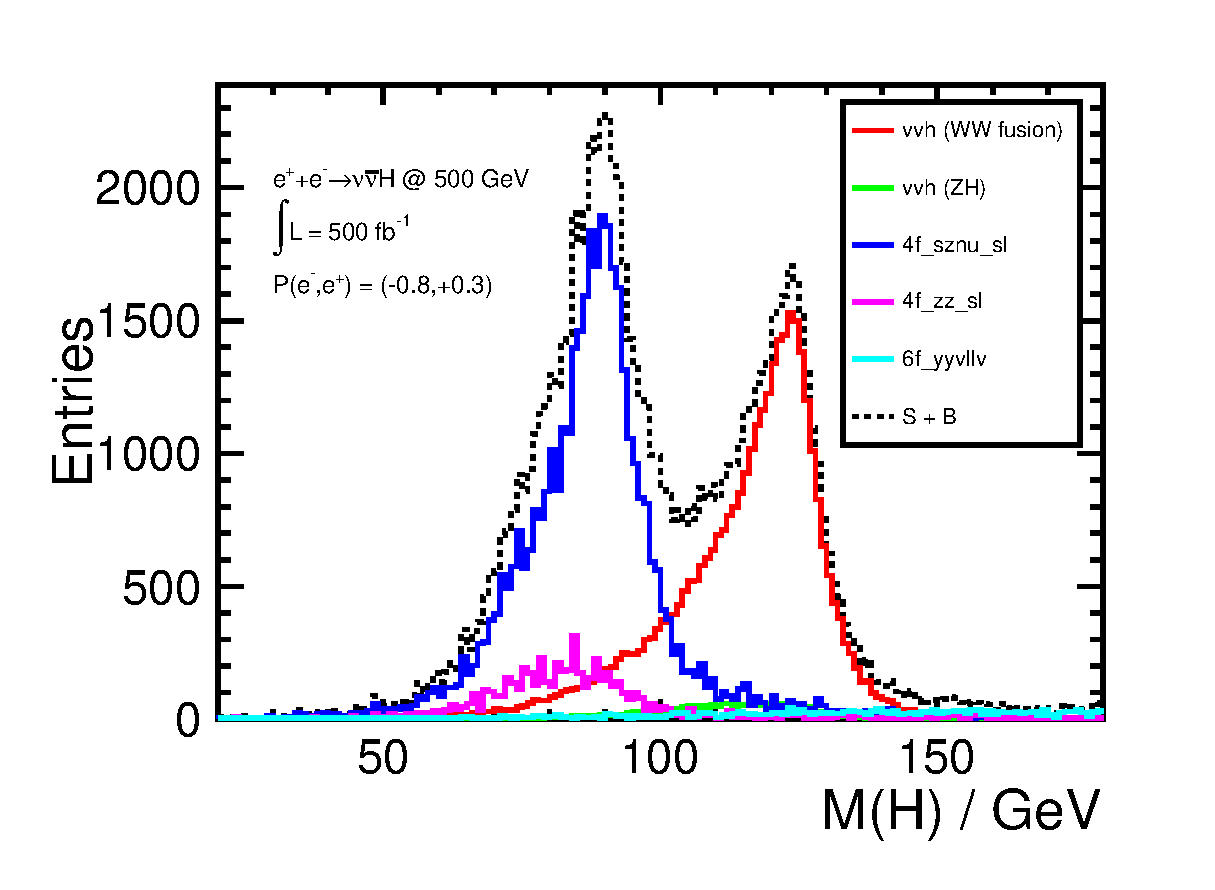
\includegraphics[width=0.85\hsize]{chapters/figures/vvH_MassH500.eps}
\end{tabular}
%\end{center}
  \caption{Missing mass spectrum (upper) and Higgs mass spectrum (lower) 
  for the signal $e^+e^-\to\nu\bar\nu h, h\to b \bar{b}$ and the SM background 
  at 250 GeV and 500 GeV respectively \cite{H2bb1,H2bb2}.}
  \label{fig:vvHbb}
\end{figure}

\subsubsection{$\mathrm{BR}(h\to b\bar{b}/c\bar{c}/gg)$}
[Fig.~\ref{fig:qqHbbccgg250}, to be filled]
\begin{figure*}
\begin{center}
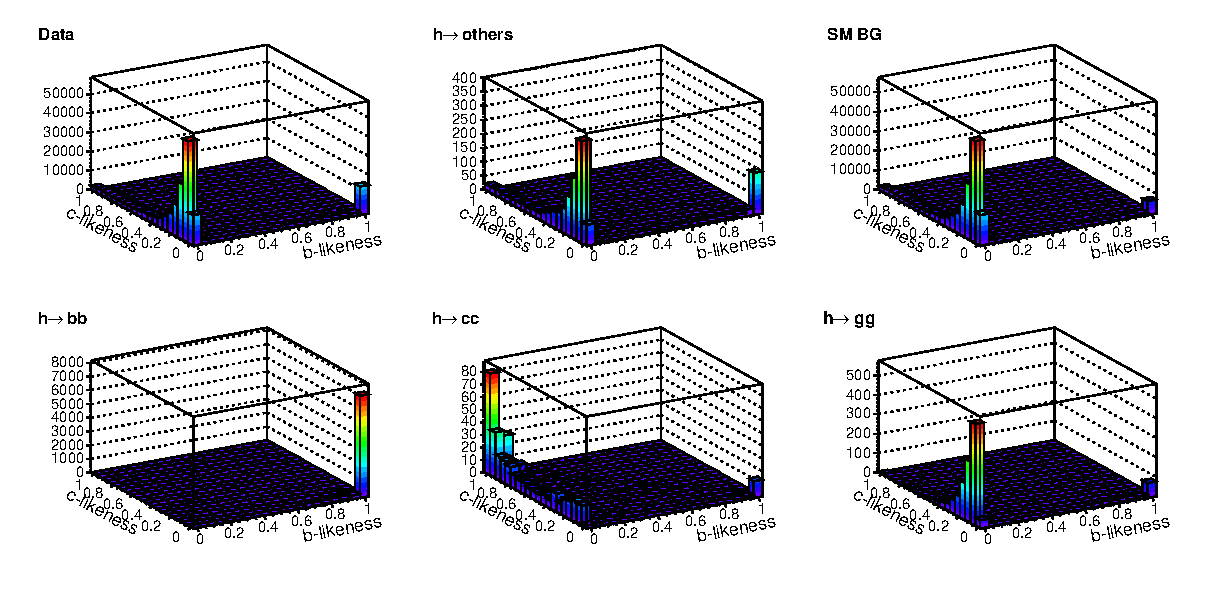
\includegraphics[width=0.85\hsize]{chapters/figures/qqh_bbccgg_template_250.eps}
\end{center}
  \caption{Template of b-likeliness versus c-likeness for signal $h\to b\bar{b}/c\bar{c}/gg$
  (bottom left/middle/right),
and for all events / $h\to others$ / SM background (top left/middle/right).}
  \label{fig:qqHbbccgg250}
\end{figure*}

\subsubsection{$\mathrm{BR}(h\to WW^*/ZZ^*)$}
[Fig.~\ref{fig:vvHWW500}, to be filled]
\begin{figure}
\begin{center}
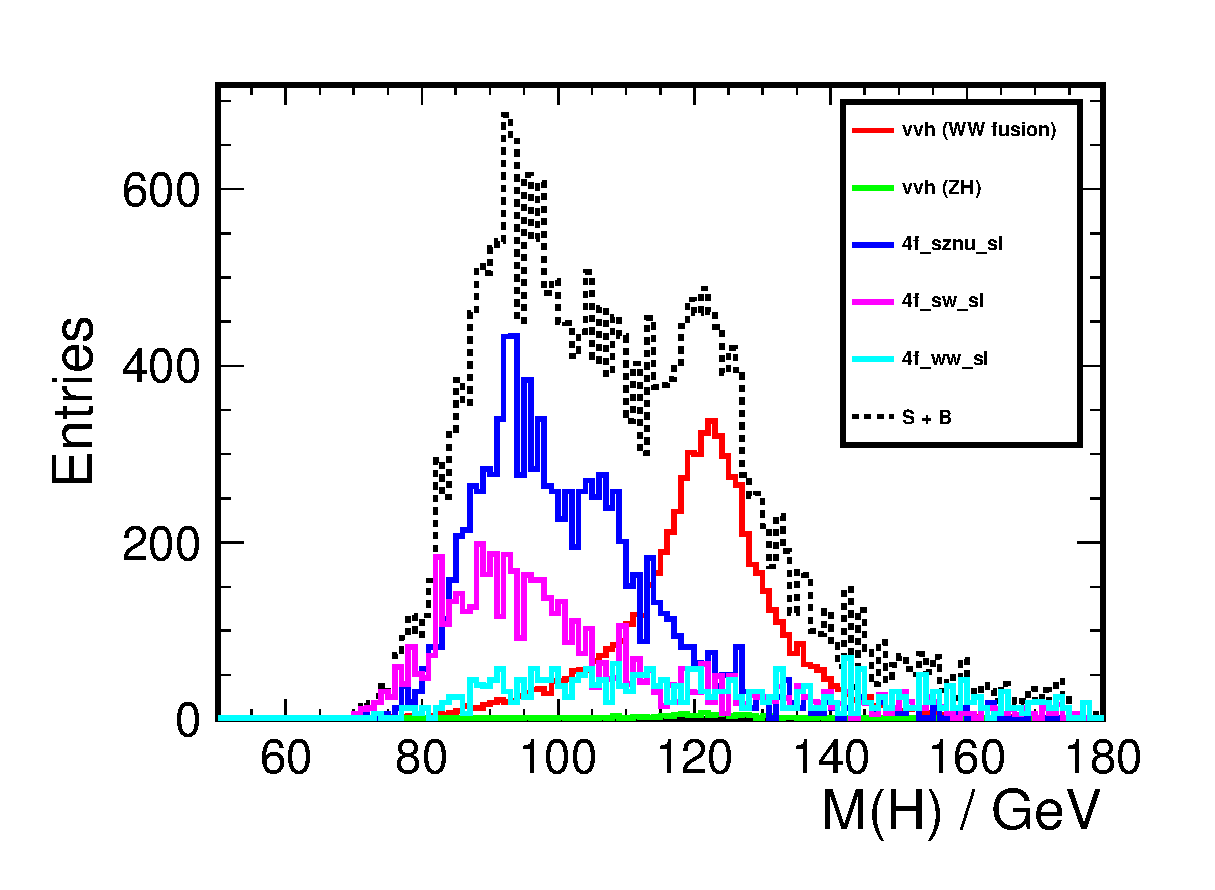
\includegraphics[width=0.85\hsize]{chapters/figures/vvH_WW4j500_MassH.eps}
\end{center}
  \caption{Higgs mass spectrum for the signal $e^+e^-\to\nu\bar\nu h, h\to WW^{*}$
  and $WW^{*}\to 4-jets$, and the SM background 
  at 500 GeV \cite{H2WW500}.}
  \label{fig:vvHWW500}
\end{figure}

\subsubsection{$\mathrm{BR}(h\to \tau^+\tau^-/\mu^+\mu^-)$}
[Fig.~\ref{fig:qqHtautau250}, to be filled]
\begin{figure}
\begin{center}
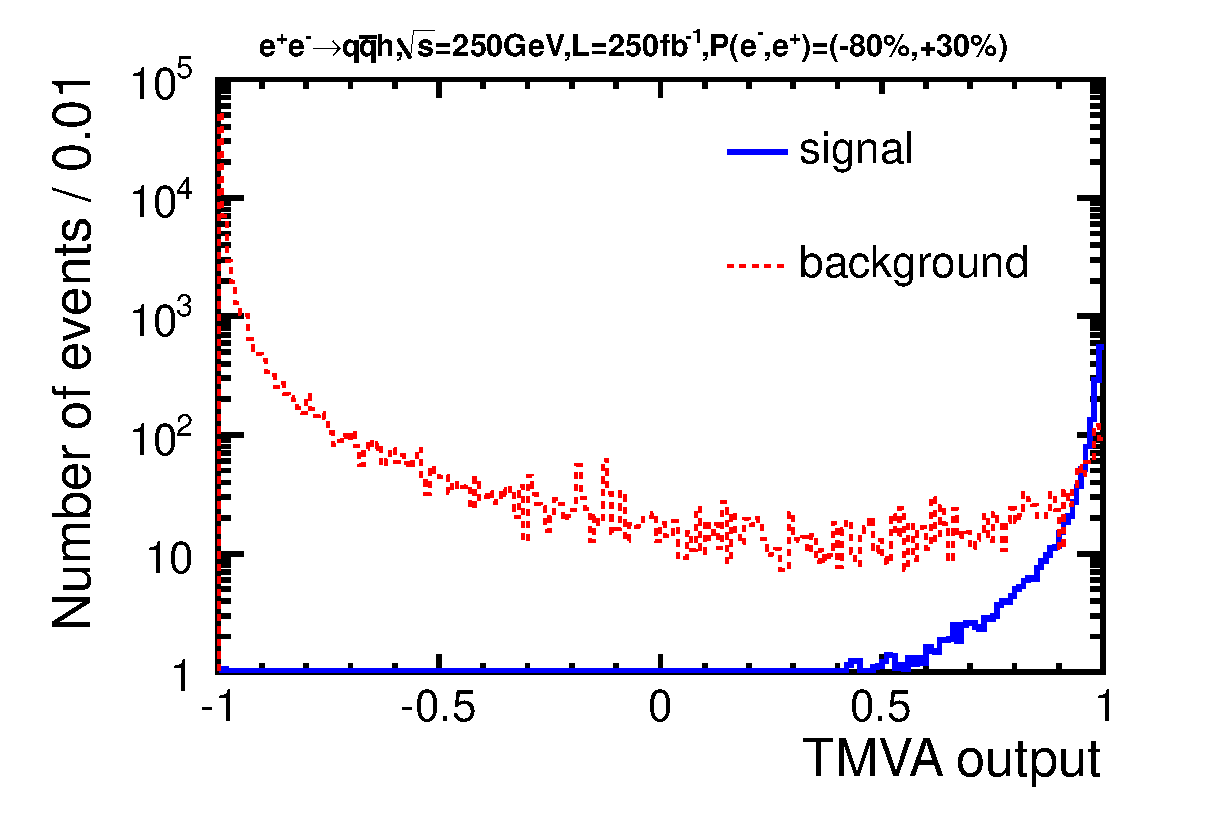
\includegraphics[width=0.85\hsize]{chapters/figures/ZH_qqtautau250_TMVA.eps}
\end{center}
  \caption{MVA output for the signal $e^+e^-\to q\bar{q} h, h\to\tau^+\tau^-$
 and the SM background at 250 GeV \cite{H2tautau250}.}
  \label{fig:qqHtautau250}
\end{figure}

\subsubsection{$\mathrm{BR}(h\to \mathrm{invisible/exotic})$}
[invisible analysis, Fig.\ref{fig:qqHinv250}, to be filled]
\begin{figure}
\begin{center}
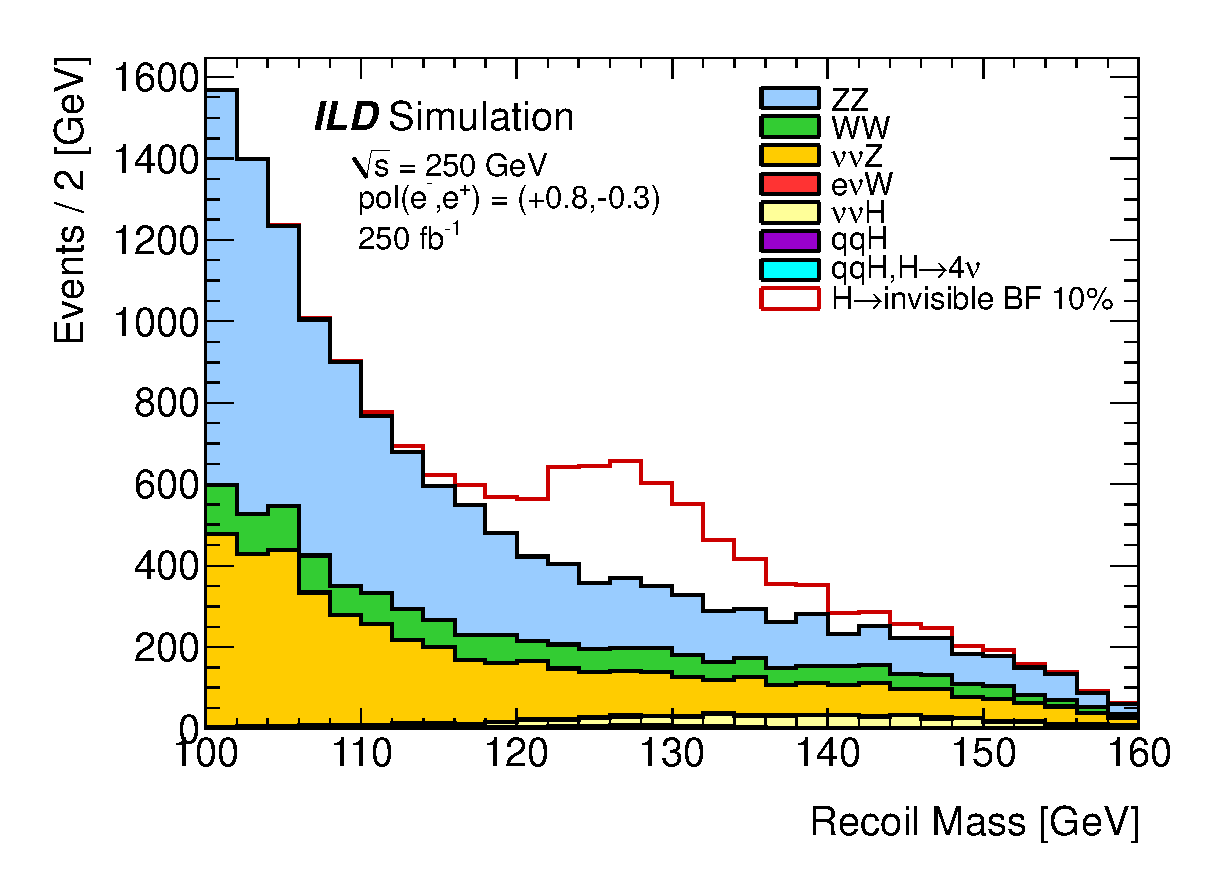
\includegraphics[width=0.85\hsize]{chapters/figures/ZH_qqinv250_right.eps}
\end{center}
  \caption{Recoil mass spectrum against
 $Z\to q\bar{q}$ for signal $e^+e^-\to Zh, h\to invisible$ assuming $BR(h\to invisible)=10\%$
  and SM background  at 250 GeV \cite{H2inv250}.}
  \label{fig:qqHinv250}
\end{figure}


\subsubsection{Higgs CP Properties}
[Fig.~\ref{fig:qqHtautauCP}, to be filled]
\begin{figure}
\begin{tabular}[c]{c}
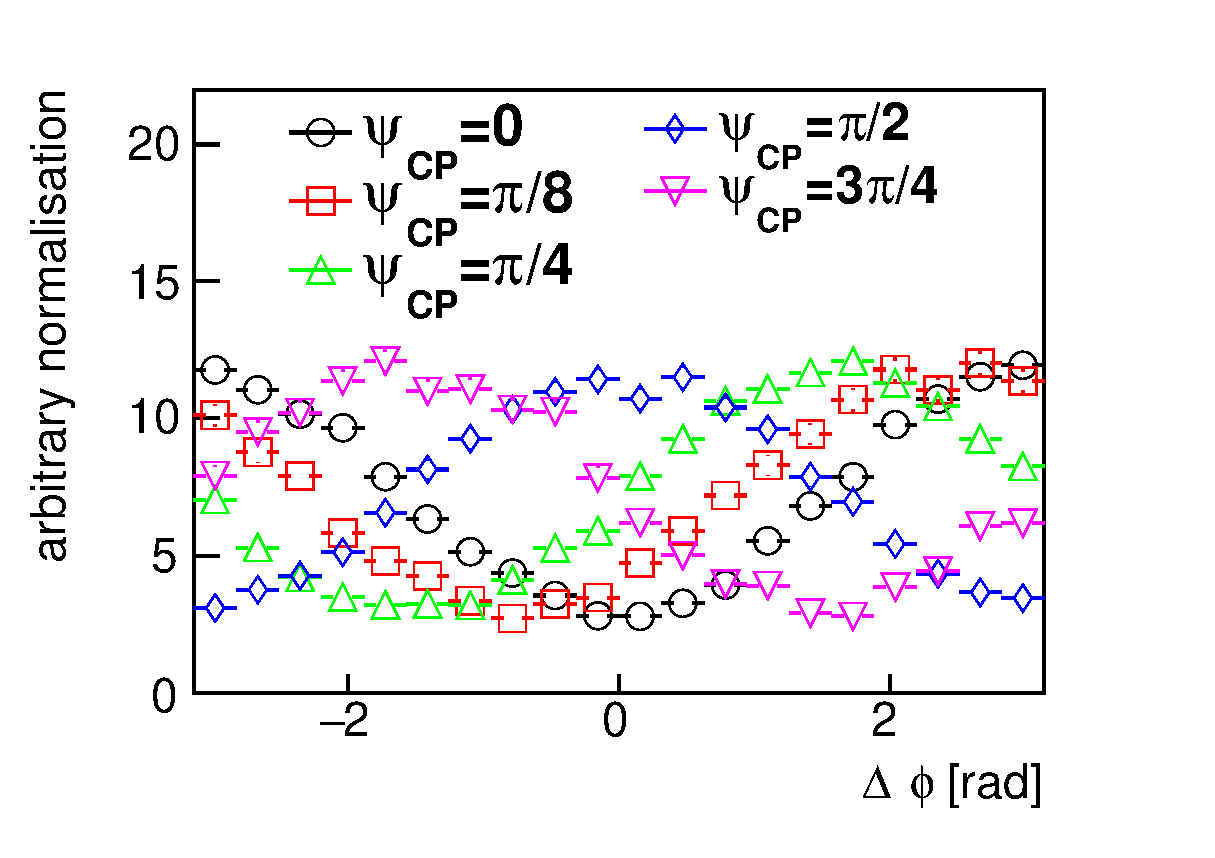
\includegraphics[width=0.85\hsize]{chapters/figures/ZH_qqtautau250_CP1.eps} \\
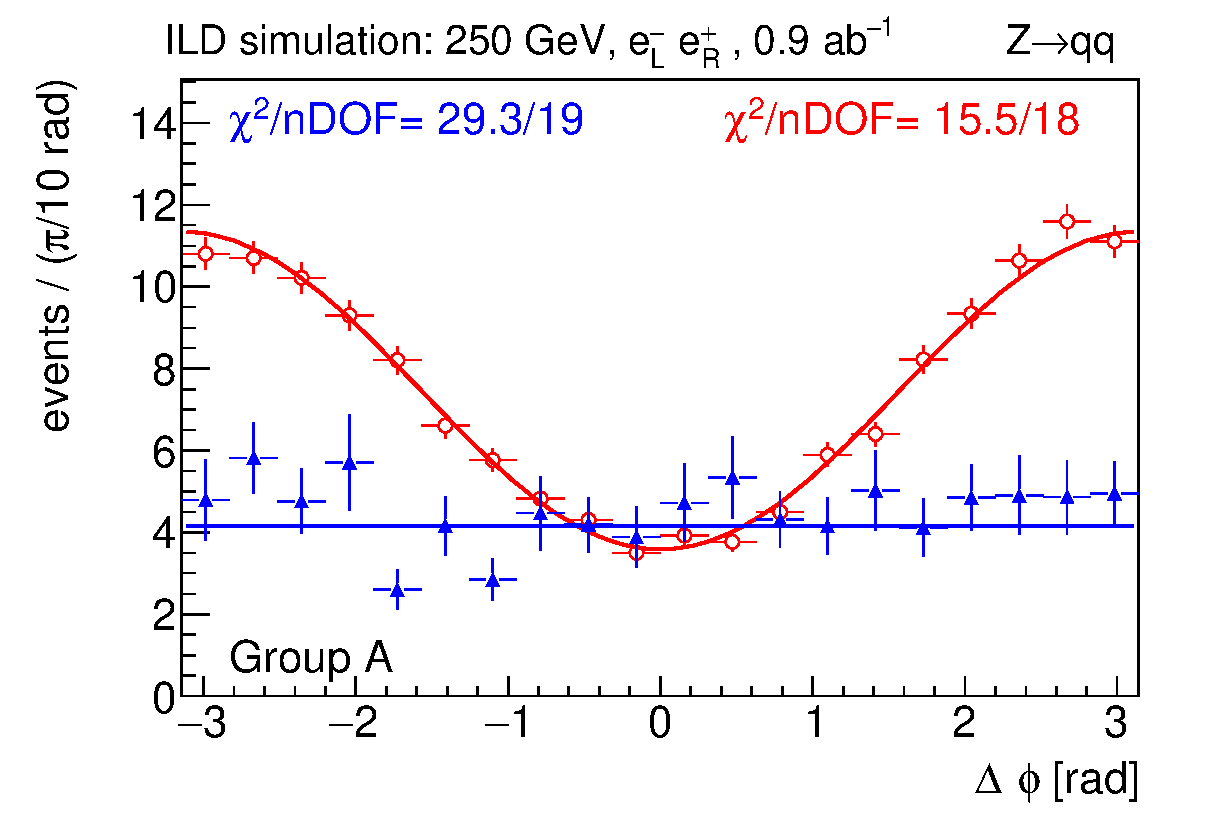
\includegraphics[width=0.85\hsize]{chapters/figures/ZH_qqtautau250_CP2.eps}
\end{tabular}
  \caption{Upper: $\Delta\phi$ distributions at MC Truth level for different 
  values of $\Phi_{CP}$ for the signal $e^+e^-\to q\bar{q} h, h\to\tau^+\tau^-$ at 250 GeV;
  Lower: reconstructed $\Delta\phi$ distributions after all cuts in the dominant category
  for the SM signal (in red) and the SM background (blue) respectively \cite{H2tautauCP}.}
  \label{fig:qqHtautauCP}
\end{figure}


\subsubsection{Angular Analyses for Anomalous $HVV$ Couplings}
[Fig.~\ref{fig:ZHanomHVV1} and~\ref{fig:ZHanomHVV2}, to be filled]
\begin{figure}
\begin{tabular}[c]{c}
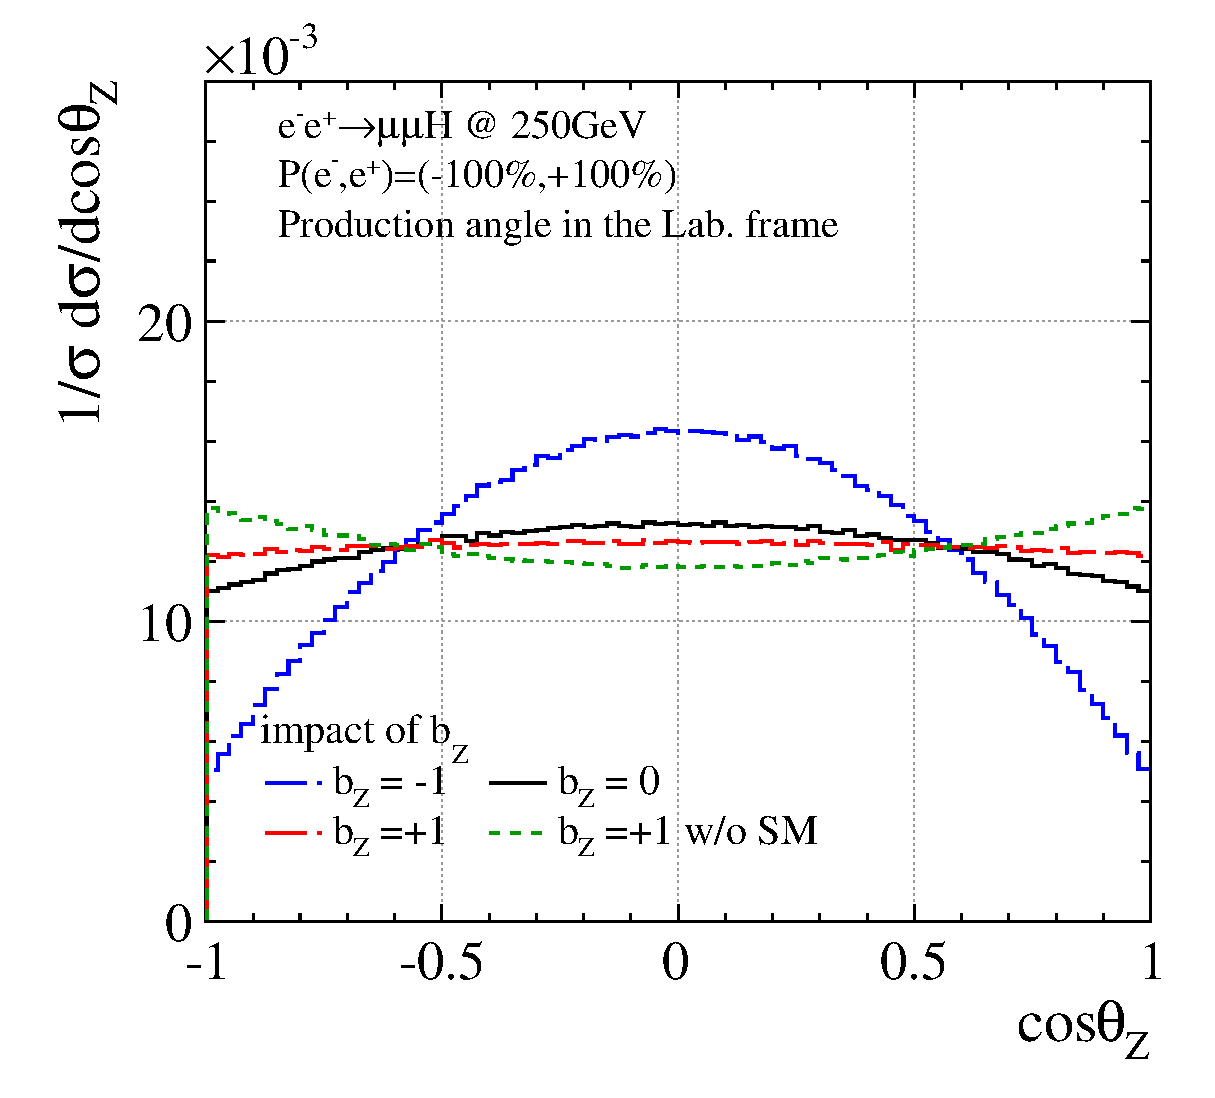
\includegraphics[width=0.85\hsize]{chapters/figures/ZH_anomHVV250_b.eps} \\
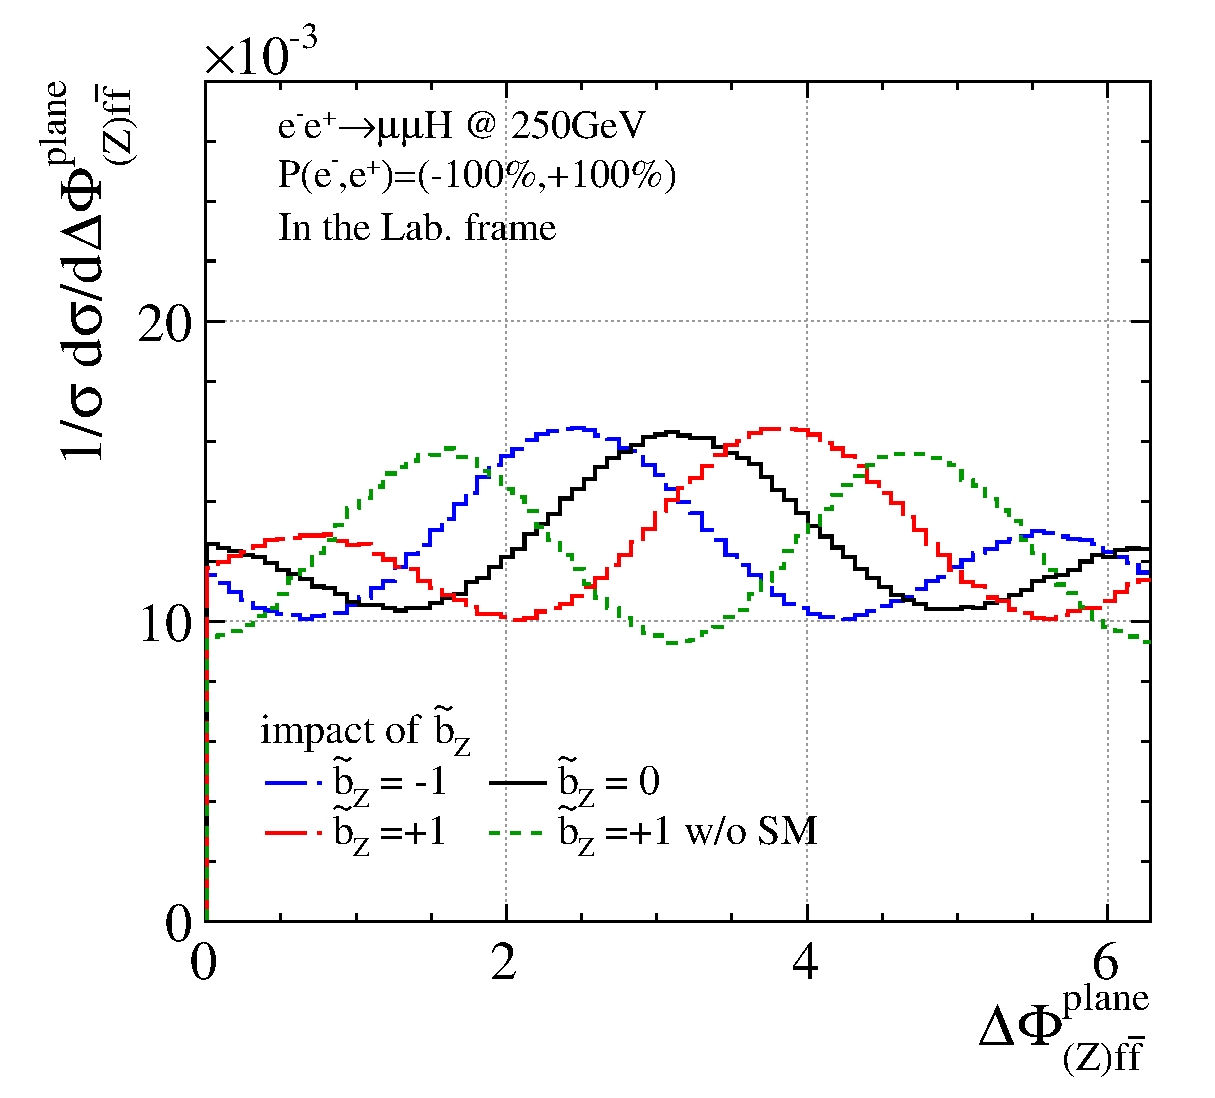
\includegraphics[width=0.85\hsize]{chapters/figures/ZH_anomHVV250_bt.eps} 
\end{tabular}
  \caption{Upper (lower): $\cos\theta_Z$ ($\Delta\Phi$) distributions at MC Truth level for different 
  values of anomalous coupling $b$ ($\tilde{b}$) 
  for the signal $e^+e^-\to \mu^+\mu^- h, h\to everthing$ at 250 GeV;
  \cite{anomHVV}.}
  \label{fig:ZHanomHVV1}
\end{figure}

\begin{figure*}
\begin{center}
\includegraphics[width=0.85\hsize]{chapters/figures/ZH_anomHVV_ab.eps}
\end{center}
  \caption{68\% and 95\% C.L. contour plots for fitted parameter $a$ versus $b$ at 250 GeV (left)
  and 500 GeV (right);
  \cite{anomHVV}.}
  \label{fig:ZHanomHVV2}
\end{figure*}


\subsection{Analyses of four-fermion final states} 
%\subsection{Analyses of $e^+e^- \to W^+W^-$} 
%\label{subsec:ew_WWana}

The analysis of four-fermion processes, e.g.\ from $W$-pair production, but also 
 $Z$-boson pairs and single-boson processes, plays a key role in the ILC physics program.  As discussed in Sec.~\ref{subsec:phys_WW}, constraints on triple gauge couplings (TGCs) are an important input to the dim-6 EFT-based interpretation of Higgs precision measurements introduced in Sec.~\ref{subsec:phys_eft}. Prospects for this type of analysis have been intensely studied in full detector simulation (c.f.\ Sec.~\ref{sec:software}), however only at center-of-mass energies of at least 500\,GeV. In this section, we will start out by summarizing these detailed studies, and then proceed to their recent extrapolations to a center-of-mass energy of 250\,GeV.


\subsubsection{Full Simulation Analyses of TGCs}
\label{subsubsec:ew_fullsimww}
The prospects for probing charged TGCs at the ILC have been studied in full, geant4-based simulation of the ILD detector concept at $\sqrt{s}=$500\,GeV~\cite{Marchesini:94888} in the context of the ILD Letter of Intent~\cite{Abe:2010aa} and at $\sqrt{s}=$1\,TeV~\cite{Rosca:2016hcq} as a benchmark for the ILD Detailed Baseline Design (Vol 4 ILC TDR~\cite{Behnke:2013lya}). Both analyses focused on the channel $e^+e^- \to W^+ W^- \to qql\nu$, $l=e, \mu$ and followed a similar, cut-based selection approach. Thereby they exploit the known initial state for a full kinematic reconstruction of both $W$ bosons, under consideration of optional photon radiation collinear to the beam direction.
Neither the case $l=\tau$, nor the fully hadronic mode, nor contributions from single-$W$ production were included at the time. Especially the fully hadronic mode will profit substantially from the recent advances in reconstructing the jet charge with the ILD detector, c.f.\ Sec.~\ref{subsec:ew_ffana}, in order to determine the charges of the $W$ boson candidates.

\begin{figure*}[]
\centerline{
\includegraphics[width=0.5\linewidth]{./chapters/figures/ep+30em-80SUMCosThetaWPRE}
\includegraphics[width=0.5\linewidth]{./chapters/figures/ep+30em-80resolutioncostheta}
}
\caption{Left: Reconstructed polar angle distribution $\cos\theta_{W}$ of the $W^-$ boson candidates for signal and SM background events before the application of the final selection cut $\cos\theta_{W} >$ -0.95. Right: relative deviation of the reconstructed $\cos\theta_{W}$ from the MC truth value $\cos\theta_{W}^\mathrm{T}$. Both from~\cite{Marchesini:94888}.}\label{fig:WW_costheta}
\end{figure*}

Figure~\ref{fig:WW_costheta} shows one of the final observables sensitive to anomalous TGCs,
namely the cosine of the polar angle of the $W^-$ boson, $\cos\theta_{W}$, which is reconstructed from the hadronically decaying $W$ boson. The left part of the figure illustrates the high purity of the selection which ranges between 85\% and 95\%, depending on whether  $WW \to qq\tau \nu$ is considered as background or not. The right panel shows relative deviation of the reconstructed $\cos\theta_{W}$ from MC truth, indicating a resolution of better than 0.5\%.
 
In the 500\,GeV analysis, no pile-up from $\gamma \gamma \to$ low $p_t$ hadrons was considered, which has, at $\sqrt{s}=$500\,GeV, an expectation value of 1.2 events per bunch crossing, c.f.\ Sec.~\ref{sec:software}.
This type of background was considered, however, in the TGC study at 1\,TeV, where its expectation value increases to 4.1 pile-up events per bunch crossing. Figure~\ref{fig:WW_overlayremoval} shows the impact of these pile-up events on the reconstructed hadronic $W$-boson mass without (``Durham'') and with (``Kt'') application of suitable suppression algorithms (see Sec~\ref{subsec:higgs_common} for a detailed description of the algorithm). It can be seen that the residual effect is small even at 1\,TeV, where the number of pile-up events is expected to be nearly four times higher than at 500\,GeV.

\begin{figure}
	\centering
		\includegraphics[width=0.95\linewidth]{./chapters/figures/wwjeting.pdf}
		
	\caption{Reconstructed mass of the hadronically decaying $W$ boson at $\sqrt{s}=$1\,TeV without pile-up compared to the situation with pile-up in absence (``Durham'') or presence (``Kt'') of a mitigation strategy in the analysis. From~\cite{Rosca:2016hcq}. 
	}
	\label{fig:WW_overlayremoval}
\end{figure}

Both full-simulation studies used only three out of five possible angular distributions which could provide sensitivity to TGCs: besides the production angle of the $W^-$, the two angles describing the direction of the decay lepton in the restframe of its mother $W$ were considered in a five-parameter fit based on MC templates. The free parameters of the fit were the three TGCs $ g^Z_1$, $\kappa_\gamma$ and $\lambda_\gamma$ as well as the absolute values of the electron and positron beam polarisations. With this approach, statistical uncertainties of about $6$-$7 \cdot 10^{-4}$ were obtained for all three couplings for an integrated luminosity of 500\,fb$^{-1}$ at $\sqrt{s}=$500\,GeV, shared equally between all four beam polarisation configurations.
In the context of the 500\,GeV analysis a thorough evaluation of the systematic errors was performed. It was found at the time that uncertainties on the selection efficiencies of signal and background of 0.2\% and 1\%, respectively, would lead to systematic effects in the same order of magnitude as the statistical uncertainty for 500\,fb$^{-1}$.

A recent study dedicated to a global fit of total and differential cross sections of various SM processes sensitive to TGCs and/or beam polarisation has shown, however, that a much better control of systematic effects can be achieved --- provided that {\em both} beams are polarised~\cite{bib:PhDRobert, Fujii:2018mli}.  

The full simulation study at $\sqrt{s}=$1\,TeV, following the same fitting approach, found statistical uncertainties of about $2$-$3 \cdot 10^{-4}$ for all three TGCs for an integrated luminosity of 1000\,fb$^{-1}$. The effect of different sharings of the luminosity between the four polarisation sign combinations on the TGC precisions were found to be minor. 

\subsubsection{Extrapolation of TGC prospects to 250\,GeV}

While extensive studies of $WW$ production exist at higher center-of-mass energies, no complete analysis based on full detector simulation is available yet for $\sqrt{s}=$250\,GeV. Nevertheless substantial progress has been made in various important aspects which have been incorporated in
an extrapolation~\cite{Fujii:2017vwa} based on a) the previously discussed full-simulation studies at 500\,GeV~\cite{Marchesini:94888} and 1\,TeV~\cite{Rosca:2016hcq} and b) the actual LEP results at $\sim$ 200\,GeV~\cite{Schael:2004tq}:
\begin{itemize}
\item As discussed in Sec.~\ref{subsec:phys_WW}, the sensitivity of measured cross sections to the TGCs depends on the center-of-mass energy as $s/m_W^2$.
\item Naively, the statistical uncertainties on measured cross sections scale as $1/\sqrt{\sigma \L}$. However at higher center-of-mass energies, the $W$ bosons are more and more boosted into the forward direction due to increasing amount of ISR and beamstrahlung. Therefore the experimental acceptance decreases for higher $\sqrt{s}$. A correction factor for this effect has been derived~\cite{Karl:2017let} from a comparison of the full detector simulation studies at 500\,GeV and 1\,TeV.
\item The dependence on the sharing of luminosity between the four different polarisation configurations was found minor~\cite{Rosca:2016hcq} and therefore no corrections for differences in the assumptions of the full simuation studies w.r.t.\ the H20 running scenario (c.f.\ Sec.~\ref{subsec:runscen_pol}) were applied.
\item The improved treatment of systematic uncertainties based on a nuisance parameter technique in a global fit to many observables and datasets explored in~\cite{bib:PhDRobert} was assumed, which leads to a constant ratio between systematic and statistical uncertainties up to luminosities of at least 2\,ab$^{-1}$.
\item The full simulation studies were found to be limited their MC-based, binned fit of 3D-template histograms. The relative improvement expected when including the fully hadronic channel and when exploiting all five sensitive angles (production angle of one of the $W$ bosons plus decay angles of both $W$ bosons, see e.g.\ Fig. 5.16 in~\cite{Marchesini:94888} for an ilustration) in an unbinned fit~\cite{Barklow:1995sk}, or, equivalently, when applying an optimal observable technique~\cite{Diehl:1997ft, Diehl:2002nj}, was estimated in a parton-level study to be a factor 2.4 in the case of $ g^Z_1$, and a factor of 1.9 for the other two couplings.
\item Since none of the ILC full-simulation studies evaluated the precisions for single-coupling fits, i.e.\ when fixing the other two anomalous couplings to 0 as done in hadron collider studies,
the corresponding LEP2 results~\cite{Schael:2004tq} were extrapolated up in center-of-mass energy,
and then the minimum of this extrapolation and of the 3-coupling extrapolation from ILC studies was taken.
\end{itemize}

The results of this procedure are displayed in Tab.~\ref{table:ew_tgc} and Figs~\ref{fig:TGC_1par} and~\ref{fig:TGC_3par} in comparison with the LEP2 and LHC results as well as HL-LHC projections, where applicable. In case of the single-parameter fits, the 250\,GeV stage of the ILC will improve the precision on $ g^Z_1$ and $\kappa_\gamma$ by factors of 5 and 30 w.r.t\ to HL-LHC, while the projections for $\lambda_\gamma$ are comparable. The loss in precision when fitting all three couplings simultaneously to ILC data is minor, and the resulting precisions are used as input for the EFT-based Higgs coupling fit discussed in Sec.~\ref{subsec:higgs_lhcilc}. Actually it has been shown in the past that even the 14 complex couplings in the most general parametrisation of triple gauge boson vertices, including e.g.\ $CP$ violating contributions, can be determined simulataneously at future $e^+e^-$ linear colliders when both beams are polarised and all polarisation configurations, including transverse polarisation, are exploited~\cite{Diehl:2002nj}.

\begin{table}
\begin{center}
  \begin{tabular} {|l|c||c|c|c||c|c|c||}
    \hline
 &   &  \multicolumn{3}{|c||}{total error ($\times 10^{-4}$) } & \multicolumn{3}{c||}{correlation} \\
    \hline
    Exp & $N_{par}$ & $ g^Z_1$  & $\kappa_\gamma$ & $\lambda_\gamma$ & $g^Z_1\ \kappa_\gamma$ &  $g^Z_1\ \lambda_\gamma$  & $\kappa_\gamma\ \lambda_\gamma$  \\
    \hline
    LEP~2     & 3     &  $516$  & $618$  & $376$  & -0.17 & -0.62 & -0.15 \\
    ILC~250   & 3        & $4.4$ & $5.7$ & $4.2$ & 0.63 & 0.48 & 0.35 \\
    \hline
    LEP~2     & 1     & $300$ & $626$ & $292$ & -- & -- & -- \\
    LHC      & 1     & $319$ & $1077$ & $198$ & -- & -- & -- \\
    HL-LHC   & 1      & $19$ & $160$ & $4$ & -- & -- & -- \\
    ILC~250   & 1       & $3.7$ & $5.7$ & $3.7$ & -- & -- & -- \\
    \hline

\end{tabular}
  \caption{TGC precisions for LEP~2, Run1 at LHC, HL-LHC and the ILC at $\sqrt{s}=250$~GeV with 2000~fb$^{-1}$ luminosity (ILC~250). The LEP~2 result is from ALEPH~\cite{Schael:2004tq} at  $\sqrt{s}\approx 200$~ GeV with
    0.68~fb$^{-1}$.  The LHC result is from ATLAS\cite{Aad:2014mda} at $\sqrt{s}=7$~TeV with 4.6~fb$^{-1}$.  The HL-LHC estimate is from a 2013 overview of HL-LHC physics~\cite{bib:HLLHCMoenig}. From~\cite{Fujii:2017vwa}.}
\label{table:ew_tgc}
\end{center}
\end{table}

\begin{figure}
	\centering
		\includegraphics[width=0.95\linewidth]{./chapters/figures/TGC_LHCsep.pdf}
		
	\caption{Comparison of the reachable TGC precision from single parameter fits: ILC~\cite{bib:TGC_EPS17}, final results from LEP combined from ALEPH, L3 and OPAL results~\cite{bib:LEPTGC} and the LHC TGC limits for $\sqrt{s} = 8$\,TeV data and an integrated luminosity of $\mathcal{L} = 20.3$\ifb and  $\mathcal{L} = 19.4$\ifb for ATLAS and CMS, respectively~\cite{bib:LHCTGC}. 
	}
	\label{fig:TGC_1par}
\end{figure}

\begin{figure}
	\centering
		\includegraphics[width=0.95\linewidth]{./chapters/figures/TGC_Multi.pdf}
		
	\caption{Comparison of the reachable TGC precision from a simultaneous fit of all three parameters: ILC~\cite{bib:TGC_EPS17} and final results from LEP combined from ALEPH, L3 and OPAL results~\cite{bib:LEPTGC}. No comparable hadron collider results are available.
	}
	\label{fig:TGC_3par}
\end{figure}

\subsubsection{$W$ Mass Measurement at 250\,GeV}
\label{subsubsec:ew_mw}
The analysis of $W^+W^- \to qql\nu$ discussed in the previous sections, as well as the study of single-$W$ events also offer an excellent setting for the measurement of the $W$ mass. As discussed in Sec.~\ref{subsec:phys_ff}, the available statistics at the 250\,GeV ILC will be about a factor of 2000 larger than at LEP2, which makes it obvious that a pure consideration of statistical uncertainties is meaningless. While the studies discussed in Sec.~\ref{subsubsec:ew_fullsimww} showed that this kind of events can be selected with high efficiency and purity, a careful extrapolation of the systematic uncertainties of previous measurements is therefore much more instructive than the evaluation of the statistical uncertainty from full detector simulation.
Apart from a scan of the production threshold, kinematic reconstruction of $W$ pair events 
and calorimetric comparison of hadronic $W$ and  $Z$ decays in single-boson events are the most promising techniques, which are described in detail in~\cite{Freitas:2013xga, Wilson:2016tto}.   With a combination of methods and considering advances in theory as well as in the performance of the detectors the systematic limit has been estimated as 2.4\,MeV. This is expected to be reached already at the 250\,GeV stage of the ILC. Additional datasets at higher center-of-mass energies 
could then provide independent information in order to cross-check and constrain systematic effects.


\subsection{Analyses of two-fermion final states}
\begin{figure*}
       \includegraphics[width=0.45\linewidth]{./chapters/figures/basymmetry-final-left.pdf}
       \llap{\shortstack{%
                       \includegraphics[clip, trim=0cm 0cm 1.8cm 1.7cm, scale=.15]{./chapters/figures/zoom-final.pdf}\\
                       \rule{0ex}{0.67in}%
               }
               \rule{2.2in}{0ex}}
        \hspace{0.2cm}       
        \includegraphics[width=0.45\linewidth]{./chapters/figures/basymmetry-final-right.pdf}
	\caption{Polar angle distribution $\cos{\theta_b}$ of generated $b$-quarks and final reconstructed 
         $b$-jets including any SM  background remaining after event selection. 
         Left:  $P(e^+,e^-)=(+100\%,-100\%)$ with a zoom of the region with negative 
         $\cos{\theta_b}$.
         Right: $P(e^+,e^-)=(-100\%,+100\%)$. From~\cite{Bilokin:2017lco}.  }
	\label{fig:ffbar_basym}
\end{figure*}


\begin{figure}
	\centering
	\includegraphics[width=0.95\columnwidth]{./chapters/figures/final-graph-ild.pdf}
	%	\includegraphics[width=0.95\linewidth]{./chapters/figures/ilc-precision-ild.png}
	\caption{\sl  Comparison of the LEP measurements to the expected 
                  precision at the ILC. The results of the ILC correspond to the 
                  integrated luminosity of $\mathcal{L}_I = 500$\,fb$^{-1}$ to be collected 
                   at $\sqrt{s} = 250$\,GeV before the luminosity upgrade. Final results for the
                  full 250\,GeV dataset would improve the precision further by about a factor of 2.
                   From~\cite{Bilokin:2017lco}.}
	\label{fig:LEPILCResult_3}
\end{figure}


\subsection{Systematic Errors}

The estimates shown in~\ref{tab:higgserrors} are only for statistical uncertainties. In the global fit,
following systematic uncertainties are imposed:
\begin{itemize}
\item 0.1\% from theory; applied to all $\sigma$ and $\sigma\cdot BR$ Higgs measurements.
\item 0.1\% from luminosity and beam polarization; 
applied to all $\sigma$ and $\sigma\cdot BR$ Higgs measurements.
\item 0.3\%$\times\sqrt{250/L}$ ($L$ for integrated luminosity in fb$^{-1}$) for b-tagging efficiency; 
applied to $\sigma\cdot BR(h\to b\bar{b})$ measurements.
\end{itemize}
Note in addition to the systematic uncertainties for Higgs measurement, 
in the global fit we also include systematic 
uncertainties for TGCs measurement; introduced in Section VIII.



\subsection{Estimation for Future Improvements}








As elaborated in the previous section, all the estimates for Higgs measurements shown in
~\ref{tab:higgserrors} are based on available full simulation studies, which are performed using the analysis
techniques known at present. These estimates are clearly too
conservative in the sense that we have not been able to exploit all
useful signal channels.  In addition, analysts working closely with
the data are always able to invent algorithms to that more cleverly
optimize the data that is actually collected.   The projected
uncertainties  quoted here and
here and in Sec.~\ref{subsec:global:elements} do not take advantage of
these  likely improvements.

Since the formal estimates of the performance of HL-LHC given in the
HL-LHC Yellow Report~\cite{Cepeda:2019klc} do take into account
improvements in systematic uncertainties that are anticipated but not
yet realised, it seems to us reasonable to define also for ILC an
optimistic scenario with improved performance.   We use this scenario
to compare to the results of Ref.~\cite{Cepeda:2019klc} in the manner
explained in Sec.~\ref{subsec:higgs:ilclhc}.   This scenario, which we 
refer to as ``S2'' in that discussion, includes the following
improvements in the analysis just described.  In all cases, these
improvements are under study by our group using our full simulation
tools
and are  suggested, if not yet validated, by our current results: 
\begin{itemize}
\item 10\% improvement in signal efficiency of the  jet clustering algorithm.
\item 20\% improvement in the performance of the  flavor tagging algorithm. 
\item 20\% improvement in statistics by including more signal channels
  in  $\sigma_{Zh}\cdot BR(h\to WW*)$. 
\item a factor of 10 improvement in the precision electroweak input
  $A_{\ell}$ thorugh the measurment of $e^+e^-\to\gamma Z$ with
  polarized beams at 250~GeV.
\end{itemize}


\subsection{Comparison of the ILC Higgs capability with 
HL-LHC projections}
\input{Supporting-documents/chapters/higgs_lhcilc.tex}




\section{\label{sec:ew}Physics Simulations: Electroweak Production of 2- and 4-Fermion Final States }


  5 pages J. List
  

% Intro, connection to Physics Case
The precision studies of the Higgs boson described in the previous section receive important and complementary support from analyses of 2- and 4-fermion final states which do not directly involve Higgs bosons, but our well-known SM gauge bosons --- or potentially their yet to be discovered siblings. In this section, some of the key examples introduced in Sec.~\ref{subsec:phys_WW}  will be discussed in more detail, highlighting the level of realism on which the projections are based. 


\subsection{Analyses of $e^+e^- \to W^+W^-$} 
\label{subsec:ew_WWana}
%\subsection{Analyses of $e^+e^- \to W^+W^-$} 
%\label{subsec:ew_WWana}

The analysis of four-fermion processes, e.g.\ from $W$-pair production, but also 
 $Z$-boson pairs and single-boson processes, plays a key role in the ILC physics program.  As discussed in Sec.~\ref{subsec:phys_WW}, constraints on triple gauge couplings (TGCs) are an important input to the dim-6 EFT-based interpretation of Higgs precision measurements introduced in Sec.~\ref{subsec:phys_eft}. Prospects for this type of analysis have been intensely studied in full detector simulation (c.f.\ Sec.~\ref{sec:software}), however only at center-of-mass energies of at least 500\,GeV. In this section, we will start out by summarizing these detailed studies, and then proceed to their recent extrapolations to a center-of-mass energy of 250\,GeV.


\subsubsection{Full Simulation Analyses of TGCs}
\label{subsubsec:ew_fullsimww}
The prospects for probing charged TGCs at the ILC have been studied in full, geant4-based simulation of the ILD detector concept at $\sqrt{s}=$500\,GeV~\cite{Marchesini:94888} in the context of the ILD Letter of Intent~\cite{Abe:2010aa} and at $\sqrt{s}=$1\,TeV~\cite{Rosca:2016hcq} as a benchmark for the ILD Detailed Baseline Design (Vol 4 ILC TDR~\cite{Behnke:2013lya}). Both analyses focused on the channel $e^+e^- \to W^+ W^- \to qql\nu$, $l=e, \mu$ and followed a similar, cut-based selection approach. Thereby they exploit the known initial state for a full kinematic reconstruction of both $W$ bosons, under consideration of optional photon radiation collinear to the beam direction.
Neither the case $l=\tau$, nor the fully hadronic mode, nor contributions from single-$W$ production were included at the time. Especially the fully hadronic mode will profit substantially from the recent advances in reconstructing the jet charge with the ILD detector, c.f.\ Sec.~\ref{subsec:ew_ffana}, in order to determine the charges of the $W$ boson candidates.

\begin{figure*}[]
\centerline{
\includegraphics[width=0.5\linewidth]{./chapters/figures/ep+30em-80SUMCosThetaWPRE}
\includegraphics[width=0.5\linewidth]{./chapters/figures/ep+30em-80resolutioncostheta}
}
\caption{Left: Reconstructed polar angle distribution $\cos\theta_{W}$ of the $W^-$ boson candidates for signal and SM background events before the application of the final selection cut $\cos\theta_{W} >$ -0.95. Right: relative deviation of the reconstructed $\cos\theta_{W}$ from the MC truth value $\cos\theta_{W}^\mathrm{T}$. Both from~\cite{Marchesini:94888}.}\label{fig:WW_costheta}
\end{figure*}

Figure~\ref{fig:WW_costheta} shows one of the final observables sensitive to anomalous TGCs,
namely the cosine of the polar angle of the $W^-$ boson, $\cos\theta_{W}$, which is reconstructed from the hadronically decaying $W$ boson. The left part of the figure illustrates the high purity of the selection which ranges between 85\% and 95\%, depending on whether  $WW \to qq\tau \nu$ is considered as background or not. The right panel shows relative deviation of the reconstructed $\cos\theta_{W}$ from MC truth, indicating a resolution of better than 0.5\%.
 
In the 500\,GeV analysis, no pile-up from $\gamma \gamma \to$ low $p_t$ hadrons was considered, which has, at $\sqrt{s}=$500\,GeV, an expectation value of 1.2 events per bunch crossing, c.f.\ Sec.~\ref{sec:software}.
This type of background was considered, however, in the TGC study at 1\,TeV, where its expectation value increases to 4.1 pile-up events per bunch crossing. Figure~\ref{fig:WW_overlayremoval} shows the impact of these pile-up events on the reconstructed hadronic $W$-boson mass without (``Durham'') and with (``Kt'') application of suitable suppression algorithms (see Sec~\ref{subsec:higgs_common} for a detailed description of the algorithm). It can be seen that the residual effect is small even at 1\,TeV, where the number of pile-up events is expected to be nearly four times higher than at 500\,GeV.

\begin{figure}
	\centering
		\includegraphics[width=0.95\linewidth]{./chapters/figures/wwjeting.pdf}
		
	\caption{Reconstructed mass of the hadronically decaying $W$ boson at $\sqrt{s}=$1\,TeV without pile-up compared to the situation with pile-up in absence (``Durham'') or presence (``Kt'') of a mitigation strategy in the analysis. From~\cite{Rosca:2016hcq}. 
	}
	\label{fig:WW_overlayremoval}
\end{figure}

Both full-simulation studies used only three out of five possible angular distributions which could provide sensitivity to TGCs: besides the production angle of the $W^-$, the two angles describing the direction of the decay lepton in the restframe of its mother $W$ were considered in a five-parameter fit based on MC templates. The free parameters of the fit were the three TGCs $ g^Z_1$, $\kappa_\gamma$ and $\lambda_\gamma$ as well as the absolute values of the electron and positron beam polarisations. With this approach, statistical uncertainties of about $6$-$7 \cdot 10^{-4}$ were obtained for all three couplings for an integrated luminosity of 500\,fb$^{-1}$ at $\sqrt{s}=$500\,GeV, shared equally between all four beam polarisation configurations.
In the context of the 500\,GeV analysis a thorough evaluation of the systematic errors was performed. It was found at the time that uncertainties on the selection efficiencies of signal and background of 0.2\% and 1\%, respectively, would lead to systematic effects in the same order of magnitude as the statistical uncertainty for 500\,fb$^{-1}$.

A recent study dedicated to a global fit of total and differential cross sections of various SM processes sensitive to TGCs and/or beam polarisation has shown, however, that a much better control of systematic effects can be achieved --- provided that {\em both} beams are polarised~\cite{bib:PhDRobert, Fujii:2018mli}.  

The full simulation study at $\sqrt{s}=$1\,TeV, following the same fitting approach, found statistical uncertainties of about $2$-$3 \cdot 10^{-4}$ for all three TGCs for an integrated luminosity of 1000\,fb$^{-1}$. The effect of different sharings of the luminosity between the four polarisation sign combinations on the TGC precisions were found to be minor. 

\subsubsection{Extrapolation of TGC prospects to 250\,GeV}

While extensive studies of $WW$ production exist at higher center-of-mass energies, no complete analysis based on full detector simulation is available yet for $\sqrt{s}=$250\,GeV. Nevertheless substantial progress has been made in various important aspects which have been incorporated in
an extrapolation~\cite{Fujii:2017vwa} based on a) the previously discussed full-simulation studies at 500\,GeV~\cite{Marchesini:94888} and 1\,TeV~\cite{Rosca:2016hcq} and b) the actual LEP results at $\sim$ 200\,GeV~\cite{Schael:2004tq}:
\begin{itemize}
\item As discussed in Sec.~\ref{subsec:phys_WW}, the sensitivity of measured cross sections to the TGCs depends on the center-of-mass energy as $s/m_W^2$.
\item Naively, the statistical uncertainties on measured cross sections scale as $1/\sqrt{\sigma \L}$. However at higher center-of-mass energies, the $W$ bosons are more and more boosted into the forward direction due to increasing amount of ISR and beamstrahlung. Therefore the experimental acceptance decreases for higher $\sqrt{s}$. A correction factor for this effect has been derived~\cite{Karl:2017let} from a comparison of the full detector simulation studies at 500\,GeV and 1\,TeV.
\item The dependence on the sharing of luminosity between the four different polarisation configurations was found minor~\cite{Rosca:2016hcq} and therefore no corrections for differences in the assumptions of the full simuation studies w.r.t.\ the H20 running scenario (c.f.\ Sec.~\ref{subsec:runscen_pol}) were applied.
\item The improved treatment of systematic uncertainties based on a nuisance parameter technique in a global fit to many observables and datasets explored in~\cite{bib:PhDRobert} was assumed, which leads to a constant ratio between systematic and statistical uncertainties up to luminosities of at least 2\,ab$^{-1}$.
\item The full simulation studies were found to be limited their MC-based, binned fit of 3D-template histograms. The relative improvement expected when including the fully hadronic channel and when exploiting all five sensitive angles (production angle of one of the $W$ bosons plus decay angles of both $W$ bosons, see e.g.\ Fig. 5.16 in~\cite{Marchesini:94888} for an ilustration) in an unbinned fit~\cite{Barklow:1995sk}, or, equivalently, when applying an optimal observable technique~\cite{Diehl:1997ft, Diehl:2002nj}, was estimated in a parton-level study to be a factor 2.4 in the case of $ g^Z_1$, and a factor of 1.9 for the other two couplings.
\item Since none of the ILC full-simulation studies evaluated the precisions for single-coupling fits, i.e.\ when fixing the other two anomalous couplings to 0 as done in hadron collider studies,
the corresponding LEP2 results~\cite{Schael:2004tq} were extrapolated up in center-of-mass energy,
and then the minimum of this extrapolation and of the 3-coupling extrapolation from ILC studies was taken.
\end{itemize}

The results of this procedure are displayed in Tab.~\ref{table:ew_tgc} and Figs~\ref{fig:TGC_1par} and~\ref{fig:TGC_3par} in comparison with the LEP2 and LHC results as well as HL-LHC projections, where applicable. In case of the single-parameter fits, the 250\,GeV stage of the ILC will improve the precision on $ g^Z_1$ and $\kappa_\gamma$ by factors of 5 and 30 w.r.t\ to HL-LHC, while the projections for $\lambda_\gamma$ are comparable. The loss in precision when fitting all three couplings simultaneously to ILC data is minor, and the resulting precisions are used as input for the EFT-based Higgs coupling fit discussed in Sec.~\ref{subsec:higgs_lhcilc}. Actually it has been shown in the past that even the 14 complex couplings in the most general parametrisation of triple gauge boson vertices, including e.g.\ $CP$ violating contributions, can be determined simulataneously at future $e^+e^-$ linear colliders when both beams are polarised and all polarisation configurations, including transverse polarisation, are exploited~\cite{Diehl:2002nj}.

\begin{table}
\begin{center}
  \begin{tabular} {|l|c||c|c|c||c|c|c||}
    \hline
 &   &  \multicolumn{3}{|c||}{total error ($\times 10^{-4}$) } & \multicolumn{3}{c||}{correlation} \\
    \hline
    Exp & $N_{par}$ & $ g^Z_1$  & $\kappa_\gamma$ & $\lambda_\gamma$ & $g^Z_1\ \kappa_\gamma$ &  $g^Z_1\ \lambda_\gamma$  & $\kappa_\gamma\ \lambda_\gamma$  \\
    \hline
    LEP~2     & 3     &  $516$  & $618$  & $376$  & -0.17 & -0.62 & -0.15 \\
    ILC~250   & 3        & $4.4$ & $5.7$ & $4.2$ & 0.63 & 0.48 & 0.35 \\
    \hline
    LEP~2     & 1     & $300$ & $626$ & $292$ & -- & -- & -- \\
    LHC      & 1     & $319$ & $1077$ & $198$ & -- & -- & -- \\
    HL-LHC   & 1      & $19$ & $160$ & $4$ & -- & -- & -- \\
    ILC~250   & 1       & $3.7$ & $5.7$ & $3.7$ & -- & -- & -- \\
    \hline

\end{tabular}
  \caption{TGC precisions for LEP~2, Run1 at LHC, HL-LHC and the ILC at $\sqrt{s}=250$~GeV with 2000~fb$^{-1}$ luminosity (ILC~250). The LEP~2 result is from ALEPH~\cite{Schael:2004tq} at  $\sqrt{s}\approx 200$~ GeV with
    0.68~fb$^{-1}$.  The LHC result is from ATLAS\cite{Aad:2014mda} at $\sqrt{s}=7$~TeV with 4.6~fb$^{-1}$.  The HL-LHC estimate is from a 2013 overview of HL-LHC physics~\cite{bib:HLLHCMoenig}. From~\cite{Fujii:2017vwa}.}
\label{table:ew_tgc}
\end{center}
\end{table}

\begin{figure}
	\centering
		\includegraphics[width=0.95\linewidth]{./chapters/figures/TGC_LHCsep.pdf}
		
	\caption{Comparison of the reachable TGC precision from single parameter fits: ILC~\cite{bib:TGC_EPS17}, final results from LEP combined from ALEPH, L3 and OPAL results~\cite{bib:LEPTGC} and the LHC TGC limits for $\sqrt{s} = 8$\,TeV data and an integrated luminosity of $\mathcal{L} = 20.3$\ifb and  $\mathcal{L} = 19.4$\ifb for ATLAS and CMS, respectively~\cite{bib:LHCTGC}. 
	}
	\label{fig:TGC_1par}
\end{figure}

\begin{figure}
	\centering
		\includegraphics[width=0.95\linewidth]{./chapters/figures/TGC_Multi.pdf}
		
	\caption{Comparison of the reachable TGC precision from a simultaneous fit of all three parameters: ILC~\cite{bib:TGC_EPS17} and final results from LEP combined from ALEPH, L3 and OPAL results~\cite{bib:LEPTGC}. No comparable hadron collider results are available.
	}
	\label{fig:TGC_3par}
\end{figure}

\subsubsection{$W$ Mass Measurement at 250\,GeV}
\label{subsubsec:ew_mw}
The analysis of $W^+W^- \to qql\nu$ discussed in the previous sections, as well as the study of single-$W$ events also offer an excellent setting for the measurement of the $W$ mass. As discussed in Sec.~\ref{subsec:phys_ff}, the available statistics at the 250\,GeV ILC will be about a factor of 2000 larger than at LEP2, which makes it obvious that a pure consideration of statistical uncertainties is meaningless. While the studies discussed in Sec.~\ref{subsubsec:ew_fullsimww} showed that this kind of events can be selected with high efficiency and purity, a careful extrapolation of the systematic uncertainties of previous measurements is therefore much more instructive than the evaluation of the statistical uncertainty from full detector simulation.
Apart from a scan of the production threshold, kinematic reconstruction of $W$ pair events 
and calorimetric comparison of hadronic $W$ and  $Z$ decays in single-boson events are the most promising techniques, which are described in detail in~\cite{Freitas:2013xga, Wilson:2016tto}.   With a combination of methods and considering advances in theory as well as in the performance of the detectors the systematic limit has been estimated as 2.4\,MeV. This is expected to be reached already at the 250\,GeV stage of the ILC. Additional datasets at higher center-of-mass energies 
could then provide independent information in order to cross-check and constrain systematic effects.



\subsection{Analyses of $e^+e^- \to f \bar{f}$}
\label{subsec:ew_ffana}
\begin{figure*}
       \includegraphics[width=0.45\linewidth]{./chapters/figures/basymmetry-final-left.pdf}
       \llap{\shortstack{%
                       \includegraphics[clip, trim=0cm 0cm 1.8cm 1.7cm, scale=.15]{./chapters/figures/zoom-final.pdf}\\
                       \rule{0ex}{0.67in}%
               }
               \rule{2.2in}{0ex}}
        \hspace{0.2cm}       
        \includegraphics[width=0.45\linewidth]{./chapters/figures/basymmetry-final-right.pdf}
	\caption{Polar angle distribution $\cos{\theta_b}$ of generated $b$-quarks and final reconstructed 
         $b$-jets including any SM  background remaining after event selection. 
         Left:  $P(e^+,e^-)=(+100\%,-100\%)$ with a zoom of the region with negative 
         $\cos{\theta_b}$.
         Right: $P(e^+,e^-)=(-100\%,+100\%)$. From~\cite{Bilokin:2017lco}.  }
	\label{fig:ffbar_basym}
\end{figure*}


\begin{figure}
	\centering
	\includegraphics[width=0.95\columnwidth]{./chapters/figures/final-graph-ild.pdf}
	%	\includegraphics[width=0.95\linewidth]{./chapters/figures/ilc-precision-ild.png}
	\caption{\sl  Comparison of the LEP measurements to the expected 
                  precision at the ILC. The results of the ILC correspond to the 
                  integrated luminosity of $\mathcal{L}_I = 500$\,fb$^{-1}$ to be collected 
                   at $\sqrt{s} = 250$\,GeV before the luminosity upgrade. Final results for the
                  full 250\,GeV dataset would improve the precision further by about a factor of 2.
                   From~\cite{Bilokin:2017lco}.}
	\label{fig:LEPILCResult_3}
\end{figure}


% bb, $\mu\mu$, $\tau\tau$


  

\section{\label{sec:global}Global Fit to Higgs Boson Couplings and Effective Field Theory Parameters}

  

\subsection{Elements of the fit to Higgs couplings from Effective Field Theory}
\label{subsec:global:elements}


In this section, we make use of the simulation results presented in
Secs.~\ref{sec:higgs} and \ref{sec:ew} to present projections for the
uncertainties in Higgs boson couplings that will be obtained from the
ILC both at this 250~GeV stage and after running at 500~GeV according
to the plan presented in Sec.~\ref{sec:runscenarios}.   

To extract
Higgs boson couplings from measurements, we will use the method of
Effective Field Theory (EFT) sketched in Sec.~\ref{subsec:phys_eft}.
This method has been explained in full technical  detail in
\cite{Barklow:2017suo,Barklow:2017awn}.
Here we will present an overview of the EFT analysis, supplying those 
technical details that are relevant to the evaluation of our fitting procedure.

[ stuff goes here ] 

[forward reference to the importance of polarization]

From this analysis, we derive the projected uncertainties on Higgs
couplings shown in Tab.~\ref{tab:ILCHiggs}.  We emphasize that the
analysis leading to these projections is completely model-independent,
in the sense that all models of new physics describable either by the
addition  of local operators to the SM EFT (for heavy new particles)
or by the addition of invisible and exotic Higgs decays (for light new
particles) are included.  These estimates give the
current state of our understanding of the ILC capabilities.  Given the
run plan and  detector designs described above, we have a high degree
of confidence that these estimated uncertainties will be achieved --
and, probably, surpassed -- in the realization of the ILC program.
The projections in the table are summarized in Fig.~\ref{fig:ILCmodelindep}.



%%%%%%%%%%%%%%%%
\begin{figure}
\begin{center}
\includegraphics[width=0.85\hsize]{chapters/figures/ModelindepSummary.pdf}
\caption{Projected Higgs boson coupling uncertainties for the ILC
  program at 250~GeV and an energy upgrade to 500~GeV, using the
  highly model-independent analysis presented in \cite{Fujii:2017vwa}. This
  analysis makes use of  data on $\ee\to W^+W^-$ in addition to Higgs
  boson observables and also incorporates projected LHC results, as described
  in the text.  These
values correspond to the  scenario S1* in Table~\ref{tab:ILCLHC}.}
\label{fig:ILCmodelindep}
\end{center}
\end{figure}
%%%%%%%%%%%%%%%%%%%%%%%%%%%%%%%%%%%%%%%%%%%%%%%%%%%%%%%%%%%%%%
%


\subsection{Systematic uncertainties and the importance of beam polarization for precision measurements at $\ee$  colliders}
\label{subsec:polarization}

% \subsection{Systematic uncertainties and the importance of beam polarization for precision measurements at $\ee$  colliders}
% \label{subsec:polarization}
% 
% % \subsection{Systematic uncertainties and the importance of beam polarization for precision measurements at $\ee$  colliders}
% \label{subsec:polarization}
% 
% \input{chapters/polarization.tex}

Beam polarization is considered as an essential ingredient of the ILC physics program because of three important advantages:
\begin{enumerate}
\item Suppression of backgrounds and enhancement of signals
\item Analysis of the chiral properties
\item Control of systematic uncertainties
\end{enumerate}
The first two items often (but not always!) apply to a large extent already when only electron polarisation is available. 
However for the third aspect, the positron polarisation is crucial in many cases --- in particular whenever the left-right asymmetry \ALR\ itself is the physics observable, like \eg\ for 2-fermion processes (see Sec.~\ref{subsec:ew_ffana}) or for the Higgs precision measurements (see Sec.~\ref{subsec:ew_WWana}).
All three aspects will be discussed and illustrated with concrete physics examples in the following subsections. 

A comprehensive review of the role of polarization with many more examples can be found in~\cite{MoortgatPick:2005cw}, and a recent discussion of positron polarization in particular in~\cite{Fujii:2018mli}. 

%%%%%%%%%%%%%%%%%%%%%%%%%%%%%%%%%%%%%%%%%%%%%%%%%%%%%%%%%%%%%%%%%%%%%%%%%%%%5

\subsubsection{Suppression of backgrounds and enhancement of signals} 
\label{subsubsec:pol:s_over_b}
Due to the chiral structure of the weak interaction, and especially since right-handed fermions form isospin-singlets and therefore don't participate in charged current interactions, every $e^+e^-$ cross section depends on the chirality of the incoming beam particles.  For any given polarization of the electron and positron beams, \Pem\ and \Pep, respectively, the polarised cross section is caluculated from the chiral cross sections in the following way:
\begin{eqnarray}
\sigma_{\Pem\Pep} &=& \frac{1}{4}\bigl\{
     (1+\Pem)(1+\Pep) \quad \sigmaRR  \nonumber \\
&& + (1-\Pem)(1-\Pep) \sigmaLL \nonumber \\
&& + (1+\Pem)(1-\Pep) \sigmaRL \nonumber \\ 
&& + (1-\Pem)(1+\Pep) \sigmaLR \bigr\},
\label{eq:pol:xsec}
\end{eqnarray}


For charged current $t$-channel processes, like $e^+e^- \to W^+W^-$, $e^+e^- \to \nu_e\bar{\nu}_e$ or Higgs production via $WW$ fusion, only the \sigmaLR\ contribution is allowed, so that their rate can be dialed up or down by a factor 17 for $\Pmp=(\pm 80\%,\mp 30\%)$ (36 for $\Pmp=(\pm 80\%,\mp 60\%)$) via the choice of the polarisation sign. 

For $s$-channel processes in the SM, including Higgsstrahlung, \sigmaLR\ and \sigmaRL\ contribute. In this case, Eqn~\ref{eq:pol:xsec} can be reduced to
\begin{equation}
 \sigma_{\Pem\Pep} = 2 \sigma_0 (\Leff/\mathcal{L}) \left[1 - \ALR \Peff \right]
\label{eq:pol:xsecschan}
\end{equation}
Here, $\sigma_0$ is the unpolarized cross section and \ALR\ 
the left-right asymmetry, defined in Eqn.~\ref{eq:defALR}. \Leff\ and \Peff\  
are the effective luminosity and polarization, respectively, defined as
\begin{equation}
\Peff= \frac{\Pem - \Pep}{1 - \Pep\Pem}
\label{eq:def-leff-peff}
\quad\mbox{\rm and }\quad
\Leff=\frac{1}{2}(1 -\Pep\Pem)\L
\end{equation}

In practice, for $\Pmp=(\pm 80\%,\mp 30\%)$, $\Peff = \pm 89\%$ and $\Leff = 62\% \mathcal{L}$, whereas for $\Pmp=(0,0)$ and , $\Peff = 0$ and $\Leff = 50\% \mathcal{L}$, since in half of the cases a left-handed electron will meet a left-handed positron --- for which the cross section for $s$-channel processes is zero. 

With \ALR = 0.151 for Higgsstrahlung, this means that the cross section for $\Pmp=(-80\%,+30\%)$ is 41\% larger than the unpolarised cross section, while it is
still 7\% larger than the unpolarised cross section for the opposite sign combination  $\Pmp=(+80\%,-30\%)$. Since, as we saw above, important background processes like $e^+e^- \to W^+W^-$ are strongly suppressed in this configuration, the $\Pmp=(+80\%,-30\%)$ gives comparable and in some cases even better results than the $\Pmp=(-80\%,+30\%)$ configuration. 

However the signal-to-background ratio ($S/B$ or $S/sqrt{B}$) cannot be maximized for all processes at the same time. But it is very important to realize that the combination of a high-$S/B$ data set with a low-$S/B$ data set is statistically {\em not} equivalent to taking 
the same amount of data with the average $S/B$, simply because significances don't add up linearly. Therefore the overall precision increases even if the total intergrated luminosity is split between ``optimal'' and ``non-optimal'' configurations. 

This is illustrated in Fig.~\ref{fig:polWIMPstat}, which compares the reach of the search for WIMP production in the mono-photon channel for different assumptions on luminosity and polarization (see Sec.~\ref{sec:searches} for a description of the analysis). It clearly shows the large increase in sensitivity for \Pmp=(+80\%, -30\%) w.r.t.\ the unpolarised case, and that the result for splitting the data on all four helicity configurations as forseen in the H20 running scenario, albeit completely dominated by the 1.6\,\iab\ collected with \Pmp=(+80\%, -30\%), is still probing significantly higher scales than the unpolarised case. Note that this figure omits all systematic uncertainties in order to highlight the statistical $S/B$ effect. 
\begin{figure}
\centering
\includegraphics[width=0.95\linewidth]{./chapters/figures/vector_noSystematics.pdf}
		
\caption{{\color{red}[Figure layout will be improved!]} Comparison of the reach of the search for WIMP production in the mono-photon channel for different assumptions on luminosity and polarization (see Sec.~\ref{sec:searches} for a description of the analysis)~\cite{Habermehl:417605}. Note that this plot is considering {\em statistical uncertainties only}. The corresponding comparison {\em including systematic uncertainties} is shown in Fig.~\ref{fig:polWIMPsys}.}
\label{fig:polWIMPstat}
\end{figure}

%%%%%%%%%%%%%%%%%%%%%%%%%%%%%%%%%%%%%%%%%%%%%%%%%%%%%%%%%%%%%%%%%%%%%%%%%%%%5

\subsubsection{Analysis of chiral properties} 
\label{subsubsec:pol:chiral}
Beam polarisation is essential to analyze the chiral structure of SM processes in search for deviations from a pure $V-A$ structure due to new physics contributions --- and, in case of a discovery of new particles at the LHC or the ILC itself, of these new particles and their interaction. The list of example applications is long and comprises for instance:
\begin{itemize}
\item Measurements fermion couplings in 2-fermion production: Beam polarisation is essential to disentangle the left- and right-handed couplings of each fermion species to the photon and the $Z$ boson, as discussed in Sec.~\ref{subsec:ew_ffana}. 
\item Measurements of triple gauge couplings: With both beams polarized and using various orientations of the polarisation vectors, all 14 complex couplings (thus 28 real parameters) of the most general Lagrangian for triple gauge vertices, including $CP$ violation, can be extracted simultaneously, as  discussed in Sec.~\ref{subsec:ew_WWana}.
\item Higgs coupling determination: The left-right asymmetry of the $ZH$ cross section has been found to be an important ingredient for constraining the full set of $CP$ conserving dimension-6 operators consistent with $SU(2) \times\ U(1)$ symmetry. This will be discussed in detail in Sec.~\ref{sec:global}.
\item Generic BSM effects: The chiral structure of physics beyond the SM is apriory not known - it could be similar to the SM or completely different. When parametrising new physics in terms of effective operators, the tensor structure of the operator immediately relates to the chiral cross sections: For instance the $s$-channel exchange of a vector mediator allows only for \sigmaLR\ and \sigmaRL\ by angular momentum conservation,
while the exchange of a scalar also has non-zero \sigmaLL\ and \sigmaRR. Since these
vanish in the SM, like-sign polarisation configurations are extremely sensitive to 
such types of new interactions. An example is e.g.\ the distinction between different WIMP models in the mono-photon channel, as discussed in Sec.~\ref{subsec:searches_monophoton}.
\end{itemize}  
% Many more applications can be found e.g.\ in~\cite{MoortgatPick:2005cw, Fujii:2018mli}. 

%%%%%%%%%%%%%%%%%%%%%%%%%%%%%%%%%%%%%%%%%%%%%%%%%%%%%%%%%%%%%%%%%%%%%%%%%%%%5

\subsubsection{Control of systematic uncertainties} 
\label{subsubsec:pol:systematics}

Last but not least, the redundancies provided by the combination of data sets with different beam polarization configurations are invaluable for the control of systematics uncertainties. Thereby it important to always have one more degree of freedom that (statistically) absolutely required: For physics measurements which do not aim at the analysis of a chiral structure, e.g.\ measurements of total unpolarised cross sections, two data sets with with different polarisations (e.g.\ $\Pmp=(\pm 80\%, \mp 30\%)$ or $\Pmp=(\pm 80\%, 0)$ often suffice to constrain the most important nuisance parameters. However if the chiral structure itself is among the observables, e.g.\ when measuring \ALR\ of 2-fermion processes or of Higgsstrahlung, one flip of the polarisation sign(s) is already contained in the observable itself, and thus a non-zero positron polarisation becomes essential to provide enough independent information to constrain nuisance parameters.

{\color{blue} Points to make here:
\begin{itemize}
\item Fast-helicity reversal creates of the systematic effects between data sets with different polarisations. Note that this does not apply for data sets with different center-of-mass energies, which are typically taken in different years, thus all effects from changes to the configuration, calibration or alignment of the detector and the accelerator do not correlate between such data sets.
\item In case of correlated uncertainties, the data sets with different polarisations serve mutually as control samples, allowing for large cancellations of systematic uncertainties. Plot from Robert's thesis Fig. 10.13. $\Rightarrow$ factor 2 on $WW$, factor 4 on $Z$.
\item Help of positron polarisation to control uncertainty on \ALR\ measurement: Digest of Tab 10.6 in Robert's thesis, make graphical version: w/o positron polarisation, uncertainties on \ALR\ increase by 2 factor 2 on $WW$ production and by a factor of $10$ on $s$-channel $Z$ exchange.
\item For ILC precisions, a residual polarisation of 0.25\% would already create a bias on cross sections and asymmetries when not allowed for as nuissance parameter $\to$ plot from Robert's thesis Fig 10.2
\item WIMP example: discuss Fig.~\ref{fig:polWIMPsys} The limit calculation uses a fractional event counting based on the 
energy spectrum of the photon. With larger WIMP masses, the maximum energy of the ISR photons becomes lower. At the highest WIMP masses, the signal-free part of the spectrum becomes large enough to also help to constrain the nuisance parameters and thus to limited the impact of the systematic uncertainties. This effect is visible in form of the ``bump'' in the limit curves near $M_X=220$\,GeV. In case of the unpolarised data set, the effect starts to become visible already from $M_X=150$\,GeV onwards. 
%The study includes a careful evaluation of the systematic uncertainties, comprising those on selection efficiencies, luminosity, beam energy (spectrum) and polarization as well as on the theoretical modelling of the background. 
\end{itemize}
}


\begin{figure}
\centering
\includegraphics[width=0.95\linewidth]{./chapters/figures/vector_withSystematics.pdf}
		
\caption{{\color{red}[Figure layout will be improved!]} Comparison of the reach of the search for WIMP production in the mono-photon channel for different assumptions on luminosity and polarization, {\em including} systematic uncertainties (see Sec.~\ref{sec:searches} for a description of the analysis)~\cite{Habermehl:417605}. }
\label{fig:polWIMPsys}
\end{figure}


%%%%%%%% to be moved to IX C %%%%%%%%%%%%%%%%%%%%%%%%%%%%%

{\color{red}[THE FOLLOWING IS TO BE MOVED TO SECTION~\ref{subsec:lincirc}]}\\
Figure~\ref{fig:polWIMPmanhattans} shows the 95\% CL reach in new physics scale $\Lambda$ for pair production of a light ($M_{X} = 1$\,GeV) WIMP mediated by a vector operator for different assumptions on luminosity, energy and polarization 
as they are typical for linear and circular colliders. In particular the polarised
configurations al refer to the ILC reference running scenario H20, see Sec.~\ref{sec:runscenarios}. Input to the limit calculation is the ILC study performed in full detector simulation of the ILD detector concept described in~Sec.~\ref{sec:searches}, and its extrapolation to other center-of-mass energies~\cite{Habermehl:417605}. The study includes a careful evaluation of the systematic uncertainties, comprising those on selection efficiencies, luminosity, beam energy (spectrum) and polarization as well as on the theoretical modelling of the background. The limit calculation uses a fractional event counting based on the 
energy spectrum of the photon. It can be seen that at 250\,GeV, 2\,\iab\ with polarized beams offer a greater reach than 5 or even 10\,\iab\ without beam polarization. Even at a higher center-of-mass energy of 350\,GeV, about 10\,\iab\ of unpolarised data  would be required to catch up with 2\,\iab\ of polarised data at 250\,GeV. The higher center-of-mass energies reachable by linear colliders, in conjuction with beam polarisation, improve the reach considerably. For instance the reach of the full H20 running scenario of the ILC roughly doubles the reach in $\Lambda$ compared to the 250\,GeV stage.

\begin{figure}
\centering
\includegraphics[width=0.95\linewidth]{./chapters/figures/manhattan_vector_v3.pdf}
		
\caption{{\color{red}[Michael, I think this plot and its description would better fit into section~\ref{subsec:lincirc}, but I didn't want to mess with `your' tex file. Please move it to your section if you agree!]} Comparison of the reach for WIMP searches in the mono-photon channel for different assumptions on luminosity, polarization and energy, including systematic uncertainties (see Sec.~\ref{sec:searches} for a description of the analysis)~\cite{Habermehl:417605}. }
\label{fig:polWIMPmanhattans}
\end{figure}






Beam polarization is considered as an essential ingredient of the ILC physics program because of three important advantages:
\begin{enumerate}
\item Suppression of backgrounds and enhancement of signals
\item Analysis of the chiral properties
\item Control of systematic uncertainties
\end{enumerate}
The first two items often (but not always!) apply to a large extent already when only electron polarisation is available. 
However for the third aspect, the positron polarisation is crucial in many cases --- in particular whenever the left-right asymmetry \ALR\ itself is the physics observable, like \eg\ for 2-fermion processes (see Sec.~\ref{subsec:ew_ffana}) or for the Higgs precision measurements (see Sec.~\ref{subsec:ew_WWana}).
All three aspects will be discussed and illustrated with concrete physics examples in the following subsections. 

A comprehensive review of the role of polarization with many more examples can be found in~\cite{MoortgatPick:2005cw}, and a recent discussion of positron polarization in particular in~\cite{Fujii:2018mli}. 

%%%%%%%%%%%%%%%%%%%%%%%%%%%%%%%%%%%%%%%%%%%%%%%%%%%%%%%%%%%%%%%%%%%%%%%%%%%%5

\subsubsection{Suppression of backgrounds and enhancement of signals} 
\label{subsubsec:pol:s_over_b}
Due to the chiral structure of the weak interaction, and especially since right-handed fermions form isospin-singlets and therefore don't participate in charged current interactions, every $e^+e^-$ cross section depends on the chirality of the incoming beam particles.  For any given polarization of the electron and positron beams, \Pem\ and \Pep, respectively, the polarised cross section is caluculated from the chiral cross sections in the following way:
\begin{eqnarray}
\sigma_{\Pem\Pep} &=& \frac{1}{4}\bigl\{
     (1+\Pem)(1+\Pep) \quad \sigmaRR  \nonumber \\
&& + (1-\Pem)(1-\Pep) \sigmaLL \nonumber \\
&& + (1+\Pem)(1-\Pep) \sigmaRL \nonumber \\ 
&& + (1-\Pem)(1+\Pep) \sigmaLR \bigr\},
\label{eq:pol:xsec}
\end{eqnarray}


For charged current $t$-channel processes, like $e^+e^- \to W^+W^-$, $e^+e^- \to \nu_e\bar{\nu}_e$ or Higgs production via $WW$ fusion, only the \sigmaLR\ contribution is allowed, so that their rate can be dialed up or down by a factor 17 for $\Pmp=(\pm 80\%,\mp 30\%)$ (36 for $\Pmp=(\pm 80\%,\mp 60\%)$) via the choice of the polarisation sign. 

For $s$-channel processes in the SM, including Higgsstrahlung, \sigmaLR\ and \sigmaRL\ contribute. In this case, Eqn~\ref{eq:pol:xsec} can be reduced to
\begin{equation}
 \sigma_{\Pem\Pep} = 2 \sigma_0 (\Leff/\mathcal{L}) \left[1 - \ALR \Peff \right]
\label{eq:pol:xsecschan}
\end{equation}
Here, $\sigma_0$ is the unpolarized cross section and \ALR\ 
the left-right asymmetry, defined in Eqn.~\ref{eq:defALR}. \Leff\ and \Peff\  
are the effective luminosity and polarization, respectively, defined as
\begin{equation}
\Peff= \frac{\Pem - \Pep}{1 - \Pep\Pem}
\label{eq:def-leff-peff}
\quad\mbox{\rm and }\quad
\Leff=\frac{1}{2}(1 -\Pep\Pem)\L
\end{equation}

In practice, for $\Pmp=(\pm 80\%,\mp 30\%)$, $\Peff = \pm 89\%$ and $\Leff = 62\% \mathcal{L}$, whereas for $\Pmp=(0,0)$ and , $\Peff = 0$ and $\Leff = 50\% \mathcal{L}$, since in half of the cases a left-handed electron will meet a left-handed positron --- for which the cross section for $s$-channel processes is zero. 

With \ALR = 0.151 for Higgsstrahlung, this means that the cross section for $\Pmp=(-80\%,+30\%)$ is 41\% larger than the unpolarised cross section, while it is
still 7\% larger than the unpolarised cross section for the opposite sign combination  $\Pmp=(+80\%,-30\%)$. Since, as we saw above, important background processes like $e^+e^- \to W^+W^-$ are strongly suppressed in this configuration, the $\Pmp=(+80\%,-30\%)$ gives comparable and in some cases even better results than the $\Pmp=(-80\%,+30\%)$ configuration. 

However the signal-to-background ratio ($S/B$ or $S/sqrt{B}$) cannot be maximized for all processes at the same time. But it is very important to realize that the combination of a high-$S/B$ data set with a low-$S/B$ data set is statistically {\em not} equivalent to taking 
the same amount of data with the average $S/B$, simply because significances don't add up linearly. Therefore the overall precision increases even if the total intergrated luminosity is split between ``optimal'' and ``non-optimal'' configurations. 

This is illustrated in Fig.~\ref{fig:polWIMPstat}, which compares the reach of the search for WIMP production in the mono-photon channel for different assumptions on luminosity and polarization (see Sec.~\ref{sec:searches} for a description of the analysis). It clearly shows the large increase in sensitivity for \Pmp=(+80\%, -30\%) w.r.t.\ the unpolarised case, and that the result for splitting the data on all four helicity configurations as forseen in the H20 running scenario, albeit completely dominated by the 1.6\,\iab\ collected with \Pmp=(+80\%, -30\%), is still probing significantly higher scales than the unpolarised case. Note that this figure omits all systematic uncertainties in order to highlight the statistical $S/B$ effect. 
\begin{figure}
\centering
\includegraphics[width=0.95\linewidth]{./chapters/figures/vector_noSystematics.pdf}
		
\caption{{\color{red}[Figure layout will be improved!]} Comparison of the reach of the search for WIMP production in the mono-photon channel for different assumptions on luminosity and polarization (see Sec.~\ref{sec:searches} for a description of the analysis)~\cite{Habermehl:417605}. Note that this plot is considering {\em statistical uncertainties only}. The corresponding comparison {\em including systematic uncertainties} is shown in Fig.~\ref{fig:polWIMPsys}.}
\label{fig:polWIMPstat}
\end{figure}

%%%%%%%%%%%%%%%%%%%%%%%%%%%%%%%%%%%%%%%%%%%%%%%%%%%%%%%%%%%%%%%%%%%%%%%%%%%%5

\subsubsection{Analysis of chiral properties} 
\label{subsubsec:pol:chiral}
Beam polarisation is essential to analyze the chiral structure of SM processes in search for deviations from a pure $V-A$ structure due to new physics contributions --- and, in case of a discovery of new particles at the LHC or the ILC itself, of these new particles and their interaction. The list of example applications is long and comprises for instance:
\begin{itemize}
\item Measurements fermion couplings in 2-fermion production: Beam polarisation is essential to disentangle the left- and right-handed couplings of each fermion species to the photon and the $Z$ boson, as discussed in Sec.~\ref{subsec:ew_ffana}. 
\item Measurements of triple gauge couplings: With both beams polarized and using various orientations of the polarisation vectors, all 14 complex couplings (thus 28 real parameters) of the most general Lagrangian for triple gauge vertices, including $CP$ violation, can be extracted simultaneously, as  discussed in Sec.~\ref{subsec:ew_WWana}.
\item Higgs coupling determination: The left-right asymmetry of the $ZH$ cross section has been found to be an important ingredient for constraining the full set of $CP$ conserving dimension-6 operators consistent with $SU(2) \times\ U(1)$ symmetry. This will be discussed in detail in Sec.~\ref{sec:global}.
\item Generic BSM effects: The chiral structure of physics beyond the SM is apriory not known - it could be similar to the SM or completely different. When parametrising new physics in terms of effective operators, the tensor structure of the operator immediately relates to the chiral cross sections: For instance the $s$-channel exchange of a vector mediator allows only for \sigmaLR\ and \sigmaRL\ by angular momentum conservation,
while the exchange of a scalar also has non-zero \sigmaLL\ and \sigmaRR. Since these
vanish in the SM, like-sign polarisation configurations are extremely sensitive to 
such types of new interactions. An example is e.g.\ the distinction between different WIMP models in the mono-photon channel, as discussed in Sec.~\ref{subsec:searches_monophoton}.
\end{itemize}  
% Many more applications can be found e.g.\ in~\cite{MoortgatPick:2005cw, Fujii:2018mli}. 

%%%%%%%%%%%%%%%%%%%%%%%%%%%%%%%%%%%%%%%%%%%%%%%%%%%%%%%%%%%%%%%%%%%%%%%%%%%%5

\subsubsection{Control of systematic uncertainties} 
\label{subsubsec:pol:systematics}

Last but not least, the redundancies provided by the combination of data sets with different beam polarization configurations are invaluable for the control of systematics uncertainties. Thereby it important to always have one more degree of freedom that (statistically) absolutely required: For physics measurements which do not aim at the analysis of a chiral structure, e.g.\ measurements of total unpolarised cross sections, two data sets with with different polarisations (e.g.\ $\Pmp=(\pm 80\%, \mp 30\%)$ or $\Pmp=(\pm 80\%, 0)$ often suffice to constrain the most important nuisance parameters. However if the chiral structure itself is among the observables, e.g.\ when measuring \ALR\ of 2-fermion processes or of Higgsstrahlung, one flip of the polarisation sign(s) is already contained in the observable itself, and thus a non-zero positron polarisation becomes essential to provide enough independent information to constrain nuisance parameters.

{\color{blue} Points to make here:
\begin{itemize}
\item Fast-helicity reversal creates of the systematic effects between data sets with different polarisations. Note that this does not apply for data sets with different center-of-mass energies, which are typically taken in different years, thus all effects from changes to the configuration, calibration or alignment of the detector and the accelerator do not correlate between such data sets.
\item In case of correlated uncertainties, the data sets with different polarisations serve mutually as control samples, allowing for large cancellations of systematic uncertainties. Plot from Robert's thesis Fig. 10.13. $\Rightarrow$ factor 2 on $WW$, factor 4 on $Z$.
\item Help of positron polarisation to control uncertainty on \ALR\ measurement: Digest of Tab 10.6 in Robert's thesis, make graphical version: w/o positron polarisation, uncertainties on \ALR\ increase by 2 factor 2 on $WW$ production and by a factor of $10$ on $s$-channel $Z$ exchange.
\item For ILC precisions, a residual polarisation of 0.25\% would already create a bias on cross sections and asymmetries when not allowed for as nuissance parameter $\to$ plot from Robert's thesis Fig 10.2
\item WIMP example: discuss Fig.~\ref{fig:polWIMPsys} The limit calculation uses a fractional event counting based on the 
energy spectrum of the photon. With larger WIMP masses, the maximum energy of the ISR photons becomes lower. At the highest WIMP masses, the signal-free part of the spectrum becomes large enough to also help to constrain the nuisance parameters and thus to limited the impact of the systematic uncertainties. This effect is visible in form of the ``bump'' in the limit curves near $M_X=220$\,GeV. In case of the unpolarised data set, the effect starts to become visible already from $M_X=150$\,GeV onwards. 
%The study includes a careful evaluation of the systematic uncertainties, comprising those on selection efficiencies, luminosity, beam energy (spectrum) and polarization as well as on the theoretical modelling of the background. 
\end{itemize}
}


\begin{figure}
\centering
\includegraphics[width=0.95\linewidth]{./chapters/figures/vector_withSystematics.pdf}
		
\caption{{\color{red}[Figure layout will be improved!]} Comparison of the reach of the search for WIMP production in the mono-photon channel for different assumptions on luminosity and polarization, {\em including} systematic uncertainties (see Sec.~\ref{sec:searches} for a description of the analysis)~\cite{Habermehl:417605}. }
\label{fig:polWIMPsys}
\end{figure}


%%%%%%%% to be moved to IX C %%%%%%%%%%%%%%%%%%%%%%%%%%%%%

{\color{red}[THE FOLLOWING IS TO BE MOVED TO SECTION~\ref{subsec:lincirc}]}\\
Figure~\ref{fig:polWIMPmanhattans} shows the 95\% CL reach in new physics scale $\Lambda$ for pair production of a light ($M_{X} = 1$\,GeV) WIMP mediated by a vector operator for different assumptions on luminosity, energy and polarization 
as they are typical for linear and circular colliders. In particular the polarised
configurations al refer to the ILC reference running scenario H20, see Sec.~\ref{sec:runscenarios}. Input to the limit calculation is the ILC study performed in full detector simulation of the ILD detector concept described in~Sec.~\ref{sec:searches}, and its extrapolation to other center-of-mass energies~\cite{Habermehl:417605}. The study includes a careful evaluation of the systematic uncertainties, comprising those on selection efficiencies, luminosity, beam energy (spectrum) and polarization as well as on the theoretical modelling of the background. The limit calculation uses a fractional event counting based on the 
energy spectrum of the photon. It can be seen that at 250\,GeV, 2\,\iab\ with polarized beams offer a greater reach than 5 or even 10\,\iab\ without beam polarization. Even at a higher center-of-mass energy of 350\,GeV, about 10\,\iab\ of unpolarised data  would be required to catch up with 2\,\iab\ of polarised data at 250\,GeV. The higher center-of-mass energies reachable by linear colliders, in conjuction with beam polarisation, improve the reach considerably. For instance the reach of the full H20 running scenario of the ILC roughly doubles the reach in $\Lambda$ compared to the 250\,GeV stage.

\begin{figure}
\centering
\includegraphics[width=0.95\linewidth]{./chapters/figures/manhattan_vector_v3.pdf}
		
\caption{{\color{red}[Michael, I think this plot and its description would better fit into section~\ref{subsec:lincirc}, but I didn't want to mess with `your' tex file. Please move it to your section if you agree!]} Comparison of the reach for WIMP searches in the mono-photon channel for different assumptions on luminosity, polarization and energy, including systematic uncertainties (see Sec.~\ref{sec:searches} for a description of the analysis)~\cite{Habermehl:417605}. }
\label{fig:polWIMPmanhattans}
\end{figure}






\subsection{Comparison of run scenarios for linear and circular $\ee$ collliders}
\label{subsec:lincirc}



In this section, we will present a comparison of the capabilities of the ILC for precision Higgs measurement with those of other proposed linear and circular colliders, including CLIC, CEPC, and FCC-ee.  We will present two sets of comparisons, organized in the following way.

FIrst, each collider proposal has presented its own set of projections in its documentation for the European strategy study.   We have copied the relevant numbers for projected Higgs boson coupling uncertainties into Tab.~\ref{tab:askthem}.  Typically, these estimates are made using the more model-dependent kappa fit.

It is interesting to ask how the proposals would compare if a common fitting technique is used. In almost all cases, the measurement errors are dominated by statistics and the efficiencies used in the analyses are similar.  So a simple way to make the comparison would be to use the results of our ILC analyses to estimate efficiencies and statistical errors for all of the colliders.  That is, we can  assume the luminosity samples in the collider proposals, assume the same measurement errors per unit of luminosity that we assumed in generating Tab.~\ref{tab:ILCHiggs},  take account of differences in the cross sections resulting from the use (or not) of polarized beams, and rerun our fitting  program for those conditions.   This is the method used to generate Tab.~3 of Ref.~\cite{Barklow:2017suo}.   We assume, for CEPC, a sample of  5~\iab at 250~GeV without polarization, and, for FCC-ee, a sample of 5-\iab at 250~GeV plus 1.5~\iab at 350~GeV,
without polarization.  The run plan for CLIC includes only 1~\iab at 380~GeV before the energy upgrade to 1~TeV.  Since we are unconfortable using the EFT formalism with dimension-6 operators only at 1~TeV and above, we represent CLIC by a sample of
2~\iab, similar to ILC, with $e^-$ polarization only, at 350~GeV.  The results are presented in Tab.~\ref{tab:oursimple}. 

Finally, we introduce effects that add further realism to the comparison.  For CEPC and FCC-ee, we include the improvement in precision electroweak measurements expected from the program of $Z$ pole running in the their proposals.  For colliders without beam polarization, we increase the size of the systematic errors according to the discussion in  Sec.~\ref{subsec:polarization}. The results are presented in 
Tab.~\ref{tab:ournotsosimple}. 


[discussion of the results]



\subsection{Comparison of the ILC and the HL-LHC Higgs capabilities}
\label{subsec:higgs:ilclhc}





Finally, we compare the capabilities of the ILC for precision Higgs
measurement to those of the HL-LHC.  Since the HL-LHC is approved,
while the ILC would be a new project, the ILC should be justified on
the basis that it will qualitatively advance our knowledge of the Higgs
boson over what is possible from the HL-LHC.  
This section will present several such comparisons.

The goal of the ILC is not simply to achieve a high degree of
precision in the measurement of Higgs boson couplings; it is to
discover deviations of the Higgs boson couplings from their Standard
Model predictions and to demonstrate those deviations with a high
degree of confidence.  The strengths of the ILC program are the
 following:
\begin{enumerate}
\item The ILC will report the properties of the Higgs boson in a
  highly model-independent framework.   Our estimate for the ILC capabilities
  are based on an effective field theory (EFT) model that includes
 {\underline{all}}\ dimension-6 operators that appear in the relevant physics
  cross sections at the tree level  (16 operators in all).   Our model
  also includes 2 further parameters to account for possible invisible
  and exotic Higgs decays.  The errors in this model due to
  unaccounted terms are percent-level corrections relative to the new
  physics effects already included in the model.   The analysis includes a
  high-precision determination of the Higgs boson total width. 
 Thus, the ILC will be able to measure  the full array of Higgs 
boson decays and to detect and quantify anomalies in any aspect of this behavior.
\item  For the Higgs boson couplings to $ZZ$, $WW$, and $b\bar b$, 
the ILC will achieve 1\% precision in its initial 250 GeV
  stage.   This is the
 level deemed necessary to be sensitive to the typical predictions 
of the effects of new physics models on the Higgs boson couplings.
\item  If  anomalies are  discovered in the ILC 
250 GeV program, these
  anomalies can be confirmed with an independent data set by
  increasing the energy of the ILC to 500 GeV.   This second energy
  stage will improve the precision of the ILC 
determinations by about a factor of 2.  
\item The ILC, with Higgs bosons tagged by recoil against a $Z$ boson
  and with no trigger requirements, will be able to observe directly
  all manner of exotic Higgs boson decays that might be produced by
Higgs couplings  to  light, weakly coupled  particles.
\end{enumerate}
All of these features go qualitatively beyond what is possible at the 
LHC, or at any hadron collider.

Beyond these conceptual improvements, we can compare the ILC
capabilities quantitatively to the projections released in the HL-LHC
Yellow Report \cite{YR}.   This comparison is given in
Table~\ref{tab:ILCLHC}.   It is not so straightforward to give a
direct apples-to-apples comparison to the estimates presented in the
Yellow Report.    The HL-LHC projections are reported in two
scenarios.  Scenario 1 (S1) is a projection based on our current
understanding of Higgs boson analyses, adding the increased data
available from the HL-LHC.   Scenario 2 (S2) assumes that the current
analyses can be improved by dividing the current theoretical
systematic errors by 2 and dividing the current experimental
systematic errors by $\sqrt{N}$, a factor of 6.   The latter
assumption, in particular, leads to very significant reductions in the
uncertainties.   S2 is intended to model the progress that the LHC
experiments have made in improving their understanding through actual
experience working with the data.  Still, ``past performance is not a 
guarantee of  future results''.

In spirit of the HL-LHC projections, we present multiple estimates of the ILC
capabilities at 250 GeV  in Table~\ref{tab:ILCLHC}.   We consider
these in turn.   The analysis labelled S1* in the table is based
on the highly model-independent framework described in item 1 above.
It is based on 2 ab$^{-1}$ of ILC data at 250~GeV on the reaction
$\ee\to hZ$.   To fix certain EFT operator coefficients, it also makes
use of data on $\ee \to W^+W^-$ at 250~GeV, as well as precision
electroweak measurements.   The analysis also includes
information from LHC that should be available from the 
HL-LHC results.  The LHC measurement of the ratio of the $\gamma\gamma$ and 
$ZZ^*$ branching ratios, which should be almost free of systematic
errors from the Higgs production process, plays an important role, and
the LHC measurments of the 
$\mu^+\mu^-$ and $Z\gamma$ branching ratios are used to constrain
those modes. 
The estimates of measurement errors
for the various ILC observables  are obtained as the result of  full
simulation studies using the ILD and SiD detector models.   The table
of input measurements is 
presented in some detail in Appendix A of \cite{Barklow:2017suo}. 

%%%%%%%%%%%%%%%
\begin{figure}
\begin{center}
\includegraphics[width=0.85\hsize]{chapters/figures/ModeldepSummary.pdf}
\caption{Projected Higgs boson coupling uncertainties for the LHC and
  ILC
using the model-dependent assumptions appropriate to the LHC Higgs
coupling fit.   The
dark and light red bars represent the projections in the scenarios S1
and S2 presented in  \cite{YR}.    The dark and light green bars represent the
projections in the ILC scenarios S1 and S2 described in the
text.  The dark and light blue bars show the projections for scenarios S1 and S2
when
data from the 500~GeV run of the ILC is included.}
 \label{fig:ILCLHC}
\end{center}
\end{figure}
%%%%%%%%%%%%%%%%%%%%%%%%%%%%%%%%%%%%%%%%%%%%%%%%%%%%%%%%%%%%%%


The LHC S1 estimates do not assume such a model-independent framework.
Among the many model-dependent assumptions in the LHC  analyses, two are
particularly important. They  assume  that the Higgs boson has no decay
modes beyond those predicted in the SM, and they  assume that the Higgs
boson couplings to $WW$ and $ZZ$ are modified only by a rescaling.  In
the ILC EFT analysis, each of these these couplings depends on two
independent constants, called $\eta_{W,Z}$ and $\zeta_{W,Z}$ in
\cite{Barklow:2017suo}.   We can redo the ILC EFT analysis
adding these two assumptions, that is, assuming no
Beyond-Standard-Model decays and assuming $\zeta_{W} = \zeta_Z = 0$.
This gives the uncertainty estimates listed for ILC  in the column S1
in Table~\ref{tab:ILCLHC}.   We consider the comparison of the S1
uncertainties the most direct comparison of the capabilities of  LHC
alone with results of adding the ILC dataset. 
  We emphasize that the S1 analysis is 
simply a recast of the S1* estimates; the ILC inputs are based just 
as firmly in our full-simulation results.

%%%%%%%%%%%%%%%%%%%%%%%%%%%%%%%%%%%%%%%%%%%%5
\begin{table}[!htbp]
\begin{center}
\begin{tabular}{lccccc}
   coupling     &  current  &    S1*     &     S1     &    S2*   &   S2   \\ \hline 
$hZZ$ - LHC  &     11.      &        &       2.5   &        &  1.7 \\ 
\phantom{$hZZ$} - ILC 250 &      &   0.67  &  0.46   &   0.64   &  0.36 \\ 
\phantom{$hZZ$} - ILC 500&      &   0.35  &  0.20  &  0.32   & 0.18 \\ 
 \hline 
$hWW$ - LHC  &    15.       &        &    3.0     &        &  2.1 \\ 
\phantom{$hWW$} - ILC 250 &      &   0.66 &  0.44   &   0.62  &  0.36 \\ 
 \phantom{$hWW$} - ILC 500 &      &   0.34 &  0.19   &  0.32 & 0.18 \\ 
   \hline 
$hbb$ - LHC  &    29.       &        &          5.5   &        & 4.0 \\ 
\phantom{$hbb$} - ILC 250 &      &  1.1  & 0.83   &   0.90   &  0.68 \\ 
\phantom{$hbb$} - ILC 500 &      &  0.58  & 0.42   &  0.48  &  0.36 \\ 
 \hline 
$h\tau\tau$ - LHC  &    17.       &        &              3.6  &        & 2.8 \\ 
\phantom{$h\tau\tau$} - ILC 250 &      &  1.2  &  0.98   &   1.0  &  0.86 \\ 
\phantom{$h\tau\tau$} - ILC 500 &      &  0.74  &  0.63   &  0.67   & 0.59 \\ 
    \hline 
$hgg$ - LHC  &     15.      &        &            4.0   &        &
                2.8   \\ 
\phantom{$hgg$} - ILC 250 &      &  1.7  &  1.6   &   1.3   &  1.2 \\ 
 \phantom{$hgg$} - ILC 500 &      &  0.95  &  0.91   &  0.74  & 0.70 \\ 
\hline 
$hcc$ - LHC  &    -       &        &           -  &        &  - \\ 
\phantom{$hcc$} - ILC 250 &      &   1.9  &  1.8   &   1.4  &  1.3 \\ 
\phantom{$hcc$} - ILC 500 &      &  1.2  &  1.1   &   0.9  &  0.84 \\ 
    \hline 
$h\gamma\gamma$ - LHC  &    15.       &        &         3.6  &        & 2.8 \\ 
\phantom{$h\gamma\gamma$} - ILC 250  &      &   1.2  &  1.1  &   1.2   &  1.0\\ 
 \phantom{$h\gamma\gamma$} - ILC 500  &      &   1.0  &  0.99 &   1.0  &  0.97\\ 
\hline 
$h\mu\mu$ - LHC  &   70.        &        &     7.6  &        & 7.0 \\ 
\phantom{$h\mu\mu$} - ILC 250 &      &  5.6  &  5.6  &  5.5  &  5.5 \\ 
\phantom{$h\mu\mu$} - ILC 500 &      &  5.1  &  5.1  &  5.0  & 5.0\\ 
     \hline 
$htt$ - LHC  &   14.        &        &           5.5   &        &  3.6
  \\  
  \phantom{$htt$} - ILC 250  &        &   -     &     5.5    &  -   & 3.6
\\ 
\phantom{$htt$} - ILC 500  &        &    6.3    &     4.1     &    4.5   & 2.8
\\ 
\hline 
$hhh$ - LHC  &         &        &  80  &        &     60
  \\  
 \phantom{$hhh$} - ILC 500  &        &  -    &    80     &  -   & 60
\\ 
 \phantom{$hhh$} - ILC 500  &        &    27  &    27      &   20  & 20
\\ 
\hline \hline
$\Gamma_{tot}$ - ILC 250 &  &   2.5   &   1.3    &    2.1   & 1.1   \\ 
\phantom{$\Gamma_{tot}$} - ILC 500 & & 1.6 & 0.69 & 1.3  &  0.59  \\  \hline
$\Gamma_{inv}$ - ILC 250 &  &   0.32   &    -     &   0.32   &   -  \\ 
\phantom{$\Gamma_{inv}$} - ILC 500 & & 0.29 &  - & 0.28  & - \\  \hline
\end{tabular}
\end{center}
\caption{ \label{tab:ILCLHC}   Projected uncertainties in the Higgs
  boson couplings for LHC and for   and for ILC at 250~GeV, with
  precision LHC input, in various scenarios.   All values
  are given in percent (\%). The values labeled ``current'' are taken
  from Table 8 of the CMS publication \cite{Sirunyan:2018koj}.   The LHC S1 and
  S2 values are taken from \cite{YR}. The ILC scenarios are as
  described in this paper.  We also include our S1* and S1 projections
including the full ILC data set  with running at 250~GeV and 500~GeV. The ILC at 250~GeV only does not have direct sensitivity to the $htt$ and $hhh$ couplings; thus no  model-independent  values are given in these lines. The
  bottom lines give, for reference, the projected uncertainties in the
  Higgs boson total width and the 95\% confidence limits on the Higgs boson invisible width.  One should remember that one of the assumptions in the model-dependent S1/S2 fits is that the Higgs boson has no invisible or other exotic decay models.  We believe that the comparison of the S1
  values  gives the sharpest comparison between the capabilities of LHC
  alone and the capabilities after adding the ILC measurements. }
\end{table}

We have also attempted to produce a set of S2 estimates for the ILC.
These, by construction, go beyond our current understanding.  But it
has been true for electron colliders, just as for hadron colliders,
that actual experience in operating the experiments and working with
the 
data has led  to results that have exceeded the design levels of
performance.  To estimate the possible improvement, 
we have looked for elements in our work that 
are conservatively estimated and for which more detailed effort
making use of actual experience could produce a substantial
improvement.  Most of the improvement factors that we incorporate here
have already been estimated in 
preliminary ILD and SiD analyses.   There is also 
headroom in the ILC design for a possible
increase in luminosity (for example, by improving the tolerances in
the damping rings), but this is not included in our estimates.
  Using the more 
optimistic values as inputs to our 
model-independent analysis, we find the
uncertainties in the column S2*.  Applying also the model-dependent
assumptions
 listed above, we find the uncertainties shown in
 the column S2. 


Figures~\ref{fig:ILCmodelindep} and \ref{fig:ILCLHC}  illustrate the
capabilities of the ILC and the comparison of the ILC and LHC
projections.  Figure~\ref{fig:ILCmodelindep} shows the uncertainty
projections for the 250~GeV stage of the ILC, in the highly
model-independent framework S1*.  In the figure, these results are
compared to results obtained in the same framework with the addition
of data from an energy upgrade to 500~GeV.   This justifies the
statement made above that deviations from the SM seen at the 250~GeV
stage of the ILC can be confirmed with an independent data set after
the upgrade to higher energy.   Figure~\ref{fig:ILCLHC} shows the
comparison of the ILC projections in the S1 and S2 scenarios to the 
projections given for the S1 and S2 HL-LHC scenarios given in
\cite{YR}.  
Note that, while the improvement from the S1 to S2 scenarios is a
matter of conjecture, the improvement from the 250~GeV to the 500~GeV
values is based on completed full-simulation studies.




\section{\label{sec:searches}Physics Simulations: Searches }


  5 pages Berggren
  
 %\subsection*{}
%\input{newcom}
% Charginos and Neutralinos 
% this clearly should go to the general commands ....:
\def\MXN#1{\mbox{$ M_{\widetilde{\chi}^0_#1}                                $}}
\def\MXC#1{\mbox{$ M_{\widetilde{\chi}^{\pm}_#1}                            $}}
\def\XP#1{\mbox{$ \widetilde{\chi}^+_#1                                     $}}
\def\XM#1{\mbox{$ \widetilde{\chi}^-_#1                                     $}}
\def\XPM#1{\mbox{$ \widetilde{\chi}^{\pm}_#1                                $}}
\def\XMP#1{\mbox{$ \widetilde{\chi}^{\mp}_#1                                $}}
\def\XN#1{\mbox{$ \widetilde{\chi}^0_#1                                     $}}
\def\XNN#1#2{\mbox{$ \widetilde{\chi}^0_{#1,#2}                             $}}
\def\MXn{\mbox{$ M_{\widetilde{\chi}^0}                                     $}}
\def\MXc{\mbox{$ M_{\widetilde{\chi}^{\pm}}                                 $}}
\def\Xp{\mbox{$ \widetilde{\chi}^+                                          $}}
\def\Xm{\mbox{$ \widetilde{\chi}^-                                          $}}
\def\Xpm{\mbox{$ \widetilde{\chi}^{\pm}                                     $}}
\def\Xn{\mbox{$ \widetilde{\chi}^0                                          $}}
\def\Xnn{\mbox{$ \widetilde{\chi}^0                                         $}}
\def\p#1{\mbox{$ \mbox{\bf p}_1                                         $}}
\def\Xgen{\mbox{$ \widetilde{\chi}                                          $}}
\def\Mlsp{\mbox{$ M_{\mathrm {LSP}}                                     $}}
\def\lsp{\mbox{$ {\mathrm {LSP}}                                     $}}
%
\newcommand{\Ptmis}   {\mbox{$/\mkern-11mu P_t \,                          $}}
\newcommand{\Tpmis}   {\mbox{$\theta_{/\mkern-11mu p}                      $}}
% sparticles
\newcommand{\grav}    {\mbox{$ \widetilde{\mathrm G}                           $}}
\newcommand{\Gino}    {\mbox{$ \widetilde{\mathrm G}                           $}}
\newcommand{\tanb}    {\mbox{$ \tan \beta                                  $}}
\newcommand{\smu}     {\mbox{$ \widetilde{\mu}                                 $}}
\newcommand{\smur}    {\mbox{$ \widetilde{\mu}_{\mathrm R}                     $}}
\newcommand{\smul}    {\mbox{$ \widetilde{\mu}_{\mathrm L}                     $}}
\newcommand{\msmu}    {\mbox{$ M_{\widetilde{\mu}}                             $}}
\newcommand{\msmur}   {\mbox{$ M_{\widetilde{\mu}_{\mathrm R}}                 $}}
\newcommand{\msmul}   {\mbox{$ M_{\widetilde{\mu}_{\mathrm L}}                 $}}
\newcommand{\sel}     {\mbox{$ \widetilde{\mathrm e}                           $}}
\newcommand{\sell}    {\mbox{$ \widetilde{\mathrm e}_{\mathrm L}               $}}
\newcommand{\selr}    {\mbox{$ \widetilde{\mathrm e}_{\mathrm R}               $}}
\newcommand{\msel}    {\mbox{$ M_{\widetilde{\mathrm e}}                       $}}
\newcommand{\snu}     {\mbox{$ \widetilde\nu                                   $}}
\newcommand{\msnu}    {\mbox{$ m_{\widetilde\nu}                               $}}
\newcommand{\msell}   {\mbox{$ M_{\widetilde{\mathrm e}_{\mathrm L}}           $}}
\newcommand{\mselr}   {\mbox{$ M_{\widetilde{\mathrm e}_{\mathrm R}}           $}}
\newcommand{\sfe}     {\mbox{$ \widetilde{\mathrm f}                           $}}
\newcommand{\sfeb}    {\mbox{$ \overline{\widetilde{\mathrm f}}                $}}
\newcommand{\sfel}    {\mbox{$ \widetilde{\mathrm f}_{\mathrm L}               $}}
\newcommand{\sfer}    {\mbox{$ \widetilde{\mathrm f}_{\mathrm R}               $}}
\newcommand{\sfelb}   {\mbox{$ \overline{\widetilde{\mathrm f}_{\mathrm L}}    $}}
\newcommand{\sferb}   {\mbox{$ \overline{\widetilde{\mathrm f}_{\mathrm R}}    $}}
\newcommand{\msfe}    {\mbox{$ M_{\widetilde{\mathrm f}}                       $}}
\newcommand{\sle}     {\mbox{$ \widetilde{\ell}                                $}}
\newcommand{\sq}     {\mbox{$ \widetilde{q}                                $}}
\newcommand{\sqr}     {\mbox{$ \widetilde{q}_{\mathrm R}                                $}}
\newcommand{\sql}     {\mbox{$ \widetilde{q}_{\mathrm L}                                $}}
\newcommand{\msle}    {\mbox{$ M_{\widetilde{\ell}}                            $}}
\newcommand{\stau}    {\mbox{$ \widetilde{\tau}                                $}}
\newcommand{\stone}   {\mbox{$ \widetilde{\tau}_1                              $}}
\newcommand{\sttwo}   {\mbox{$ \widetilde{\tau}_2                              $}}
\newcommand{\staur}   {\mbox{$ \widetilde{\tau}_{\mathrm R}                    $}}
\newcommand{\mstau}   {\mbox{$ M_{\widetilde{\tau}}                            $}}
\newcommand{\mstone}  {\mbox{$ M_{\widetilde{\tau}_1}                          $}}
\newcommand{\msttwo}  {\mbox{$ M_{\widetilde{\tau}_2}                          $}}
\newcommand{\stq}     {\mbox{$ \widetilde {\mathrm t}                          $}}
\newcommand{\stqone}  {\mbox{$ \widetilde {\mathrm t}_1                        $}}
\newcommand{\stqtwo}  {\mbox{$ \widetilde {\mathrm t}_2                        $}}
\newcommand{\msq}    {\mbox{$ M_{\widetilde {\mathrm q}}                      $}}
\newcommand{\mstq}    {\mbox{$ M_{\widetilde {\mathrm t}}                      $}}
\newcommand{\sbq}     {\mbox{$ \widetilde {\mathrm b}                          $}}
\newcommand{\sbqone}  {\mbox{$ \widetilde {\mathrm b}_1                        $}}
\newcommand{\sbqtwo}  {\mbox{$ \widetilde {\mathrm b}_2                        $}}
\newcommand{\msbq}    {\mbox{$ M_{\widetilde {\mathrm b}}                      $}}
\newcommand{\msbqone}    {\mbox{$ M_{\widetilde {\mathrm b}_1}                 $}}
\newcommand{\msbqtwo}    {\mbox{$ M_{\widetilde {\mathrm b}_2}                 $}}
\newcommand{\mstqone}    {\mbox{$ M_{\widetilde {\mathrm t}_1}                 $}}
\newcommand{\mstqtwo}    {\mbox{$ M_{\widetilde {\mathrm t}_2}                 $}}
\newcommand{\eeto}    {\mbox{$ {\, \mathrm e}^+ {\mathrm e}^- \to             $}}
\newcommand{\Ecms}    {\mbox{$ E_{\mathrm{\small cms}}                      $}}

Two approaches can be taken when searching for experimental signs of
a theory for new physics.
The first one is to find points in theory space that yields the
{\it best} possible experimental prospects to observe new physics.
This gives chances to find such signs far out in
hitherto uncharted land.
However,
a negative result will only make it possible to claim that
new physics is absent at {\it some best} possible point
in parameter-space.
There is {\it no guarantee} that new physics would be discovered
even if it is in kinematic reach of the experiment:
The actual parameters of the theory might be far from the
ones giving the searched-for signature.

The second one is to rather concentrate on the {\it worst} possible
point.
This clearly cannot reach as far out as the first option,
but in this case a negative result
would make it possible to claim that the new physics theory is
ruled out at {\it all} possible parameter values below the
kinematic reach of the experiment.
It would also make discovery of the new physics {\it guaranteed}
if it is indeed reachable.

These two avenues in the search for new physics
are in fact the main difference between searches at
hadron colliders and lepton colliders.
Hadron colliders are well suited for the first approach,
with their large reach into unknown territory in
energy,
but are less well suited for the second one due to
huge background levels and to the initial state
being unknown.
Lepton colliders have a lower
reach in energy,
but excel in fully exploiting
all possible manifestations of new physics within
reach. 
When comparing exiting limits  on new physics from LHC or LEP,
commonly presented in the mass-plane
of a pair of new states,
one must note that the former are incomplete ones
showing
models than {\it might} be excluded (for some - but not all -
  other model parameters),
while the latter shows complete ones,
ie models that
{\it must} be excluded ( for any value of other parameters).

ILC - like LEP - will set immutable limits, and will explore
the full parameter-space outside what is excluded for {\it some}
cases at LHC. In this chapter we will concentrate on these aspects, and rather
discuss how ILC will extend the fully explored theory-space
compared to LEP.

While it is true that 250 GeV is not much more than the maximum 
energy of 208 GeV that LEP reached,
there are other features that are
ameliorated by orders of magnitude: 
The luminosity is 1000 times higher,
and both beams are  polarised.
The beam-spot is sub-microscopic in size, allowing to find 
displaced vertices at much smaller distances, also in channels 
(like \stau~pair production),
where there is no reconstructable primary vertex.
Furthermore, 
many aspects of the detectors are better than the LEP ones by a 
factor ten or more.
Since computing power has been increased by orders of magnitude,
all interactions can be recorded and analysed, 
i.e.
no trigger will be needed for experiments at the ILC, 
unlike the conditions at LEP.
Taken together, this means that much more subtle effects
can be probed for at energies that in principle were reachable at LEP.

Many of these features also are relevant in exploiting LHC:s blind-spots: 
namely any signal stemming from processes without QCD interactions,
or with only soft final states.
Processes where only kinematic reconstruction of the full event
would reveal BSM physics,
can be studied at a lepton collider. 
In contrast, 
at a $pp$ collider, only partial reconstruction 
in the transverse plane is possible.

We will discuss a few particular classes of signatures,
which have been studied in depth:
\begin{itemize}
\item Production of new short-lived states decaying to visible
  SM particles and another lighter new state, the lighter
  state being invisible, the {\it Antler} signatures.
  R-parity conserving SUSY is an example.
\item New invisible final states, where only the presence
  of initial state radiation could reveal new phenomena,
  the {\it mono-photon} signature.
  A prominent example is dark matter production.
\item New scalars, similar to the SM higgs, but with smaller
  coupling to the $Z$, and possibly very different decay
  branching ratios, the {\it New scalars} signature.
  Here nMSSM and 2HDM models are typical examples.
\end{itemize}



In addition to these cases discussed in detail,
other extensions to the SM can be searched for at the ILC.
Compared to a hadron collider, a lepton collider is much less dependent 
a  missing energy signature to find new physics.
In e.g. R-parity violating SUSY 
or models with visible signs of a dark sector, or in composite models
it is not necessarily so that new physics manifests itself
with a  missing energy signature, but by the presence of
new states.
New physics could manifest itself as 
new couplings, rather than new particles, e.g. in unexpected
flavour signatures. 
ILC-250 would be able to probe such signatures,
in some cases with a sensitivity
equal to that of dedicated flavour experiments, like BELLE II 
or LHCB.
In general, due to the low background levels, 
the ILC can be used to search for any
new particle in nature with electromagnetic, hyper-charge or
electroweak quantum numbers and thus provides discovery potential
complementary to that of the LHC.
A comprehensive overview of the potential of
the full ILC program  to discover new particles and phenomena 
can be found in \cite{Fujii:2017ekh}.


\subsection{``Antler'' signatures}
\label{subsec:searches_antlers}

A event-signature that often occurs in BSM theories is the
``Antler'' topology.
In such processes,
a pair of (not necessarily identical) new states are produced.
These particles then decay into SM particles and a lighter
new state. 
The lighter state might further decay to other SM particles,
and an even lighter new state.
At the end of such a cascade of decays,
a detector-stable new state,  $\chi$, is produced, 
which is not directly detectable.
The properties of the visible decay-products not only reveals the
presence of physics beyond the standard model, 
but also contain a large amount of information about the properties
of the new states.

In the case of direct decays of a pair of new state(s) (denoted by
$X$ and $Y$) produced
in an $e^+e^-$ collision at $E_{lab} = E_{cms} = M_o$ , 
the endpoints
of the energies of the standard model particles $x$ and $y$ 
in the process
$\eeto X Y \rightarrow x y  \chi \chi$
can be found to be
\begin{align}
E_{i^{max}_{(min)}}=&
 \frac{M_0} { 4 } 
\left (  
\sqrt {  \frac{ \lambda_{0,X,Y} + 4  M^2_0 M^2_{i^\prime} } { M^4_0 }}
\frac{ \sqrt {   \lambda_{i^\prime,i,\chi} + 4  M^2_{i^\prime} M^2_{i} }}
 {M^2_{i^\prime} } \right . \nonumber \\ 
  & \left . \begin{smallmatrix}+ \\ (-)\end{smallmatrix} 
\sqrt {  \frac{ \lambda_{0,X,Y} } { M^4_0 }}
\frac{\sqrt { \lambda_{i^\prime,i,\chi} }  } {M^2_{i^\prime} } 
\right )  
\label{eq:searches_genspartendp} 
 \end{align}
where
the shorthand  $\lambda_{k,l,m} = \lambda(M^2_k,M^2_l,M^2_m)$ is used\footnote{
The K\"all\'en function $\lambda$ is defined as $\lambda(a,b,c) = a^2 + b^2 +c^2 -2ab - 2ac - 2bc$}, and 
$i^\prime$ is either $X$ or $Y$ (and similarly, $i$ is the corresponding
SM particle, either $x$ or $y$)\cite{Berggren:2015qua}.
By determining these endpoints of the energy-spectra of the two SM particles ($x$~ and $y$),
and using the knowledge of $\Ecms, M_x$ and $M_y$, both $M_\chi, M_X$\ and $M_Y$ can 
be determined.
If  the two initially produced new particles have the same mass, 
so that $ M_{X} = M_{Y} = M_{i^\prime}$, 
then  $\lambda_{0,X,Y} = M^4_0 - 4 M^2_o M^2_{i^\prime}$.
If, in addition, the masses of the produced SM particles can be neglected,
$\lambda_{i^\prime,i,\chi} = (M^2_{i^\prime}-M^2_\chi)^2$.
Hence, in the important case of pair production,   
$\eeto Y \bar{Y} \rightarrow y \bar{y} \chi \chi$ with $M_y \approx 0$, one finds the
simpler relation
\begin{align}
E_{y^{max}_{(min)}} &=  
   { \Ecms \over 4}  \left ( 1 - \left( { M_\chi \over M_{Y} } \right )^2 \right ) \nonumber \\
   &\left ( 1  \begin{smallmatrix}+ \\ (-)\end{smallmatrix}  \sqrt{1 -  4 \left ( {  M_{Y} \over \Ecms   } \right )^2} \right )
\label{eq:searches_sleptpairendp}
\end{align}
from which $M_\chi$ and $M_Y$ can be determined from the end-points.

R-parity conserving SUSY is a model that predicts a variety of
Antler-type signatures, 
in sfermion or bosino production.
The lightest SUSY particle (the LSP) would be the final,
undetectable, new state, and would usually be the lightest
neutralino, \XN{1}, even though other candidates also
would be possible.
Both pair-production and associated production can occur,
and the decays might be direct or in cascades.
The produced pair might be fermions (bosinos),
are scalars (sfermions),
and can carry a variety of different quantum-numbers.
Hence,
an extensive study of SUSY covers a wide range of possible
Antler topologies.
The essential difference between SUSY and the general case,
is that SUSY predicts the couplings, 
by the fundamental principle of SUSY:
{\it spaticles couples as particles}.
From the experimental point of view,
the implication of this is rather in the interpretation in terms
of exclusion- or discovery-reach,
than in the actual analysis-methods required.
In the SUSY case, 
regions in the mass-plane can be fully exploited, 
since the production cross-section is predicted.
In the general case,
the conclusion would be that discovery or exclusion is
possible down to some minimal cross-section,
determined by the data.
Therefore,
the extensive study of SUSY at past and future lepton colliders
serves as a boiler-plate for any search for new physics with
Antler signatures.
In the following we will concentrate on the SUSY case.


\subsubsection{Loop-hole free searches}
\label{subsec:searches_noloophole}
In \cite{Berggren:2013vna},
it is shown how experiments an $e^+e^-$ collider can systematically and exhaustively
search for {\it any} Next-to-lightest SUSY Particle (NLSP), and thereby guarantee discovery, 
or set immutable limits for SUSY within the kinematic reach of the accelerator.
At LEP, 
limits on all SUSY particles has been set.
In
\cite{Abdallah:2003xe,Heister:2001nk,Achard:2003ge,Abbiendi:2003ji},
searches for sleptons are reported, in 
\cite{Abdallah:2003xe,Achard:2003ge,Heister:2002hp,Abbiendi:2002mp},
the results of the searches for squrks can be found, 
and in \cite{Abdallah:2003xe,Abbiendi:2003sc,Heister:2002mn,Acciarri:1999km},
the results for charginos and neutralinos are given.
In addition,
combined results can be found in \cite{
LEPSUSYWG/04-01.1,*LEPSUSYWG/04-02.1,*LEPSUSYWG/02-04.1,*LEPSUSYWG/01-03.1}.

A summary of the results is that 
third generation squarks below 94 to 98 GeV at
mass differences to the \XN{1}  larger than 8 GeV 
and the mixing angle giving the
minimal cross-section are excluded. 
For any mixing, mass-difference and dominant
decay mode, 
a stop with mass below 63 GeV is excluded.
For the chargino,
the limits are between 92 and 103 GeV, 
depending on the mass-difference.
For the second neutralino,
a general exclusion in the mass-plane is not possible,
due to the complicated structure of the neutralino mass-matrix,
which allows for situations where the cross-sections both for
$\eeto \XN{2} \XN{2}$~ and $\eeto \XN{1} \XN{2}$~ can be small
at the same time. 
For any {\it given} SUSY model, however, the combination of the
searches for $\eeto \XN{2} \XN{2}$, $\eeto \XN{1} \XN{2}$ and
$\eeto  \XPM{1} \XMP{1}$, 
as well as the searches for $\eeto \sel \sel$ and $\eeto \snu_e \snu_e$ 
(since the \sel~ and the $\snu_e$ contribute to t-channel production of \XN{2} and \XPM{1}, 
respectively) 
will be likely to yield constraints on \MXN{2}..
\begin{figure*}[]
   \centering
      \subfigure[]{\includegraphics[width=0.35\linewidth]{chapters/figures/smu_nlsp_reach}}
      \hspace{0.1\linewidth}
      \subfigure[]{\includegraphics[width=0.35\linewidth]{chapters/figures/smu_nlsp_reach_zoom}}

     \subfigure[]{\includegraphics[width=0.35\linewidth]{chapters/figures/stau_nlsp_reach}}
     \hspace{0.1\linewidth}
     \subfigure[]{\includegraphics[width=0.35\linewidth]{chapters/figures/stau_nlsp_reach_zoom}}
\caption{ILC discovery reach for a $\smur$ (top) $\stone$ (bottom) 
NLSP for $\int \mathcal{L} \, \mathrm{dt}$ = 
500 fb$^{-1}$ at $\sqrt{s}$ = 500 GeV. 
For the \stone, the mixing angle was chosen to give the lowest
possible production cross-section. (a,c) full scale, (b,d) zoom to last 
few GeV before the
kinematic limit~\cite{Berggren:2013vna}. \label{fig:searches_noloophole1}}
\end{figure*}

In the slepton sector,
smuons and selectrons are excluded
below 95 to 100 GeV, and staus below 87 to 93 GeV. 
Selectrons and
smuons are completely excluded below $M_Z/2$ (from the width of the $Z$),
while staus are excluded below 28 GeV for any mass-difference and
mixing. 
The weaker limit for the staus is due to the fact that
it is possible that the stau mixing is such that it does not couple at
all to the $Z$, 
only to the photon, 
and hence that the constraint from the width of the $Z$ cannot be
applied.
In fact, the limit from the stau at minimal cross-section is the weakest limit on any
NLSP candidate, 
and therefore represents the current absolute exclusion for any MSSM model.

Currently,
LHC has set no limits on processes giving the weakest limits
(sleptons in general, and stau:s in particular)..
In \cite{Aaboud:2017leg,Aad:2014vma,Sirunyan:2018nwe},
it is shown that limits on selectrons and smuons can be set in the best possible case 
- either requiring that not only that both selectrons and smuons 
have the same mass, but also that the left- and right-handed states
are degenerate, or that the mass-difference to the LSP is very large.
No limits at all could be set for stau production.

It can be noted that, except for the chargino,
the LEP limits fall short of the kinematic limit
by 10 to 20 \% even for large mass-differences,
and for small differences by 50 \% or more.
This is due to the fact that the size of the data-sets at the
highest energies were tiny - 500 pb$^{-1}$ at 206 GeV, and
only 33  pb$^{-1}$ at 208 GeV.
This low luminosity is particularly damaging for the sfermions,
because of the slow ($\beta^3$) rise of the cross-section close to threshold.
Also,
the LEP detectors all were triggered,
meaning that in the low mass-difference cases,
either some auxiliary activity was needed to provide
a trigger, 
or only a small fraction of the events - 
those where the detectable SM decay-products happened to be
almost aligned with the direction of the decaying sparticle -
would be registered.
This resulted in a quite low selection efficiency in these cases.
Furthermore,
due to the large size of the beam-spot at LEP,
using impact-parameters as a tool to separate signal
and background was not very effective.
Finally,
the beams at LEP were unpolarised,
which is a particular draw-back when searching for signs
of a chiral theory such as SUSY.

In contrast, the ILC has none of these problems,
as already mentioned,
which means that the ILC at 250 will largely extend the
territory explored by LEP,
much more than the modest increase in energy might suggest at first glance.
In \cite{Berggren:2013vna},
the prospects at the ILC are evaluated.
Two cases were studied in more detail, 
the least and the most challenging ones, 
namely the cases where the NLSP is either the \smur~
or the \stone .
The first case profits from a very clean and well measured
signal,
with no other parameters than the two masses involved,
while the second one has the most difficult signal 
(due to the partly invisible SM system),
and in addition has a further theory parameter,
namely the \stau~ mixing angle.
For both these cases,
the full mass-plane was scanned over a 1-by-1 GeV grid,
using detailed fast simulation.
In the \stone~ case, the mixing-angle was chosen such that the
production cross-section was as small as possible.
The resulting exclusion/discovery reaches are shown in
Figure~\ref{fig:searches_noloophole1}.
One can note that the exclusion limit,
even for the rather modest luminosity used in the study
is only 0.8 (4) \% from the kinematic limit for the \smur (\stone).
The same ratio is expected to hold also for ILC-250.

The area of the mass-plane excludable will increase
by 70 \% to 80 \% at large mass-differences compared to the LEP results.
At the smallest mass-differences,
even larger improvements might be expected,
once dedicated analyses have been performed in this region.

\subsubsection{Sleptons}
\label{subsec:searches_sleptons}
In \cite{Berggren:2015qua} and \cite{Bechtle:2009em}
more in-depth analyses of specific models are presented.
The emphasis in these works is to estimate the precision
with which various parameters can be extracted.
The analyses were done with full simulation at \Ecms = 500 GeV,
but the models studied allows for \selr, \smur. and \stone~production also
at \Ecms = 250 GeV.
\begin{figure*}[]
  \begin{center}
    \subfigure[]{\includegraphics[width=0.3\linewidth] {chapters/figures/serr_tnphs_rl_006_selcuts_skim_whiz6_epj}}
    \hspace{0.01\linewidth}
    \subfigure[]{\includegraphics[width=0.3\linewidth] {chapters/figures/smurr_tnphs_rl_006_selcuts_skim_whiz6_epj}}
    \hspace{0.01\linewidth}
    \subfigure[]{\includegraphics [width=0.3\linewidth]{chapters/figures/stau11-stc-epj-style_wmissch}}
  \end{center}
  \caption{\label{fig:searches_sleptons} Property determination of SUSY  (a) selectron.  (b) muon and 
(c) $\tau$-jet energies in selected di-leptons events
after collecting
500 fb$^{-1}$ of data for beam-polarisation  $\mathcal{P}_{-80,+30}$~\cite{Berggren:2015qua}. }
\end{figure*}
In Figure~\ref{fig:searches_sleptons},
the energy-spectra of the visible decay-products of 
\selr , \smu~and \stone~are shown.
A number of novel techniques were utilised
to extract the relevant edges from the distributions
(the truncated sub-sample method  \cite{Berggren:2015qua},
and finite impulse response method \cite{Caiazza:416980}),
both giving precisions a factor two or more better than
traditional methods.
Once the edges were determined,
applying eq. \ref{eq:searches_genspartendp}
the masses of \selr~ and  \smur~ 
could be estimated with an error of 2~\permil~ and
4~\permil, respectively.
Fitting for a single value of \MXN{1} in these two spectra,
an error of 1.5~\permil~ was obtained.
Using the value of  \MXN{1},
and fitting spectrum in Figure~\ref{fig:searches_sleptons}c for $M_{\stone} $,
the  \stone~mass could be determined to 2~\permil.

Furthermore, 
as can also be seen from eq. \ref{eq:searches_genspartendp},
close to the threshold,
the decay-products become mono-energetic which means
that an almost background-free threshold-scan can be done
at a collider - such as ILC - where \Ecms~ can be freely chosen.
The result of such a scan is shown in Figure~\ref{fig:searches_smuselthreshold}.
The precision of the masses are comparable to those
obtained from the fit to the spectra,
but are independent of \MXN{1}.
In addition,
the fit to the shape of the threshold makes it possible to
exclude the hypothesis that the new states discovered are
fermions,
as can be see by the fits of either $\sigma \propto \beta^3$ (expected for
scalars) or
 $\sigma \propto \beta$ (expected for fermions). 
 
A further measurement possible in these models is the determination of the
polarisation of the $\tau$-lepton from the \stone~ decay.
This is achieved by studying the spectrum of the $\pi$:s in
the $\tau \rightarrow \pi \nu_\tau$ mode, or the ratio of
$E_\pi^\pm$ to $E_\pi^0 + E_\pi^\pm$ in the  $\tau \rightarrow \rho \nu_\tau \rightarrow \pi^\pm \pi^0 \nu_\tau $ mode.
In \cite{Bechtle:2009em} it was found that
the degree of polarisation could be determined to $\sim$ 8 \%.
Also in \cite{Bechtle:2009em},
it was found that the cross-section for \stone~ pair-production could be determined to 4~\%.
The difference in the cross-section when the beam-polarisations are
reversed can be used to determine the \stau~ mixing angle\footnote{The other
possibility to determine the mixing-angle, namely the \stone \sttwo associated production
have not yet been studied in detail},
which together with the determination of $\tau$-polarisation can be used to determine
the size of the chirality-conserving gauagino fraction of the \XN{1} relative to it's
chirality-flipping higgsino fraction.
\begin{figure*}[]
  \begin{center}
    \subfigure[]{\includegraphics[width=0.3\linewidth]{chapters/figures/STC_selR_threhold-3curves}}
    \hspace{0.01\linewidth}
    \subfigure[]{\includegraphics[width=0.3\linewidth]{chapters/figures/STC_smuR_threhold-3curves-uni-scale}}
  \end{center}
  \caption{\label{fig:searches_smuselthreshold} : Scans over the threshold for slepton production
(a) scan of the $\eeto \selr \selr$ threshold  (b)  scan of the $\eeto \smur \smur$ \cite{Berggren:2015qua}. }
\end{figure*}

\subsubsection{Bosinos}
\label{subsec:searches_bosinos}

In \cite{Berggren:2015qua,Berggren:2013vfa,Baer:2016new,Chera:402736}
detailed studies of specific points where a bosino is the NLSP
are presented.
Many different topologies are covered by the analyses,
depending on the mass-difference.
The bosinos might decay to on-shell $Z$ or $W$ bosons,
undergo three-body decays (mediated by virtual
$Z$ or $W$ bosons), or decay radiatively.
In addition,
mixing in the bosino-sector will yield relations between the masses
of $\XN{2}$, $\XPM{1}$ and the LSP, relations that are different
for different models.
The same is true for the production cross-sections,
in particular the relation between $\XN{2}\XN{2}$
pair-production and
$\XN{1}\XN{2}$ associated production.
Also assumed relations at the high scale have implications on
the phenomenology at the EW-scale,
in particular on how large the LSP-NLSP mass difference can be.
For bosino production it is therefore needed to study
various cases in detail,
and avoid assumptions on other related processes.
The LEP experiments all carried out a comprehensive
search for a $\XPM{1}$ NLSP which were combined in \cite{LEPSUSYWG/02-04.1}.
For the   $\XN{2}$ NLSP case,
as mentioned above,
only cross-section limits can be given,
if no assumptions on the model is done.
Such limits were given by the experiments \cite{Abdallah:2003xe,Acciarri:1999km,Abbiendi:2003sc}.
% No ALEPH final say ?!

At LHC, the reach of the search for the non-coloured bosinos
can be quite large, but always with strong model assumptions.
Even so, the limits tend to disappear for low mass-differences,
and are largely absent in the region allowed if GUT-scale unification
of the bino and wino mass-parameters ($M_1$ and $M_2$) is assumed
\cite{Aaboud:2018jiw,Aaboud:2017leg,Sirunyan:2018ubx}.

Once again, the conditions at the ILC will allow to extend the
model-independent LEP limits to higher masses.
Because the $\XPM{1}$ cross-section is quite large, and has
a sharp ($\propto \beta$) threshold dependence,
the increase in reach at ILC-250 with respect to LEP is
not as large as it is for the sfermions: already LEP could
exclude  an $\XPM{1}$ NLSP to only a few GeV below the kinematic limit
and at all mass-differences.
Nevertheless,
the limit/discovery potential of ILC-250 is sizeable
compared to current and future LHC limits,
in particular as the LHC limits for bosinos suffer
more from model-dependence than the sfermion ones.
The ILC potential
becomes very important at a future energy-upgrade. 

This is illustrated by a specific example in figure~\ref{fig:searches_bosinoexcl}, 
which shows the current limits in the $\MXN{1}$ - $\MXC{1}$ 
plane from ATLAS~\cite{Aad:2014vma}, together with the
projected discovery reach at 14 TeV with $\int \mathcal{L} \, \mathrm{dt}$ = 3000 
fb$^{-1}$ \cite{ATL-PHYS-PUB-2018-048}
%ATLAS:2013hta}.
Here it is assumed that  $\MXN{2}=\MXC{1}$, that $\XPM{1}$ and $\XN{2}$ are 
pure Winos, and that Br($\widetilde{\chi}\rightarrow W^{(*)}/Z^{(*)}\XN{1}$)
=1
\footnote{Note that the more difficult case $\widetilde{\chi}\rightarrow h^{(*)}\XN{1}$ is 
not considered.}.
The brown-shaded area indicates the corresponding limit from LEP 
\cite{Heister:2002mn,Abdallah:2003xe,Abbiendi:2002vz},
which assumes only  $\XPM{1}$ pair production, with no assumption on the decay mode,
nor the nature of the $\XPM{1}$.
The expected limits for the ILC at $\sqrt{s}=500$ or $1000$\,GeV are also shown 
with the same 
assumptions as for the LEP exclusion.
As can be seen from the (loophole) region not covered by the LHC, there is a large
discovery potential for the ILC, even after the high luminosity LHC data has been 
fully exploited.

\begin{figure*}[]
   \centering
      \includegraphics[width=0.5\linewidth]{chapters/figures/fig_08d_w_lep_w_lhc_lodm_w_bmark_w_hlproj_w500_w1000}
%%%.eps.gzfig_07b_w_lep_lhc14_n_hilum_ilc500_ilc1000_proc}
\caption{Discovery or exclusion regions in the $M_{NLSP} - M_{LSP}$ plane
  for a $\XPM{1}$ or $\XN{2}$ NLSP. Solid brown area: LEP exclusion;
  Solid red and dashed grey/blue lines: ATLAS exclusion (observed and expected),
  for the 8 TeV data (thinner lines) and the 13 TeV data (thicker lines).
  Dashed green line: ATLAS 14 TeV discovery projections for $\int \mathcal{L} \, \mathrm{dt}$ = 3000 fb$^{-1}$;
  Dashed magenta (orange) lines: ILC discovery expectation for $E_{CMS}$ = 500 (1000) GeV;
  Solid black line: below line, no GUT scale gaugino mass unification.
  The symbols indicate the positions in the mass-plane of the analyses mentioned in the text.
  The magenta solid area is the ATLAS low $\Delta(M)$ search at 13 TeV, which however is within a different model.
%% For further details, see text. 
 \label{fig:searches_bosinoexcl}}
\end{figure*}

\subsubsection{Small mass differences}
\label{subsec:searches_lowdm}
The case with Antler topologies with small mass-differences
is particularly interesting for ILC-250.
Partly because the experimental limits from LEP are much weaker then
for high mass differences,
and largely absent at LHC,
but also for theoretical reasons.

One reason to particularly search for SUSY with small
mass-differences is the possibility that the LSP is the (full) explanation
for Dark Matter:
Over a large region of SUSY parameter space, co-annihilation with the NLSP
is an attractive mechanism which acts to reduce the relic density of the LSP to its
cosmologically observed value~\cite{deVries:2015hva}. 
An example of such a model is the one presented in~\cite{Berggren:2015qua} and
discussed in the previous section.
In this model,
the NLSP is the \stone,
with a mass 10 GeV above the LSP.
Co-annihilation requires
a small mass difference between the NLSP and the LSP in order to be effective,
and thus the expected value of the relic density depends strongly on the exact
masses and mixings of the involved particles, requiring measurements at the permille and
percent-level, respectively.
This is discussed in~\cite{Lehtinen:415433}, 
where also a detailed analysis of the relic-density determination that
the measurements presented in~\cite{Berggren:2015qua} would imply.
Figure~\ref{fig:searches_STC10omega}a shows the precision
of the fitted relic density relative to the model value.
In the figure, 
the model value was chosen to be
the central value determined from cosmology using the observations 
of {\sc planck}~\cite{Ade:2015xua}.
It was also verified the other model-values were faithfully reproduced
by the fit, see Figure~\ref{fig:searches_STC10omega}b.
\begin{figure*}[]
   \centering
      \subfigure[]{\includegraphics[width=0.35\linewidth]{chapters/figures/suvi_omega_6_31}}
      \hspace{0.1\linewidth}
      \subfigure[]{\includegraphics[width=0.35\linewidth]{chapters/figures/suvi_omega_6_40}}
\caption{ (a) Comparison  of  relic   density  fitted to  the   measurements of the SUSY model
to the model value, with or without using input from ILC higgs-measurements and with, in addition, using 
measured cross-sections. (b) Comparison between fitted and model value, when the model value was by hand modified as indicated.
From~\cite{Lehtinen:415433}. \label{fig:searches_STC10omega}}
\end{figure*}


A second, different, reason to search for such low mass-difference
processes, applying to SUSY
is that they tend to occur in many possible SUSY scenarios:
As shown in Figure~\ref{fig:searches_tomohikoscan},
because of the mass-relations between different bosinos in the Wino- and
Higgsino-sectors,
the second lightest bosino will be close in mass to the LSP,
if the latter is dominantly Wino or Higgsino.
Only in the case of a large admixture of Bino in the LSP
can the mass-difference be arbitrarily large.
Furthermore, 
{\it if} GUT-scale unification of  the Bino and Wino mass 
parameters $M_1$ and $M_2$ holds,
the next-to-lightest bosino {\it cannot} be heavier the twice the LSP mass.
\begin{figure*}[]
  \begin{center}
    \subfigure[]{\includegraphics[width=0.3\linewidth] {chapters/figures/higgsino-like2}}
    %\hspace{0.05\linewidth}
    \subfigure[]{\includegraphics[width=0.3\linewidth] {chapters/figures/wino-like2}}
    %\hspace{0.05\linewidth}
    \subfigure[]{\includegraphics[width=0.3\linewidth] {chapters/figures/bino-like2}}
  \end{center}
  \caption{\label{fig:searches_tomohikoscan} \MXN{1} vs \MXC{1} when scanning over the bosino parameters
$M_1 , M_2, \tan{\beta}$ and $\mu$. (a) Higgsino-like LSP ($\mu < M_1 , M_2$), 
(b)  Wino-like LSP ($M_2 < \mu , M_1$), (c) Bino-like LSP ($M_1 < \mu , M_2$). }
\end{figure*}

In fact, 
light higgsinos are a fundamental requirement 
of natural SUSY models.
The generic formula relating $M_Z$ to SUSY parameters reads
~\cite{Bae:2014yta}:
\begin{align}
\frac{m_Z^2}{2} =& \frac{(m_{H_d}^2+\Sigma_d^d)-(m_{H_u}^2+\Sigma_u^u)\tan^2\beta}{(\tan^2\beta -1)}
-\mu^2\simeq -m_{H_u}^2-\mu^2
\label{eq:searches_mzs}
\end{align}
To avoid unnatural fine-tuning between the terms on the right-hand side in
this expression, each term should individually be of the order of the left-hand side,
i.e.  $M^2_Z$,
and in particular $\mu$ should be as close as possible to $M_Z$.
This leads to a dominantly higgsino LSP and that
also $\XN{2}$ and $\XPM{1}$ are mainly higgsino.
Mass differences within the higgsino sector are small, 
typically  below $20$\,GeV,
depending on the values of the other SUSY parameters, 
in particular on $M_1$ and $M_2$.
The other SUSY particles can be more heavy:
top squarks may range up to $\sim 3$ TeV and gluinos 
up to $\sim 4$ TeV with little cost to naturalness~\cite{Bae:2014yta}. 
Such heavy top squarks and gluinos may well lie beyond the reach of even HL-LHC.

In the clean environment of the ILC, the soft visible
decay products of $\XN{2}$ and $\XPM{1}$ can be easily detected 
--- without any need to rely on large-mass-gap decays
of heavier particles. 
The ILC capabilities 
have been studied in detector simulations performed for different 
benchmark points with mass 
differences ranging from $770$\,MeV~\cite{Berggren:2013vfa}
to $20$\,GeV~\cite{Baer:2016new}. 
\iffalse
{\color{red} Can one make point 5 fit in here somehow. Then the Atlas+LEP+ILC plot
could go here somehow. Or a new subsection on Antler's to bosons? }
\fi
Two examples of the striking signals and the extraction of 
kinematic endpoints are given in Fig.~\ref{fig:searches_higgsinos}. 
The resulting precisions on masses and polarised 
cross sections reach the percent level even in the experimentally most difficult 
cases and allow to determine other SUSY parameters.
They will also play an important role in unveiling the nature of dark matter: 
in this case with the result that the LSP only contributes a small fraction of the 
total abundance. Such a situation might call for additional, non-WIMP constituents of 
dark matter such as axions:

\begin{figure*}[]
  \begin{center}
    \subfigure[]{\includegraphics[width=0.45\linewidth] {chapters/figures/MrecoilC_mh127}}
    \hspace{0.05\linewidth}
    \subfigure[]{\includegraphics [width=0.45\linewidth]{chapters/figures/EdleeL.pdf}}
  \end{center}
  \caption{\label{fig:searches_higgsinos} Higgsino mass determination for (a) the charged higgsino from the recoil against an ISR photon in a scenario with a mass splitting of $770$\,MeV~\cite{Berggren:2013vfa}, (b) the neutral higgsino from the energy of its visible decay products in a scenario with a mass splitting of  $20$\,GeV~\cite{Baer:2016new}. }
\end{figure*}



\subsection{The Mono-photon signature}
\label{subsec:searches_monophoton}

The primary probe at the ILC for the direct production of WIMP dark matter are photons
emitted as initial-state radiation in association with the pair production of dark matter.
The main backgrounds to this search are the radiative neutrino production, which is irreducible,
and the radiative Bhabha scattering process, in which the outgoing electron and positron escape 
undetected in the beam pipe.
At the ILC, WIMP pair production can be searched for with the help of an ISR photon, 
in analogy to mono-X searches at the LHC.
At LEP, searches for photon events with missing energy were performed~\cite{Abdallah:2003np,*Abdallah:2008aa},
and were later re-analysed within the  effective
operator framework~\cite{Fox:2011fx}\footnote{Note that under LEP or ILC conditions the 
effective field theory approximation is accurate, while it is questionable
in similar analyses at hadron colliders. 
}

The prospects to detect WIMPs with such methods at the ILC and to determine their properties 
have been studied
for a centre-of-mass energy of $500$\,GeV
in detailed detector simulation~\cite{Bartels:2012ex,Habermehl:417605}. 
Also at the ILC, the experimental sensitivity have been interpreted 
in the framework of effective.
operators
Figure~\ref{fig:searches_WIMPs}a shows the exclusion reach found, and 
Figure~\ref{fig:searches_WIMPs}b shows the extrapolation of these
results to a wide range of integrated luminosities and centre-of-mass energies 
~\cite{Habermehl:417605}.
For the full $500$\,GeV-program of the ILC, scales of new physics ($\Lambda$) 
of up to $3$\,TeV  can be probed,
while the $1$\,TeV-energy-upgrade of the ILC would extend this even 
to $4.5$\,TeV or more, 
depending on the integrated luminosity.
At 250 GeV, 
the full reach will be attained already at a modest integrated luminosity.

If a WIMP would be discovered, 
its properties could be determined precisely due to the known initial
state of a lepton collider~\cite{Bartels:2012ex}. 
In particular, 
its mass could be determined with a precision of about 1\%, and the type of operator 
(or the angular momentum of dominant partial wave) of the WIMP pair production 
process can be determined. 
By such detailed measurements of WIMP properties as offered at the ILC, 
it is often possible to constrain WIMP
production rates in the early universe along with WIMP scattering or annihilation
rates and the local WIMP abundance~\cite{Baltz:2006fm}. 
Such checks could verify or falsify the simple assumptions 
associated with thermal DM production within the WIMP miracle scenario, 
thus giving important insights into the nature of dark matter

Searches for WIMP dark matter at the ILC are highly complementary to those
at hadron colliders and at direct detection experiments: 
as an electron-positron collider, 
ILC is sensitive to WIMP couplings to electrons, 
whereas hadron colliders and direct detection experiments are sensitive to WIMP 
couplings to quarks. 
Depending on the
type of particle mediating the WIMP-SM interaction, 
there is a priori no reason for these couplings to be of similar strength.
Thus, 
if the LHC does not discover a deviation from the SM expectation 
in its ``mono-$X$'' searches, 
it is essential to complement the picture by probing 
the WIMP-lepton couplings at an electron-positron collider.
Moreover, 
while LHC can probe larger WIMP masses due to its higher centre-of-mass energy, 
ILC can probe smaller couplings, thus higher energy scales for the 
WIMP-electron interaction due to its higher precision. 


\begin{figure*}[]
\setlength{\unitlength}{1.0cm}
\subfigure[]{\includegraphics[width=0.45\linewidth]{chapters/figures/3operators_fullH20}}
\hspace{0.05cm}
\subfigure[]{\includegraphics[width=0.45\linewidth]{chapters/figures/extrapolation_vector_pm}}
% \end{center}
\caption{\label{fig:searches_WIMPs} Left: Observational reach ($3\sigma$) of the ILC for a Spin-1 
  WIMP in terms of WIMP
  mass and $\kappa_e$ for three different chiralities of the WIMP-fermion couplings
%~\cite{bib:chaus}.
   Right: Expected sensitivity for a vector operator in an EFT-based interpretation as a function of integrated
  luminosity and centre-of-mass energy~\cite{Habermehl:417605}.}
\end{figure*}

\subsection{New scalars}
\label{subsec:searches_newscalars}

In many models with extended Higgs sectors, e.g.
Two Higgs Doublet Models, The Next-to-Minimal Supersymmetric  Standard  Model
and  Randall  Sundrum  models,  there  exists  a  light  scalar
$S^0$,
lighter than the Standard Model (SM) like Higgs.
The coupling of the $S^0$ to the $Z$ can be very small,
compared to the coupling a standard model Higgs with the
same mass would have
to the $Z$.
Such a light scalar with suppressed couplings to the Z boson would
have escaped detection at LEP.
With a factor of 1000 higher luminosity and polarised beams,
the ILC is expected to have substantial discovery potential for
this kind of states.
Furthermore,
searches for additional scalars at LEP and LHC are usually dependent on the
model details,
in particular on the decay branching ratios of the new scalar.
Thus, to be able to search for such new states,
it is paramount to have a more general analysis without
model-dependent assumptions.
The recoil-mass technique,
in particular with the Z boson decaying into a pair of leptons,
offers the possibility to achieve this.

The OPAL collaboration at LEP searched
for light scalars with this method,
but the  results were limited due to the low luminosity~\cite{Abbiendi:2002in}.
The luminosity offered by the ILC design being 1000
times higher than what LEP provided.
makes the recoil mass technique correspondingly more powerful~\cite{Asner:2013psa}
Therefore a search for a light scalar with a very weak interaction with
the Z boson using the model-independent analysis would become  viable
at the ILC-250.

A study was performed using the full Geant4-based simulation of the
ILD concept.
As a preliminary result~\cite{yanichep},
exclusion cross-section limits for
masses of the new scalar between 10 and 120
GeV are given in terms of a scale factor $k$ with respect to the
cross-section of the Standard Model Higgs-strahlung process would
have had, would the Higgs-mass have been the one assumed for the new scalar.

Background events are rejected by considering kinematic variables
only relied on muons. and the reconstructed $Z$:
The invariant mass, transverse momentum and polar angle of the muon pair,
as well as the polar angle of the missing momentum,
and the polar angle of each muon, and the angle between them.
Thus, no information on the decay of $S^0$ is used,
and the results will indeed be model-independent.
The recoil mass distributions obtained after applying the cuts
are shown in Figure~\ref{fig:searches_newscalars}a, 
for a number of hypotheses
on the mass of $S^0$, and $k=1$.
\begin{figure*}[]
\setlength{\unitlength}{1.0cm}
\subfigure[]{\includegraphics[width=0.45\linewidth]{chapters/figures/po_muon_kcut_recoil_mass_summary1}}
\hspace{0.05\linewidth}
\subfigure[]{\includegraphics[width=0.45\linewidth]{chapters/figures/f_coupling_compare_LEP_and_PFO_final_cut_with_same_cut}}
% \end{center}
\caption{\label{fig:searches_newscalars} (a) The recoil mass distributions for various signals
and all backgrounds after the cuts.
(b) The 2 $\sigma$ exclusion limits for the cross section scale factor $k$ comparing the LEP and
ILC results. From \cite{yanichep}.}
\end{figure*}

The main backgrounds depend on the scalar mass.
In
the small mass region, the two fermions background
$\eeto \mu^+ \mu^-$ with an energetic ISR
photon is the overwhelming background;
while in the $Z$-pole region,
$\eeto ZZ \rightarrow \mu^+ \mu^- + X$
is an irreducible background,
as is - obviously - $\eeto Z^* \rightarrow ZH \rightarrow \mu^+\mu^- H$
at $M_{S^0} \sim M_H$.
The two fermion background can be
further rejected by taking into account ISR photon return effects.
The ISR photon veto cuts are applied to the ISR photons in the
centre region and forward region, separately.

The obtained 2 $\sigma$ expected exclusion limits for the
cross section scale factor
$k_{95}$ are shown for scalar mass from 10 \GeV to 120 \GeV
in  Figure~\ref{fig:searches_newscalars}b.
It is one to two orders of magnitude more sensitive than LEP, and
covering substantial new phase space.
In particular,
at all studied points, a new scalar with a a coupling to the $Z$ greater
than 1\% of that of a SM-higgs at the same mass would be excluded or
discovered at ILC-250.


\section{\label{sec:ILC-HE}Program of the ILC beyond 250 GeV }
  10 pages Peskin, Fujii and Vos \\
  

% section on physics above 250 GeV


A key advantage of linear colliders is the possibility to upgrade
the center-of-mass energy.  The energy reach of circular electron-positron
colliders of a given circumference is limited by synchrotron
radiation, and this is difficult to overcome because of the steep
growth of synchrotron losses with energy.  Linear colliders, however,
can be upgraded to reach higher center of mass energies either by
increasing the length of the main linacs or by installing linac components
that support higher accelerating gradients.  

 After finalizing the programme discussed in
Sections~\ref{sec:physics} -- \ref{sec:searches}, the ILC can
be expanded to explore energies well beyond 250~GeV. Our 
discussion of the machine design in Sec.~\ref{sec:ilc} and the 
running scenarios in Sec.~\ref{sec:runscenarios} already incorporates a 
planned energy upgrade to 500~GeV.  Plans for a further energy upgrade
to 1\,TeV were already discussed in the ILC TDR.
  We thus see the ILC as having a long
future with operation at number of stages beyond the initial one, at
increasingly high energies. 

In this section, we will present a further discussion of the
possibilities for energy upgrade of the ILC.  Then, we will describe
the physics program that these energy upgrades will make available.

The physics goals for higher-energy $\ee$ colliders has already been 
discussed extensively in the literature. Particularly useful
references are the volumes presenting  detailed studies carried out for 
the ILC~\cite{\cite{Fujii:2015jha,Baer:2013cma}}
and CLIC~\cite{Linssen:2012hp,deBlas:2018mhx,Roloff:2018dqu} design reports. 



%  In this section,
% we review the prospects and physics goals for ILC operation at higher
% energies. 

% {\bf Intro and scope:} While the energy reach of circular electron-positron
% colliders of a given circumference is limited by synchrotron radiation,
% linear colliders can be upgraded to reach higher center-of-mass energy.
% It is therefore natural to envisage a program beyond the baseline program
% at $\sqrt{s}= 250$~GeV discussed in Sections~\ref{sec:physics}, \ref{sec:higgs}
% and \ref{sec:searches}. The energy extendability of linear colliders
% provides great flexibility to respond to new discoveries, at the ILC or elsewhere,
% by adapting the collider design. The exact outline of the high-energy
% program will likely change with the developing insight in the physics of the Standard Model,
% and what lies beyond it. The high-energy program is moreover affected by new developments
% in accelerator technology. This section presents a brief status for the most relevant
% accelerator R\&D lines and a brief review of studies of the physics potential at
% center-of-mass energies greater than 250~GeV.  

% There exists an extensive literature on the subject. We refer in particular
% many detailed studies performed for the ILC~\cite{Fujii:2015jha,Baer:2013cma}
% and CLIC design reports~\cite{Linssen:2012hp,Roloff:2018dqu}.


\subsection{Technical aspects of ILC energy upgrades}
\label{subsec:highE:tech}

In the major particle physics laboratories, the lifetime of collider elements
and infrastructure has rarely been  limited to the scope of the project they were
designed and built for. A famous example is the Proton Synchrotron at CERN.
Initially commissioned in 1959, it is still in operation as
part of the accelerator complex that prepares protons for injection in the
Large Hadron Collider. In this accelerator complex, the  expensive civil engineering
efforts to construct each component are reused, so that their cost is effectively shared. The tunnel
that was constructed for LEP now hosts the Large Hadron Collider and its
luminosity upgrade. In very much the same way, we
expect  that the ILC will  form the seed for a facility that contributes to the
cutting edge of particle physics for decades.


For electron-positron collisions, any facility at energies much higher than
those already realized must be a linear collider in a long, straight
tunnel.
As we have already explained, 
the ILC infrastructure will provide a basis for collisions at 500~GeV
The most obvious energy upgrade path is an extension of the linear
accelerator sections of the colliders, which provides an increase
in center-of-mass energy that is proportional to the length of the linacs.
The design of the ILC presented in the Technical Design
Report~\cite{Behnke:2013xla,Adolphsen:2013jya,Adolphsen:2013kya} envisaged a
center-of-mass energy of 500~GeV{} in a facility with a total length of 31~km.
The ILC TDR also documents
a possible extension to 1~TeV based on current superconducting RF
technology.  We have reviewed the details of this extension 
 in 
Sec.~\ref{subsubsec:upg-optE}.

An even larger increase in center-of-mass energy may be achieved by
exploiting advances in accelerator technology. The development of
cavities with higher accelerating gradient can drive a significant
increase in the energy while maintaining a compact infrastructure.
Superconducting RF technology is evolving rapidly. Important
progress has been made in developing cavities with a gradient well
beyond the 35 MV/m required for 
the ILC~\cite{Grassellino:2018tqg,Grassellino:2017bod}.
and even beyond the 45 MV/m envisaged for
 the 1~Tev{} ILC.     In the longer term, alternate-shape
or thin-film-coated $Nb_3Sn$ cavities
 or multi-layer coated cavities offer the potential of
significantly increased cavity performance~\cite{Adolphsen:2013jya}.
Novel acceleration schemes may achieve even higher gradients. 
The CLIC drive beam concept has
achieved accelerating gradients of up to 100 MV/m~\cite{Aicheler:2012bya}.
Finally, the advent of acceleration schemes based on plasma
wakefield 
acceleration or another advanced concept could 
open up the energy regime up to 30~TeV. A report of the status of accelerator R\&D and remaining
challenges is found in Refs.~\cite{advancedLC2020,advancedLC}, with further details and
a brief description of the potential of such a machine in the
addendum~\cite{advancedLCaddendum}.

The most obvious energy upgrade path is an extension of the linear
accelerator (LINAC) sections of the colliders, which provides an increase
in center-of-mass energy that is proportional to the length of the LINACs.
The design of the ILC presented in the Technical Design
Report~\cite{Behnke:2013xla,Adolphsen:2013jya,Adolphsen:2013kya} envisaged a
center-of-mass energy of 500~GeV{} in a facility with a total length of 31~km.
The reference staging scenario (H20-staged~\cite{Barklow:2015tja}) consists of operation at
three energy stages: 250, 350, and 500~GeV. The ILC TDR also documents
a possible extension to 1~TeV based on current superconducting RF technology. 



An even larger increase in center-of-mass energy may be achieved by
exploiting advances in accelerator technology. The development of
cavities with higher accelerating gradient can drive a significant
increase in the energy while maintaining a compact infrastructure.
Superconducting RF technology is rapidly evolving and important
progress has been made in developing cavities with a gradient well
beyond the 35 MV/m required for the ILC~\cite{Grassellino:2018tqg,Grassellino:2017bod}.
and even beyond the 45 MV/m envisaged for the 1~Tev{} ILC. In the longer term, alternate-shape
or thin-film-coated $Nb_3Sn$ cavities or multi-layer coated cavities offer the potential of
significantly increased cavity performance~\cite{Adolphsen:2013jya}.
Novel acceleration schemes may achieve even higher gradient. The CLIC drive beam concept has
achieved accelerating gradients above  100~MV/m~\cite{Robson:2018enq}.
Finally, the advent of novel acceleration schemes based on plasma wakefield acceleration
may open up the energy regime up to 30~Tev. Recent reports on
 the status of advanced  accelerator R\&D and remaining
challenges can be found in Refs.~\cite{Cros:2017jxp,Cros:2019tns}.

These prospects give us much reason for optimism. In our opinion, the
 construction
of the ILC will allow Japan to host a laboratory
in Asia that will be the global host for experiments with electron
and positron beams that will define the energy frontier into the longer-term future.



\subsection{Physics goals of ILC energy upgrades}
\label{subsec:highE:physics}

Higher energy can enhance the scientific return of the installation in several
ways. It naturally increases the direct discovery reach of the collider. Experience at
previous $e^+e^-$ colliders suggests that for most scenarios it is straightforward to
discover or exclude pair-production of new particles with masses almost up to the
kinematic limit of half the center-of-mass energy~\cite{Fujii:2017ekh}. Additional
Higgs bosons of an extended Higgs sector can be discovered as long as the sum of
the masses is less than the center-of-mass energy. The potential
of the 500~GeV (and 1~TeV) ILC has been demonstrated in detailed simulations
for many important benchmark scenarios~\cite{Fujii:2015jha,Baer:2013cma}, including
scenarios with WIMP dark matter~\cite{Bartels:2012ex} and SUSY scenarios with
a light electroweak sparticle spectrum\cite{Berggren:2013vfa}.

An $e^+e^-$ collider with a center-of-mass energy beyond 250~GeV can also
probe several new Standard Model processes.
Top quark physics starts at the top quark pair production threshold at
$\sqrt{s}\sim 2 m_t$. A Linear Collider with a center-of-mass energy
above this threshold can provide a precise scrutiny of top quark
properties and its (electroweak) interactions.
Two further thresholds are found around 500~GeV, where Higgs boson pair production
and associated production of a Higgs boson with top quarks open up.
The analysis of these processes allow for a much more model-independent
extraction of the Higgs trilinear self-coupling (in $Zhh$ and $\nu \bar{\nu}hh$
production~\cite{Barklow:2017awn}) and the top quark Yukawa
coupling (in $t\bar{t}h$ production~\cite{Yonamine:2011jg}). 
Furthermore, many $t$-channel processes become accessible or even dominant
at higher energy. The cross sections for vector boson fusion production
of the Higgs boson and for vector boson scattering as a component of
di-boson production continue to increase as the center of mass energy
is raised.

Finally, the higher energy can be an important tool in tests of the SM
using Effective Field Theory.   We have emphasized that an analysis
within  EFT allows a more incisive search for new physics effects on
Higgs boson couplings by bringing new observables to bear on  the
analysis.  In the EFT formulae, different operator contributions have different
energy-dependence, with certain operators having an impact that grows 
strongly with energy.  Thus there is great advantage in combining a
data set taken at 250~GeV with one or more data sets taken at higher
energies.

We will expand on all of these points in the following subsections.




\subsection{Higgs physics}
\label{subsec:highE:Higgs}

%The importance of the ILC for Higgs physics has been discussed in
%Section~\ref{sec:higgs}. The study of the Higgsstrahlung process
%at $\sqrt{s}=$ 250~GeV{} represents the core of the program of the ILC.
Higher-energy operation extends the Higgs physics programme in several ways.
The rate for vector-boson fusion production of the Higgs boson increases with
center-of-mass energy. Even more importantly, data taken
at 500~GeV or higher energy opens two new channels that provide direct
access to key couplings, the Higgs self-coupling~\cite{Barklow:2017awn}
and the top quark Yukawa coupling~\cite{Yonamine:2011jg}.
%% assume Higgs couplings are already discussed, include only direct ttH and triple Higgs couplings 

\subsubsection{Vector-boson fusion production of the Higgs boson}
\label{subsubsec:highE:VBFHiggs}

The $WW$-fusion Higgs-production process,
$e^+e^- \rightarrow \nu \bar{\nu} h$, opens up at 500~GeV, which
provides another powerful channel to study Higgs boson couplings. The
addition of this second production channel provides complementary
constraints in a global fit of the Higgs boson couplings.
Global fits of the ILC H20 scenario find that addition of the data
set at $\sqrt{s}=$ 500~GeV improves the precision on most of
couplings by approximately a factor two~\cite{Barklow:2017suo}.
CLIC studies arrive at the same conclusion after an analysis of
the potential of the runs at 1.5~TeV  and
3~Tev~\cite{Abramowicz:2016zbo}.

\subsubsection{Higgs-boson pair production and measurement 
of the trilinear self-coupling}
\label{subsubsec:highE:tripleHiggs}

The value of the trilinear Higgs coupling gives evidence on the nature of the phase
transition  in  the  early  universe  from  the  symmetric  state  of  the  weak  interaction
theory to the state of broken symmetry with a nonzero value of the Higgs field. The
Standard Model predicts a continuous transition. Models with a first-order phase transition,
which may provide an explanation for the baryon asymmetry of the universe,
can predict large (order 100\%) deviations from the SM prediction for the Higgs self coupling.

A high-energy $e^+e^-$ collider can probe the trilinear Higgs self coupling directly in Higgs pair production.
Detailed simulation studies at a center-of-mass energy of 500~GeV show that a discovery of the
double Higgs-strahlung process is possible with less than 4~\iab. A combination of several decay channels
could yield a precision of 27\% on the trilinear Higgs self coupling~\cite{Duerig:2016dvi}.
At still higher energy vector boson fusion becomes the dominant production channel.

%%%[25]  J. Tian, LC-REP-2013-003, http://www-flc.desy.de/lcnotes/notes/LC-REP-2013-003.pdf
%%%[26]  M.   Kurata et  al,   LC-REP-2013-025, http://www-flc.desy.de/lcnotes/notes/LC-REP-2013-025.pdf

The trilinear Higgs self coupling can also be extracted indirectly from a very precise
measurement of the $e^+ e^- \rightarrow Zh$ cross section~\cite{McCullough:2013rea}. Barklow et al.~\cite{Barklow:2017awn}
and Grojean et al.~\cite{DiVita:2017vrr} revisit this claim with a realistic fit of
all relevant EFT parameters, finding that with 5~\iab{} at 240~GeV
the global constraint is very poor, of order (few), while the determination in Higgs boson pair production is robust. 

\subsubsection{Measurement of the top quark Yukawa coupling coupling}
\label{subsubsec:highE:topYukawa}

The top quark Yukawa coupling is one of the key parameters of the Standard Model. 
It can be inferred, indirectly through loop contributions, from the $e^+e^- \rightarrow Zh$
cross section at $\sqrt{s}=  250$~GeV  and the $h \rightarrow gg$, $h \rightarrow \gamma \gamma$
and $h \rightarrow \gamma Z$ partial widths. Especially $h \rightarrow gg$ is very promising, with potentially
better than 1\% precision~\cite{Boselli:2018zxr}. This precision exceeds the HL-LHC expectation by an order of magnitude.
In a realistic multi-parameter fit, the $h \rightarrow \gamma \gamma$, $h \rightarrow \gamma Z$ and $h \rightarrow gg$
partial widths constrain combinations of the top quark Yukawa and other Higgs~\cite{Azatov:2016xik} and top quark
operators~\cite{Vryonidou:2018eyv}. The potential of the 250~GeV data to isolate the Yukawa
coupling in a global analysis remains to be performed.

The top-quark Yukawa coupling can furthermore be extracted from the $t\bar{t}$
cross section very close to the $t\bar{t}$ production threshold. A 4~\% precision can be achieved~\cite{Horiguchi:2013wra}
if the theory prediction can be made more precise (propagation of the scale uncertainty of the current NNNLO calculation yields
an uncertainty of approximately 20~\%~\cite{Vos:2016til} on $y_t$).

A direct determination of the top-quark Yukawa coupling can be performed in $e^+e^- \rightarrow t\bar{t}h$ production.
In this channel the impact of the top-quark Yukawa coupling is accessible in a model-independent fashion. If the
measurements at $\sqrt{s}=250$~GeV yield evidence of a deviation from the SM, the direct measurement provides
an essential confirmation of the result, and valuable additional information to fingerprint the new physics that
is responsible for the effect. The cross section for $t\bar{t}h$ production increases rapidly above $\sqrt{s} \sim 500 $~GeV,
reaching several fb for $\sqrt{s} = 550$~GeV. Detailed studies of selection and reconstruction of these complex multi-jet events
have been performed by the ILC at 500~GeV~\cite{Yonamine:2011jg} and 1~TeV~\cite{Price:2014oca} and by CLIC
at 1.5~TeV~\cite{Abramowicz:2018rjq}. The direct measurement of the top quark Yukawa coupling at the ILC can reach 3\%
precision~\cite{Fujii:2015jha}, with 4~\iab{} at 550~GeV.




\subsection{Top quark physics}
\label{subsec:highE:top}

Among the Standard Model fermions, he top quark stands out for a number of reasons. First, the Higgs boson
and the top quark are the only two Standard Model particles to escape scrutiny at the previous generation
of $e^+e^-$ colliders. Top quark couplings, especially those to the electroweak gauge bosons, are therefore
relatively unconstrained by experiment. Second, in many extensions of the Standard Model, including
supersymmetric scenarios and composite Higgs models, the top sector plays a crucial role in the dynamics
of electroweak symmetry breaking. Top quark precision measurements may therefore provide the first direct signs of new physics.
And, third, the fact that the top quark decays (to a $W$-boson and a $b$-quark) gives access to important information. Top quark
pair production, with a six-fermion final state, is readily distinguished from other Standard Model processses. Top quarks
and anti-quarks can be distinguished efficiently and the top quark polarization and $t\bar{t}$ spin correlations are acccessible. 

The potential of linear $e^+e^-$ colliders for top quark physics is discussed in detail in the ILC design reports~\cite{}
and in Refs.~\cite{Agashe:2013hma,Vos:2016til,Abramowicz:2018rjq}.

\subsubsection{Measurement of the top-quark mass}
\label{subsubsec:highE:topmass}

The top quark mass is a fundamental parameter of the Standard Model, that has to be
determined experimentally. Precise measurements are essential for precise tests of
the internal consistency of the Standard Model, through the electro-weak
fit~\cite{Baak:2014ora} or and extrapolation of the Higgs potential to very high
scale~\cite{Degrassi:2012ry}.

The top quark pair production threshold was identified long ago~\cite{Gusken:1985nf} as
an ideal laboratory to measure the top quark mass, and other properties such as the top quark
width and the Yukawa coupling and the strong coupling constant~\cite{Strassler:1990nw}.
The large natural width of the top quark acts as an infrared cut-off,
rendering the threshold cross section insensitive to the non-perturbative confining part
of the QCD potential and allowing reliable cross section calculation with perturbative QCD
to the NNNLO~\cite{Beneke:2015kwa} and NNLL resummation~\cite{Hoang:2013uda}. Fully
differential results are available in WHIZARD~\cite{Bach:2017ggt}.

The threshold scan involves measurements of the $t\bar{t}$ cross section at ten $e^+e^-$
center-of-mass energy points around the threshold region. A fit of the line shape allows for
a precise extraction of the top quark mass~\cite{Martinez:2002st,Horiguchi:2013wra,Seidel:2013sqa}.
The statistical uncertainty on the threshold mass is reduced to below 20~MeV with a scan of
ten times 20~\ifb. The total uncertainty on the $\msb$ mass can be controlled to the level
of 50~MeV. The extraction from the threshold scan is not affected by the ambiguities in the
interpretation that plague direct mass measurements at hadron colliders. The systematic uncertainties
include a rigorous evaluation of theory uncertainties in the threshold calculation and in the conversion
to the $\msb$ scheme~\cite{Simon:2016pwp}. A linear $e^+e^-$ collider can achieve a precision that goes well beyond
even the most optimistic scenarios for the evolution of the measurements at the LHC.


\subsubsection{Top quark electroweak couplings}
\label{subsubsec:highE:topelectroweak}

In composite Higgs models and models with extra dimensions, large corrections to the top quark couplings to
neutral electroweak gauge bosons are naturally predicted~\cite{Richard:2014upa,Barducci:2015aoa,Durieux:2018ekg}.
The study of top quark pair production at an $e^+e⁻$ therefore form a stringent test of such extensions of the SM.

The potential of the 500~GeV{} ILC for the measurement of the cross section and forward-backward asymmetry in
$t\bar{t}$ is characterized in detail in Ref.~\cite{Amjad:2015mma}. With two configurations of the beam polarization
the contributions of the photon and $Z$-boson are disentangled and very precise constraints on anomalous top quark
couplings are achieved. Especially designed CP-odd observables provide precise constraints on CP-violation in the
top quark sector~\cite{Bernreuther:2017cyi}. Finally, the authors of Ref.~\cite{Durieux:2018tev} perform an EFT fit
with twelve degrees of freedom. A combination of the 500~GeV run, with excellent sensitivity to two-fermion operators,
with 1~TeV{} data, with increased sensitivity to four-fermion operators, is found to yield tight constraints on the
coefficients of all operator coefficients\footnote{The energy dependence of four-fermion operators is also present in
other two-fermion productions processes, such as $e^+e^- \rightarrow b\bar{b}$ production~\cite{Bilokin:2017lco}. It is
therefore expected that also the global constraints in the bottom, charm and light-fermion sectors improve with the addition
of higher-energy data.}. This study demonstrates the feasibility of a global EFT analysis of the top sector
at the ILC and shows that the expected sensitivity of the ILC exceeds that of the HL-LHC programme by one to two orders of
magnitude. Translated into discovery potential for concrete BSM scenarios, a linear collider operated above the top quark
pair production threshold can probe very high scales, up to 10~TeV and beyond~\cite{Durieux:2018ekg}. 

\subsection{Gauge boson pair production}
\label{subsec:highE:gauge}


Measurements of the $\gamma W^+W^-$ and $ZW^+W^-$ triple gauge boson couplings (TGC) test the $SU(2) \times U(1)$
gauge boson self-coupling structure of the SM and probe BSM physics. A simultaneous fit of three independent couplings and
the polarization on the 250~GeV{} data is expected to offer a substantial improvement beyond the results of LEP 2 and the
LHC~\cite{Fujii:2017vwa}. At higher energy the sensitivity grows and constraints are even tighter. A factor of two in
precision\cite{Marchesini:2011aka} with respect to the 250~GeV{} programme can be achieved with an integrated
luminosity of 4~\iab at $\sqrt{s}=500$~GeV. Further improvements are possible at   $\sqrt{s}=1$~TeV~\cite{Rosca:2016hcq}.

%Ref.~\cite{Fleper:2016frz} analyzes the longitudinal vector boson scattering modes in$e^+e^- \rightarrow \nu \bar{\nu} W^+ W^-$ production., Steve Green's study


\subsection{Direct searches for new particles}
\label{subsec:highE:searches}

In this section, we summarize the potential of high-energy stages of the ILC for directly producing
new particles. In particular, we highlight cases where the discovery potential of the ILC is strongly enhanced and
is complementary to that of the LHC. A summary of the most important studies is found in Ref.\cite{Fujii:2017ekh}.
A comparison to other future collider projects was included in the Snowmass white paper~\cite{Baer:2013vqa}. 

% {\bf Dark matter}

% General WIMP with mono-photon analysis. SUSY dark matter.

% {\bf Extended Higgs sector}

% 2HDM.
% The ILC probes Higgs boson masses up to $\sqrt{s}/2$. It also probes low-mass Higgs bosons.
  10 pages Peskin, Fujii and Vos
\section{\label{sec:conclusion}Conclusion}

%  Conclusions section

In this report, we have reviewed the full panorama of the
International Lineaer Collider project.   

This machine addresses
compelling physics questions.   In
our quest to discover new interactions beyond the Standard Model, the
couplings of the Higgs boson are the most obvious place to look, and
the one place that today we are not looking with sufficient power. 
 It will supply the capabilities that
we need to study the Higgs boson and other particles with the degree
of precision that is actually required to learn their secrets. 

The machine is ready for construction.   We have described the
detailed design of the ILC, explaining how the performance of  each
component
is supported by prototyping and, in most cases, by operational
experience.

The detectors are designed to meet the challenges of high precision.
Taking advantage of the more benign environment of $\ee$ colliders,
they are designed for performance on charged-particle tracking,
heavy-flavor identification, and hadron calorimetry that improve on
existing detectors by large factors.  These are essential capabilities
to confidently obtain the high-quality measurements that we seek.

The physics program begins with a stage at 250~GeV in the center of
mass.  At this stage, a Higgs boson are produced together with a $Z$
at 110~GeV lab energy that serves to tag the event.  This allows
unambiguous,
model-independent measurements of the total cross section for Higgs
boson production, the branching ratios for Higgs boson  decays.  It also gives
tool for searches for exotic Higgs boson decays, including decays to
invisible or partially visible final states.

Measurements at the 250~GeV stage will improve current
measurements of $W$ boson couplings and SM quark and lepton couplings
by large factors beyond what is possible at the HL-LHC.

The simplicity of $\ee$ pair production allows the full set of
electroweak and Higgs processes at the ILC to be combined in a global
fit based on an Effective Field Theory description of modifications of
the Standard Model.   This framework is essentially model-independent
with respect to new physics.  Within this framework, the 250~GeV stage
of the ILC will measure the $Hbb$ couplings to 1\%, the
$HWW$ and $HZZ$ to 0.7\%, and all other important Higgs boson
couplings to levels close to 1\%.   These are the levels of precision
required to access new physics beyond the reach of direct searches at HL-LHC.

The first-stage ILC is constructed to be readily upgraded in energy.
The accelerator and detectors are designed for operation up to a
center of mass energy of 1~TeV.   The technology, detector
performance, and physics for the 500~GeV stage has been described in
detail.  All of the measurements discussed in the previous paragraphs
benefit,
with the uncertainties in Higgs boson couplings decreasing by a factor
of 2.    The 500~GeV stage offers a program exploring 
the couplings of the top quark and thus a second, independent,
opportunity to probe for new physics through precision measurement.
It also offers the opportunity to search for pair-production of
elusive particles produced in electroweak interactions that are
challenging  to discover at the LHC. 

The opportunities that the ILC gives to discover new physics are
robust, and the ILC measurements are improvable as the accelerator
moves from one energy stage to the next.

We have compared the projected ILC performance on Higgs boson
couplings to those put forward for other colliders.  The ILC will
provide a signficant---and necessary---step in precision beyond the
HL-LHC.    A number of other proposals for $\ee$ Higgs factories are
now under discussion.  We have shown that none expects a performance
significantly superior to the ILC even at its 250~GeV stage.   Also,
no other proposal has been designed and costed at the level of a
formal proposal.   Only ILC is on the table now.

 Finally, the ILC laboratory will provide a base for future proposals
 of $\ee$ and $\gamma\gamma$ colliders based on advanced high-gradient
 acceleration.   The ILC laboratory thus can expect a long lifetime,
 beyond our current horizon, in which it will continue to explore the
 frontier of fundamental physics.

Come join us!   It is time to make the International Linear Collider a reality.


%\bibliographystyle{jhep}
\bibliography{ILC-supplement-refs,chapters/runscen-refs,chapters/machine-refs,chapters/software-refs,chapters/highenergy-refs,chapters/searches-refs}


\end{document}
%
% ****** End of file apssamp.tex ******
